\documentclass[12pt,nohyper]{tufte-handout}\usepackage[]{graphicx}\usepackage[]{color}
%% maxwidth is the original width if it is less than linewidth
%% otherwise use linewidth (to make sure the graphics do not exceed the margin)
\makeatletter
\def\maxwidth{ %
  \ifdim\Gin@nat@width>\linewidth
    \linewidth
  \else
    \Gin@nat@width
  \fi
}
\makeatother

\definecolor{fgcolor}{rgb}{0.345, 0.345, 0.345}
\newcommand{\hlnum}[1]{\textcolor[rgb]{0.686,0.059,0.569}{#1}}%
\newcommand{\hlstr}[1]{\textcolor[rgb]{0.192,0.494,0.8}{#1}}%
\newcommand{\hlcom}[1]{\textcolor[rgb]{0.678,0.584,0.686}{\textit{#1}}}%
\newcommand{\hlopt}[1]{\textcolor[rgb]{0,0,0}{#1}}%
\newcommand{\hlstd}[1]{\textcolor[rgb]{0.345,0.345,0.345}{#1}}%
\newcommand{\hlkwa}[1]{\textcolor[rgb]{0.161,0.373,0.58}{\textbf{#1}}}%
\newcommand{\hlkwb}[1]{\textcolor[rgb]{0.69,0.353,0.396}{#1}}%
\newcommand{\hlkwc}[1]{\textcolor[rgb]{0.333,0.667,0.333}{#1}}%
\newcommand{\hlkwd}[1]{\textcolor[rgb]{0.737,0.353,0.396}{\textbf{#1}}}%

\usepackage{framed}
\makeatletter
\newenvironment{kframe}{%
 \def\at@end@of@kframe{}%
 \ifinner\ifhmode%
  \def\at@end@of@kframe{\end{minipage}}%
  \begin{minipage}{\columnwidth}%
 \fi\fi%
 \def\FrameCommand##1{\hskip\@totalleftmargin \hskip-\fboxsep
 \colorbox{shadecolor}{##1}\hskip-\fboxsep
     % There is no \\@totalrightmargin, so:
     \hskip-\linewidth \hskip-\@totalleftmargin \hskip\columnwidth}%
 \MakeFramed {\advance\hsize-\width
   \@totalleftmargin\z@ \linewidth\hsize
   \@setminipage}}%
 {\par\unskip\endMakeFramed%
 \at@end@of@kframe}
\makeatother

\definecolor{shadecolor}{rgb}{.97, .97, .97}
\definecolor{messagecolor}{rgb}{0, 0, 0}
\definecolor{warningcolor}{rgb}{1, 0, 1}
\definecolor{errorcolor}{rgb}{1, 0, 0}
\newenvironment{knitrout}{}{} % an empty environment to be redefined in TeX

\usepackage{alltt}
\usepackage[T1]{fontenc}
\usepackage[latin9]{inputenc}
\usepackage{wrapfig}
\usepackage{longtable}
\usepackage{hyperref}
\usepackage{graphicx}
\usepackage[space]{grffile}

\makeatletter
%%%%%%%%%%%%%%%%%%%%%%%%%%%%%% Textclass specific LaTeX commands.
\newcommand{\Rcode}[1]{{\texttt{#1}}}
\newcommand{\Robject}[1]{{\texttt{#1}}}
\newcommand{\Rcommand}[1]{{\texttt{#1}}}
\newcommand{\Rfunction}[1]{{\texttt{#1}}}
\newcommand{\Rfunarg}[1]{{\textit{#1}}}
\newcommand{\Rpackage}[1]{{\textit{#1}}}
\newcommand{\Rmethod}[1]{{\textit{#1}}}
\newcommand{\Rclass}[1]{{\textit{#1}}}

\makeatother
\IfFileExists{upquote.sty}{\usepackage{upquote}}{}
\begin{document}





\centerline{\Large\bf Introductory Statistics Homework Analysis}
\centerline{\bf Comparison among Sections}
\centerline{\bf }

\section{Overview}
The homework results that will be compared are Topic06.AB.csv, Topic06.CD.csv. Those files record the scores of students who are taught by different instructors. The homework questions examine the understanding of Topic06.

Full credit for this homework assignment is 25. The histograms of total scores by section are shown in Figure \ref{mar:hist}. The summary statistics of the scores are given by Table \ref{tab:summary} and Figure \ref{fig:boxplot-score}. The table is sorted by the mean score of each section. Section CD has the highest mean score, and section AB,CD   have the highest median. Section AB has the largest standard deviation of the scores, while section CD has the smallest.


\begin{marginfigure}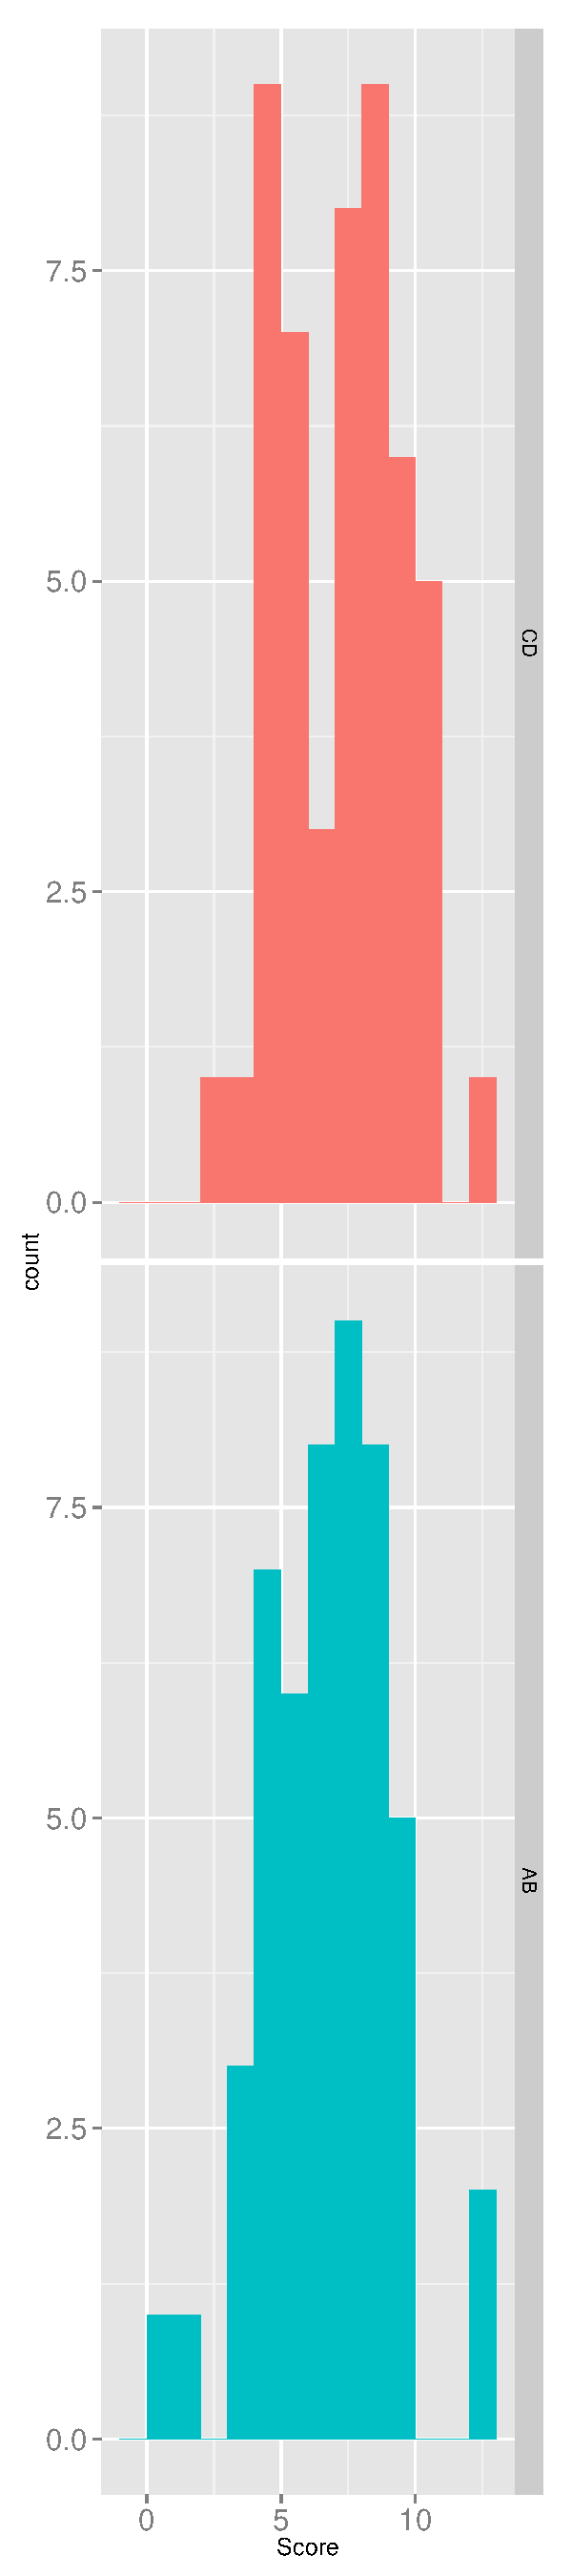
\includegraphics[width=0.95\linewidth]{Topic06_overallscore}
\caption{\label{mar:hist}Histograms of overall scores by section. The support of the scores is [0,25].}\end{marginfigure}% latex table generated in R 3.2.2 by xtable 1.8-0 package
% Mon Nov 23 01:15:44 2015
\begin{longtable}{rrrrrrrrrr}
  \hline
 & Mean & Std.dev &   &   & Min & Q1 & Median & Q3 & Max \\ 
  \hline
CD & 6.76 & 2.27 &  &  & 2.00 & 5.00 & 7.00 & 8.00 & 12.00 \\ 
  AB & 6.24 & 2.38 &  &  & 0.00 & 5.00 & 6.00 & 8.00 & 12.00 \\ 
   \hline
\hline
\caption{Summary of overall scores by section. Sections are ordered from the highest mean score to the lowest.} 
\label{tab:summary}
\end{longtable}
\begin{center}
\begin{wrapfigure}{o}{0.8\columnwidth}
\begin{centering}
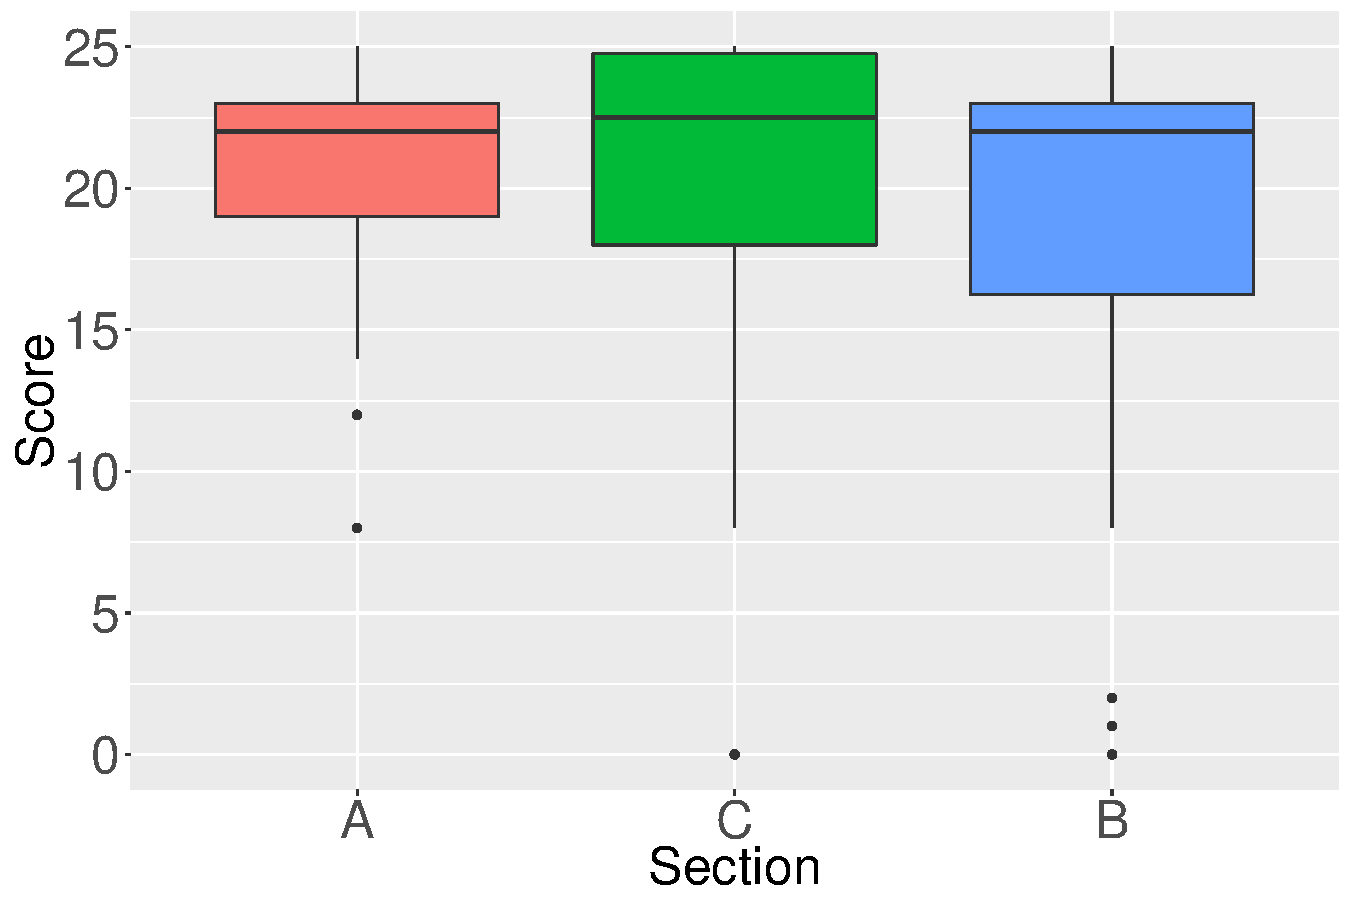
\includegraphics[width=0.8\linewidth]{Topic06_boxplot_score}
\par\end{centering}
\caption{\label{fig:boxplot-score}Boxplot for the overall scores by section. The highest median comes from Section AB,CD.}
\end{wrapfigure}\par\end{center}


\clearpage
\newpage{}
\section{Learning Outcomes}

\bigskip{}

The learning outcomes in this topic are:

\bigskip{}
Use standardizing to determine how many standard deviations an observation is away from the mean value.

 \bigskip{} 

Use z-scores to compare observations for different quantitative variables.

 \bigskip{} 

Explain how standardizing affects the shape, center, and variability of the distribution of a quantitative variable.

 \bigskip{} 

Determine which quantitative variables could be modeled using the normal distribution by interpreting graphical representations of the variable.

 \bigskip{} 

Apply the 68-95-99.

 \bigskip{} 

Find percentile or area values for any given observation from a normal distribution.

 \bigskip{} 

Find the value of an observation when given a percentile or area value from the normal distribution.
\\ 
 ~~ 


\clearpage
\newpage{}

Figure \ref{mar:LOpct} displays the percentage correct of each question by section. The graph is facetted by learning outcome. In addition, sections are ordered by their overall mean scores and learning outcomes are ordered by their average percentage correct scores.

Table \ref{tab:Oset} and Figure \ref{sbsb-os} give the average percentages correct for each learning outcome. The learning outcome D has the highest correct percentage, and  E has the lowest average correct percent.

\begin{marginfigure}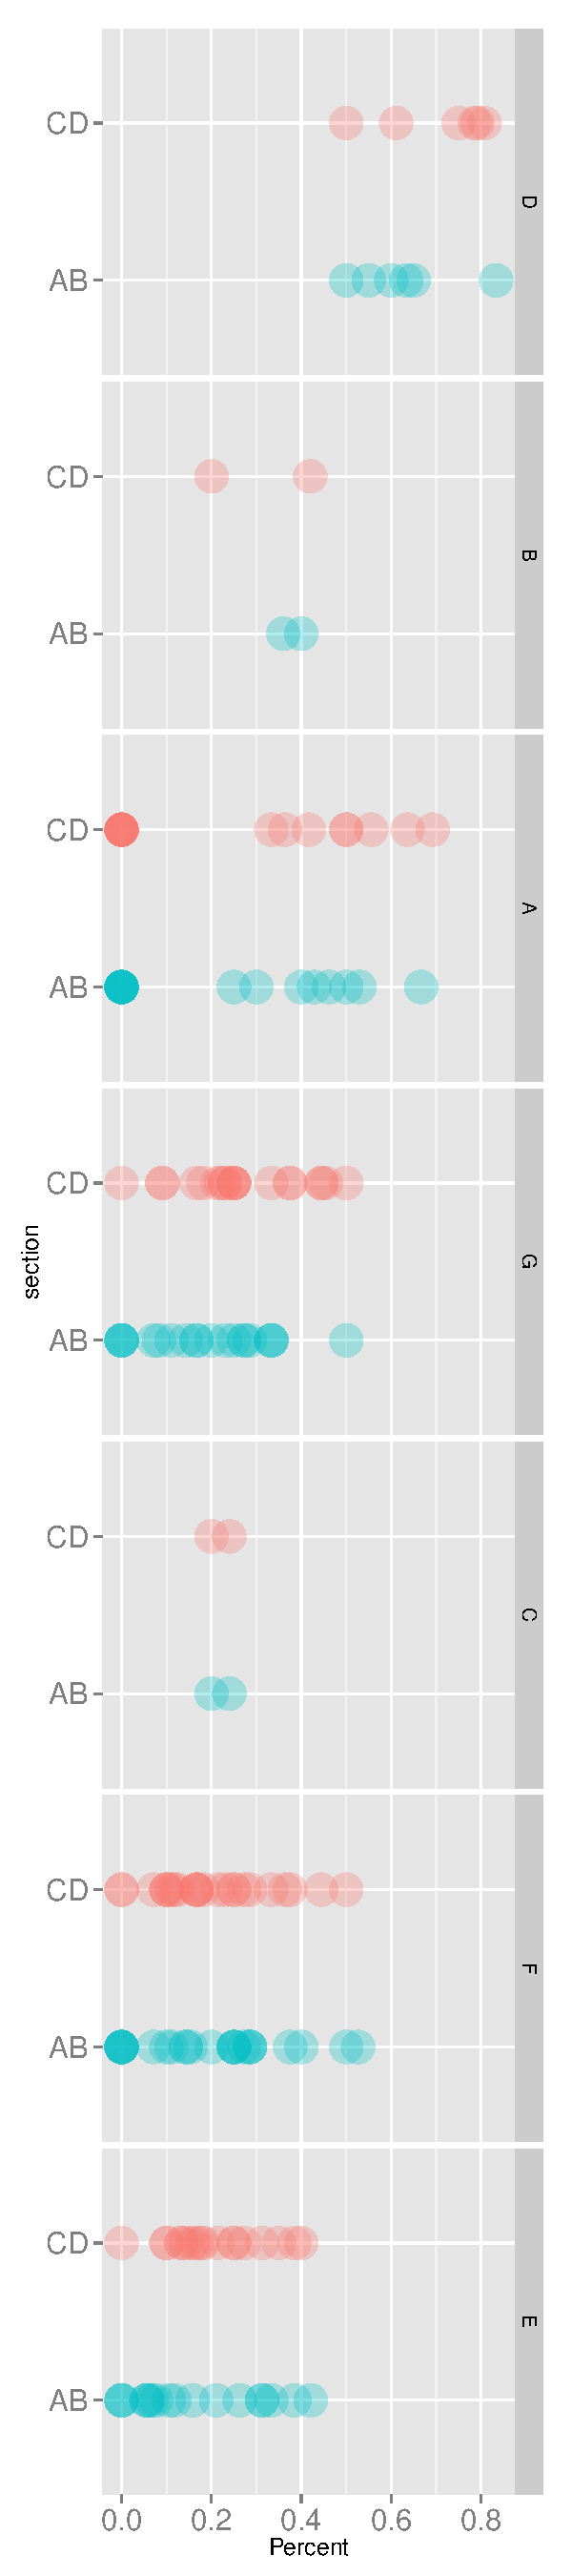
\includegraphics[width=0.95\linewidth]{Topic06_Scatterplot_LOpct}
\caption{\label{mar:LOpct}Scatterplot of correct percentage by learning outcome. The sections are sorted by their overall mean scores, and the learning outcomes are ordered by the mean correct percentage.}\end{marginfigure}% latex table generated in R 3.2.2 by xtable 1.8-0 package
% Mon Nov 23 01:15:44 2015
\begin{longtable}{rrr}
  \hline
 & CD & AB \\ 
  \hline
D & 72.00 & 61.00 \\ 
  B & 31.00 & 38.00 \\ 
  A & 25.50 & 23.00 \\ 
  G & 26.00 & 21.50 \\ 
  C & 22.00 & 22.00 \\ 
  F & 19.20 & 20.80 \\ 
  E & 20.67 & 16.67 \\ 
   \hline
\hline
\caption{Average percentages correct for each learning outcome by section. The learning outcomes are sorted by the average percentages correct of all sections, from the highest to the lowest.} 
\label{tab:Oset}
\end{longtable}
\begin{center}
\begin{wrapfigure}{o}{0.98\columnwidth}
\begin{centering}
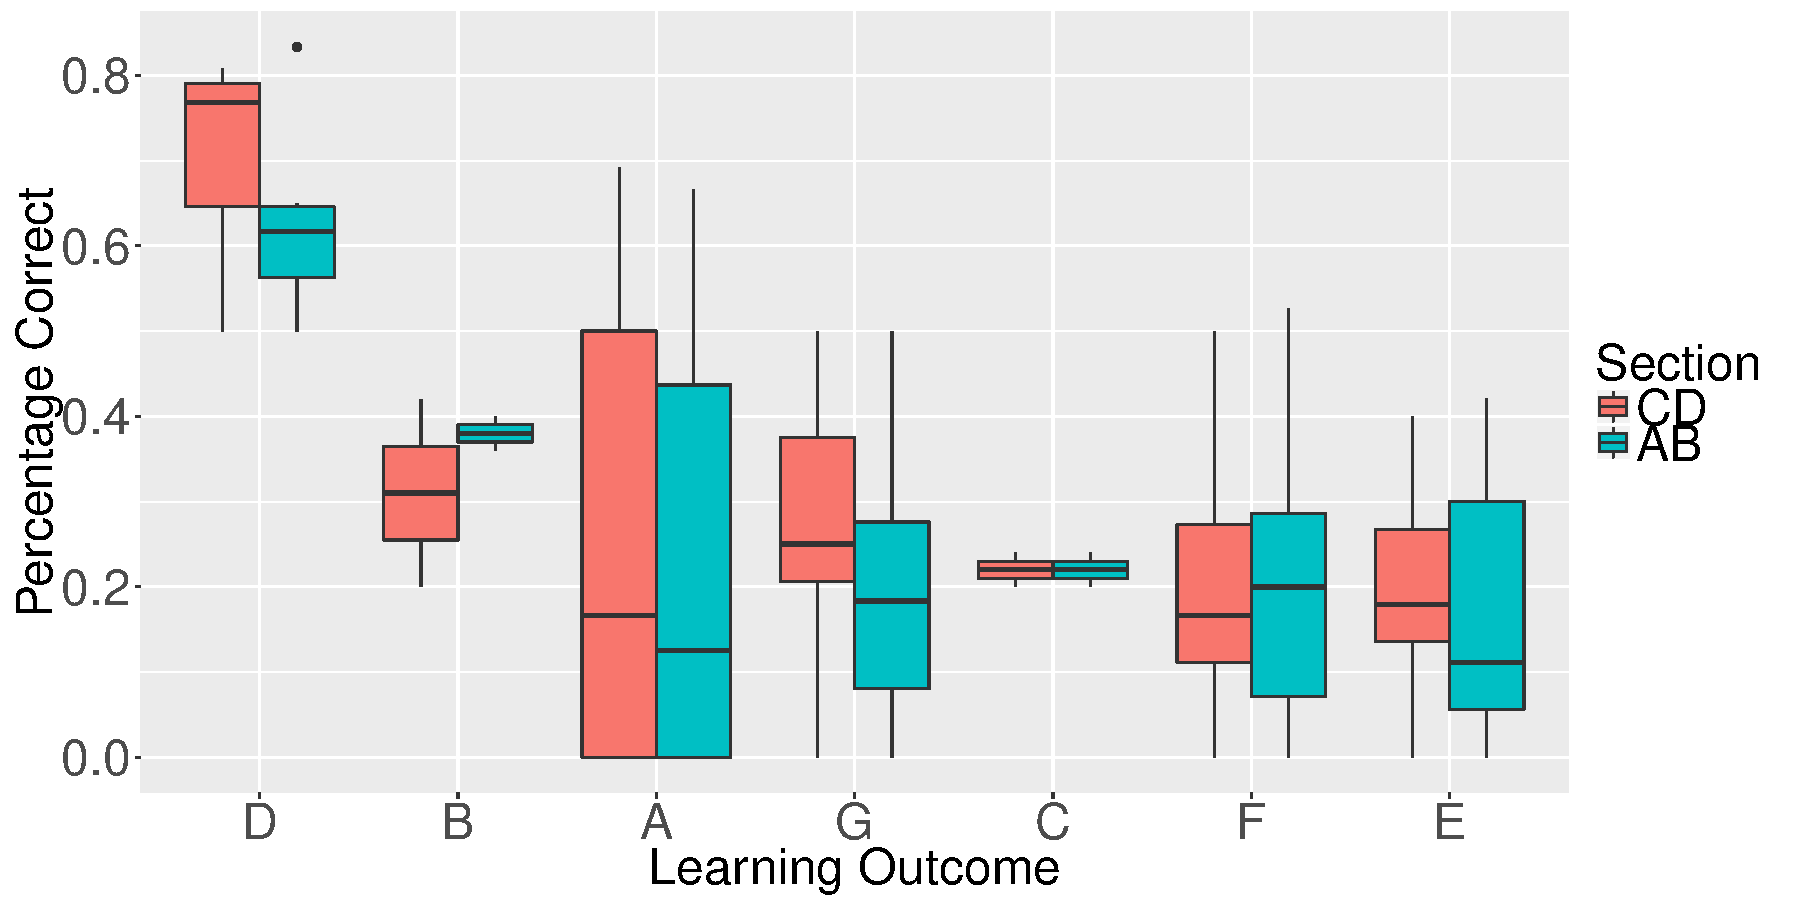
\includegraphics[width=0.98\linewidth]{Topic06_Sidebyside_Boxplots_LearningObj}
\par\end{centering}
\caption{\label{sbsb-os}Side-by-side boxplots for learning outcomes by section. The learning outcome on the left has the highest average correct percentage, while the one on the right has the lowest.}
\end{wrapfigure}
\par\end{center}

\clearpage
\newpage{}

To analyze the students' performance by section and learning outcomes, 
we consider the generalized linear mixed model:
\[
g(E[Y_{ijk}|u_{jk}])= \mu+\tau_{i}+s_{j}+\tau s_{ij}+u_{jk}
\]
where $i=1,...,$7 learning outcomes; 
$j=1,...,$2 sections; $k=1,...,n_j$ students.
$Y_{ijk}$ is the score (scaled in $[0,1]$) of the $k$th student of 
section $j$ in the $i$th learning outcome. $\tau_i$ and $s_{j}$ are the 
fixed effects of learning outcome $i$ and section $j$. 
$\tau s_{ij}$ is the interaction between the two factors.
$u_{jk}$ is the random effect from the students with 
$u_{jk} \sim N(0,\sigma_{u}^{2})$.

By default the software R sets $\tau_{1}=0$, $s_{1}=0$ and 
$\tau s_{ij}=0, \forall i,j = 1 $ as the identifiability constraints.

Table \ref{tab:pvalues_obj} and \ref{tab:pvalues_sec} present the p-values 
of multiple comparison in the learning outcomes and the sections. 
The result of the model is as follows.

% latex table generated in R 3.2.2 by xtable 1.8-0 package
% Mon Nov 23 01:15:45 2015
\begin{longtable}{rrrrrrr}
  \hline
 & D & B & G & A & C & E \\ 
  \hline
B & 0.0000 &  &  &  &  &  \\ 
  G & 0.0000 & 1.0000 &  &  &  &  \\ 
  A & 0.0000 & 1.0000 & 1.0000 &  &  &  \\ 
  C & 0.0000 & 1.0000 & 1.0000 & 1.0000 &  &  \\ 
  E & 0.0000 & 1.0000 & 1.0000 & 1.0000 & 1.0000 &  \\ 
  F & 0.0000 & 0.3627 & 1.0000 & 1.0000 & 1.0000 & 1.0000 \\ 
   \hline
\hline
\caption{P-values of the multiple comparison between learning outcomes} 
\label{tab:pvalues_obj}
\end{longtable}
% latex table generated in R 3.2.2 by xtable 1.8-0 package
% Mon Nov 23 01:15:46 2015
\begin{longtable}{rr}
  \hline
 & CD \\ 
  \hline
AB & 0.0336 \\ 
   \hline
\hline
\caption{P-values of the multiple comparison between sections} 
\label{tab:pvalues_sec}
\end{longtable}


\begin{knitrout}
\definecolor{shadecolor}{rgb}{0.969, 0.969, 0.969}\color{fgcolor}\begin{kframe}
\begin{verbatim}
## Generalized linear mixed model fit by maximum likelihood (Adaptive
##   Gauss-Hermite Quadrature, nAGQ = 0) [glmerMod]
##  Family: binomial  ( logit )
## Formula: 
## Score ~ Objective * Section + (1 | student) + (1 | Section:student)
##    Data: Learning_Objectives
## Weights: FullPoints
## 
##      AIC      BIC   logLik deviance df.resid 
##   1783.7   1856.5   -875.8   1751.7      684 
## 
## Scaled residuals: 
##     Min      1Q  Median      3Q     Max 
## -2.9874 -0.8716  0.0052  0.8666  4.1551 
## 
## Random effects:
##  Groups          Name        Variance Std.Dev.
##  student         (Intercept) 0.1190   0.3450  
##  Section:student (Intercept) 0.1213   0.3483  
## Number of obs: 700, groups:  student, 100; Section:student, 100
## 
## Fixed effects:
##                      Estimate Std. Error z value Pr(>|z|)    
## (Intercept)            0.9672     0.1737   5.568 2.58e-08 ***
## ObjectiveB            -1.7870     0.2707  -6.602 4.06e-11 ***
## ObjectiveA            -2.0647     0.2814  -7.336 2.20e-13 ***
## ObjectiveG            -2.0380     0.2802  -7.272 3.54e-13 ***
## ObjectiveC            -2.2619     0.2129 -10.623  < 2e-16 ***
## ObjectiveF            -2.4362     0.2276 -10.705  < 2e-16 ***
## ObjectiveE            -2.3427     0.2379  -9.848  < 2e-16 ***
## SectionAB             -0.5068     0.2381  -2.129   0.0333 *  
## ObjectiveB:SectionAB   0.8203     0.3725   2.203   0.0276 *  
## ObjectiveA:SectionAB   0.3607     0.3984   0.905   0.3653    
## ObjectiveG:SectionAB   0.2454     0.4011   0.612   0.5406    
## ObjectiveC:SectionAB   0.4993     0.2950   1.693   0.0905 .  
## ObjectiveF:SectionAB   0.6008     0.3137   1.915   0.0555 .  
## ObjectiveE:SectionAB   0.2299     0.3393   0.678   0.4980    
## ---
## Signif. codes:  0 '***' 0.001 '**' 0.01 '*' 0.05 '.' 0.1 ' ' 1
## 
## Correlation of Fixed Effects:
##             (Intr) ObjctB ObjctA ObjctG ObjctC ObjctF ObjctE SctnAB OB:SAB
## ObjectiveB  -0.540                                                        
## ObjectiveA  -0.520  0.335                                                 
## ObjectiveG  -0.522  0.336  0.324                                          
## ObjectiveC  -0.687  0.443  0.426  0.428                                   
## ObjectiveF  -0.643  0.414  0.399  0.401  0.528                            
## ObjectiveE  -0.615  0.396  0.382  0.383  0.505  0.472                     
## SectionAB   -0.730  0.394  0.379  0.381  0.502  0.469  0.449              
## ObjctvB:SAB  0.393 -0.727 -0.243 -0.244 -0.322 -0.301 -0.288 -0.531       
## ObjctvA:SAB  0.367 -0.236 -0.706 -0.229 -0.301 -0.282 -0.270 -0.497  0.319
## ObjctvG:SAB  0.365 -0.235 -0.226 -0.699 -0.299 -0.280 -0.268 -0.494  0.317
## ObjctvC:SAB  0.496 -0.320 -0.308 -0.309 -0.722 -0.381 -0.364 -0.671  0.431
## ObjctvF:SAB  0.467 -0.301 -0.289 -0.291 -0.383 -0.725 -0.343 -0.631  0.405
## ObjctvE:SAB  0.431 -0.278 -0.268 -0.269 -0.354 -0.331 -0.701 -0.584  0.375
##             OA:SAB OG:SAB OC:SAB OF:SAB
## ObjectiveB                             
## ObjectiveA                             
## ObjectiveG                             
## ObjectiveC                             
## ObjectiveF                             
## ObjectiveE                             
## SectionAB                              
## ObjctvB:SAB                            
## ObjctvA:SAB                            
## ObjctvG:SAB  0.296                     
## ObjctvC:SAB  0.403  0.401              
## ObjctvF:SAB  0.379  0.377  0.513       
## ObjctvE:SAB  0.351  0.349  0.474  0.446
\end{verbatim}
\end{kframe}
\end{knitrout}


\clearpage
\newpage{}

\section{Question Sets}
The question set is a set of questions which are randomly delivered to the students. The questions in each question set cover the same learning outcome and should be equally difficult. 

The average percentages correct for question sets are shown in Table \ref{tab:Qset-mean} and Figure \ref{mar:Qsetpct}. Among all the 21 question sets, question set I has the highest correct percentage. C is the hardest question set which has the lowest average score.

\begin{marginfigure}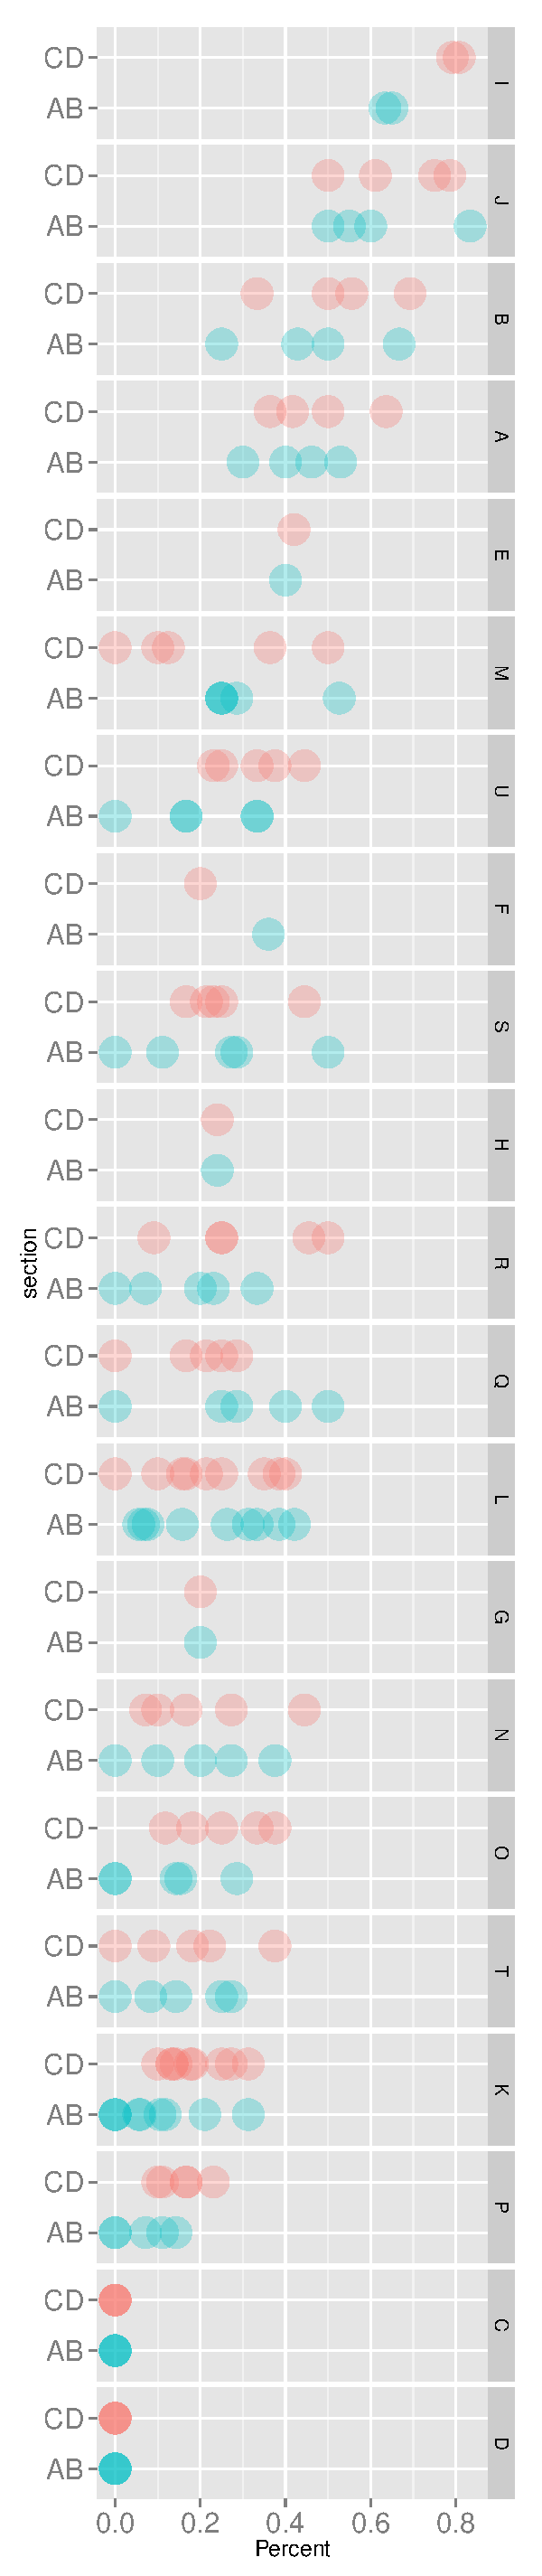
\includegraphics[width=0.95\linewidth]{Topic06_Scatterplot_QSetpct}
\caption{\label{mar:Qsetpct}Scatterplot of Correct Percentage by Question Set.}\end{marginfigure}% latex table generated in R 3.2.2 by xtable 1.8-0 package
% Mon Nov 23 01:15:47 2015
\begin{longtable}{cc|cc|cc}
  \hline
Qset & LO & \#Qn & Overall & CD & AB \\ 
  \hline
I & D &   2 & 72.00 & 80.00 & 64.00 \\ 
  J & D &   4 & 61.00 & 64.00 & 58.00 \\ 
  B & A &   4 & 51.00 & 54.00 & 48.00 \\ 
  A & A &   4 & 46.00 & 48.00 & 44.00 \\ 
  E & B &   1 & 41.00 & 42.00 & 40.00 \\ 
  M & F &   5 & 29.00 & 22.00 & 36.00 \\ 
  U & G &   5 & 29.00 & 32.00 & 26.00 \\ 
  F & B &   1 & 28.00 & 20.00 & 36.00 \\ 
  S & G &   5 & 26.00 & 26.00 & 26.00 \\ 
  H & C &   1 & 24.00 & 24.00 & 24.00 \\ 
  R & G &   5 & 24.00 & 30.00 & 18.00 \\ 
  Q & F &   5 & 23.00 & 16.00 & 30.00 \\ 
  L & E &   9 & 22.67 & 22.00 & 23.33 \\ 
  G & C &   1 & 20.00 & 20.00 & 20.00 \\ 
  N & F &   5 & 19.00 & 20.00 & 18.00 \\ 
  O & F &   5 & 18.00 & 22.00 & 14.00 \\ 
  T & G &   5 & 16.00 & 16.00 & 16.00 \\ 
  K & E &   9 & 14.67 & 19.33 & 10.00 \\ 
  P & F &   5 & 11.00 & 16.00 & 6.00 \\ 
  C & A &   4 & 0.00 & 0.00 & 0.00 \\ 
  D & A &   4 & 0.00 & 0.00 & 0.00 \\ 
   \hline
\hline
\caption{Average percentages correct for each question set by section. The question sets are sorted by the section means. The second column indicates the corresponding learning outcomes.} 
\label{tab:Qset-mean}
\end{longtable}


Table \ref{tab:Qset-sd} presents the standard deviation of the question correct rates by question set and section.
%%%% ONLY COMMENTED OUT FOR TESTING!!!!!!!!!!!!!!!!!!! %%%%%%%%%%%%
%Question set rownames(d[d[,3]>1,4:9])[which.min(rowMeans(d[d[,3]>1,4:9]))] has the smallest standard deviation, while rownames(d[,4:9])[which.max(rowMeans(d[,4:9]))] has the largest standard deviation.

% latex table generated in R 3.2.2 by xtable 1.8-0 package
% Mon Nov 23 01:15:47 2015
\begin{longtable}{cc|cc|cc}
  \hline
Qset & LO & \#Qn & Overall & CD & AB \\ 
  \hline
I & D &   2 & 9.17 & 1.13 & 1.18 \\ 
  J & D &   4 & 13.12 & 13.15 & 14.74 \\ 
  B & A &   4 & 15.24 & 14.85 & 17.26 \\ 
  A & A &   4 & 10.50 & 11.89 & 9.74 \\ 
  E & B &   1 & 1.41 & 0.00 & 0.00 \\ 
  M & F &   5 & 16.71 & 20.67 & 12.06 \\ 
  U & G &   5 & 12.88 & 8.85 & 13.94 \\ 
  F & B &   1 & 11.31 & 0.00 & 0.00 \\ 
  S & G &   5 & 14.62 & 10.70 & 19.03 \\ 
  H & C &   1 & 0.00 & 0.00 & 0.00 \\ 
  R & G &   5 & 16.07 & 16.75 & 13.21 \\ 
  Q & F &   5 & 15.58 & 11.15 & 18.83 \\ 
  L & E &   9 & 13.54 & 13.54 & 14.35 \\ 
  G & C &   1 & 0.00 & 0.00 & 0.00 \\ 
  N & F &   5 & 14.09 & 15.17 & 14.61 \\ 
  O & F &   5 & 12.83 & 10.57 & 12.03 \\ 
  T & G &   5 & 12.18 & 14.14 & 11.41 \\ 
  K & E &   9 & 10.09 & 7.28 & 10.68 \\ 
  P & F &   5 & 7.29 & 5.24 & 6.46 \\ 
  C & A &   4 & 0.00 & 0.00 & 0.00 \\ 
  D & A &   4 & 0.00 & 0.00 & 0.00 \\ 
   \hline
\hline
\caption{Standard deviations of the percentages correct by section. The second column indicates the corresponding learning outcomes. The third column gives the number of questions in each question set.} 
\label{tab:Qset-sd}
\end{longtable}



\clearpage
\newpage{}
\subsection{Questions}

Table \ref{tab:summary_question} compares the performance on each question. 

% latex table generated in R 3.2.2 by xtable 1.8-0 package
% Mon Nov 23 01:15:47 2015
\begin{longtable}{cccl|cccc|ccccc|l}
  \hline
ID & LO & Qset & Name & Type & FullPt & QinSet & N & CrtPct & Count & NA's & Mean & Std & Flag \\ 
  \hline
\hyperlink{T06.A.A.04.1.1.MC.1.2}{1} & A & A & 1 & MC &   1 &   1 &   4 & 46.15 &  26 &  74 & 0.46 & 0.51 &  \\ 
  \hyperlink{T06.A.A.04.1.1.MC.2.2}{2} & A & A & 2 & MC &   1 &   1 &   4 & 54.17 &  24 &  76 & 0.54 & 0.51 & * \\ 
  \hyperlink{T06.A.A.04.1.1.MC.3.2}{3} & A & A & 3 & MC &   1 &   1 &   4 & 36.36 &  22 &  78 & 0.36 & 0.49 & * \\ 
  \hyperlink{T06.A.A.04.1.1.MC.4.2}{4} & A & A & 4 & MC &   1 &   1 &   4 & 46.43 &  28 &  72 & 0.46 & 0.51 &  \\ 
   &  &  &  &  &  &  &  &  &  &  &  &  &  \\ 
  \hyperlink{T06.A.B.04.1.1.MC.1.2}{5} & A & B & 1 & MC &   1 &   1 &   4 & 50.00 &  32 &  68 & 0.50 & 0.51 &  \\ 
  \hyperlink{T06.A.B.04.1.1.MC.2.2}{6} & A & B & 2 & MC &   1 &   1 &   4 & 50.00 &  26 &  74 & 0.50 & 0.51 &  \\ 
  \hyperlink{T06.A.B.04.1.1.MC.3.2}{7} & A & B & 3 & MC &   1 &   1 &   4 & 52.38 &  21 &  79 & 0.52 & 0.51 &  \\ 
  \hyperlink{T06.A.B.04.1.1.MC.4.2}{8} & A & B & 4 & MC &   1 &   1 &   4 & 52.38 &  21 &  79 & 0.52 & 0.51 &  \\ 
   &  &  &  &  &  &  &  &  &  &  &  &  &  \\ 
  \hyperlink{T06.A.C.04.1.1.FB.1.2}{9} & A & C & 1 & FB &   1 &   1 &   4 & 0.00 &  23 &  77 & 0.00 & 0.00 &  \\ 
  \hyperlink{T06.A.C.04.1.1.FB.2.2}{10} & A & C & 2 & FB &   1 &   1 &   4 & 0.00 &  27 &  73 & 0.00 & 0.00 &  \\ 
  \hyperlink{T06.A.C.04.1.1.FB.3.2}{11} & A & C & 3 & FB &   1 &   1 &   4 & 0.00 &  23 &  77 & 0.00 & 0.00 &  \\ 
  \hyperlink{T06.A.C.04.1.1.FB.4.2}{12} & A & C & 4 & FB &   1 &   1 &   4 & 0.00 &  27 &  73 & 0.00 & 0.00 &  \\ 
   &  &  &  &  &  &  &  &  &  &  &  &  &  \\ 
  \hyperlink{T06.A.D.04.1.1.FB.1.2}{13} & A & D & 1 & FB &   1 &   1 &   4 & 0.00 &  20 &  80 & 0.00 & 0.00 &  \\ 
  \hyperlink{T06.A.D.04.1.1.FB.2.2}{14} & A & D & 2 & FB &   1 &   1 &   4 & 0.00 &  27 &  73 & 0.00 & 0.00 &  \\ 
  \hyperlink{T06.A.D.04.1.1.FB.3.2}{15} & A & D & 3 & FB &   1 &   1 &   4 & 0.00 &  24 &  76 & 0.00 & 0.00 &  \\ 
  \hyperlink{T06.A.D.04.1.1.FB.4.2}{16} & A & D & 4 & FB &   1 &   1 &   4 & 0.00 &  29 &  71 & 0.00 & 0.00 &  \\ 
   &  &  &  &  &  &  &  &  &  &  &  &  &  \\ 
  \hyperlink{T06.B.E.01.1.1.MC.compare1.2}{17} & B & E & compare1 & MC &   1 &   1 &   1 & 41.00 & 100 &   0 & 0.41 & 0.49 &  \\ 
   &  &  &  &  &  &  &  &  &  &  &  &  &  \\ 
  \hyperlink{T06.B.F.01.1.1.MC.compare2.2}{18} & B & F & compare2 & MC &   1 &   1 &   1 & 28.00 & 100 &   0 & 0.28 & 0.45 &  \\ 
   &  &  &  &  &  &  &  &  &  &  &  &  &  \\ 
  \hyperlink{T06.C.G.01.1.1.MC.1.2}{19} & C & G & 1 & MC &   1 &   1 &   1 & 20.00 & 100 &   0 & 0.20 & 0.40 &  \\ 
   &  &  &  &  &  &  &  &  &  &  &  &  &  \\ 
  \hyperlink{T06.C.H.01.1.1.MC.1.2}{20} & C & H & 1 & MC &   1 &   1 &   1 & 24.00 & 100 &   0 & 0.24 & 0.43 &  \\ 
   &  &  &  &  &  &  &  &  &  &  &  &  &  \\ 
  \hyperlink{T06.D.I.02.1.1.TF.feet.2}{21} & D & I & feet & TF &   1 &   1 &   2 & 73.91 &  46 &  54 & 0.74 & 0.44 &  \\ 
  \hyperlink{T06.D.I.02.1.1.TF.lowtemp.2}{22} & D & I & lowtemp & TF &   1 &   1 &   2 & 70.37 &  54 &  46 & 0.70 & 0.46 &  \\ 
   &  &  &  &  &  &  &  &  &  &  &  &  &  \\ 
  \hyperlink{T06.D.J.04.1.1.TF.gain.2}{23} & D & J & gain & TF &   1 &   1 &   4 & 60.71 &  28 &  72 & 0.61 & 0.50 & * \\ 
  \hyperlink{T06.D.J.04.1.1.TF.mpg.2}{24} & D & J & mpg & TF &   1 &   1 &   4 & 80.00 &  10 &  90 & 0.80 & 0.42 & * \\ 
  \hyperlink{T06.D.J.04.1.1.TF.blowhole.2}{25} & D & J & blowhole & TF &   1 &   1 &   4 & 64.29 &  28 &  72 & 0.64 & 0.49 & * \\ 
  \hyperlink{T06.D.J.04.1.1.TF.CDs.2}{26} & D & J & CDs & TF &   1 &   1 &   4 & 52.94 &  34 &  66 & 0.53 & 0.51 & * \\ 
   &  &  &  &  &  &  &  &  &  &  &  &  &  \\ 
  \hyperlink{T06.E.K.09.3.1.FB.whale1.2}{27} & E & K & whale1 & FB &   1 &   3 &   9 & 25.71 &  35 &  65 & 0.26 & 0.44 & * \\ 
  \hyperlink{T06.E.K.09.3.1.FB.whale2.2}{28} & E & K & whale2 & FB &   1 &   3 &   9 & 6.06 &  33 &  67 & 0.06 & 0.24 & * \\ 
  \hyperlink{T06.E.K.09.3.1.FB.whale3.2}{29} & E & K & whale3 & FB &   1 &   3 &   9 & 14.71 &  34 &  66 & 0.15 & 0.36 &  \\ 
  \hyperlink{T06.E.K.09.3.1.FB.cow1.2}{30} & E & K & cow1 & FB &   1 &   3 &   9 & 17.65 &  34 &  66 & 0.18 & 0.39 &  \\ 
  \hyperlink{T06.E.K.09.3.1.FB.cow2.2}{31} & E & K & cow2 & FB &   1 &   3 &   9 & 7.89 &  38 &  62 & 0.08 & 0.27 & * \\ 
  \hyperlink{T06.E.K.09.3.1.FB.cow3.2}{32} & E & K & cow3 & FB &   1 &   3 &   9 & 14.29 &  28 &  72 & 0.14 & 0.36 &  \\ 
  \hyperlink{T06.E.K.09.3.1.FB.bulbs1.2}{33} & E & K & bulbs1 & FB &   1 &   3 &   9 & 22.58 &  31 &  69 & 0.23 & 0.43 & * \\ 
  \hyperlink{T06.E.K.09.3.1.FB.bulbs2.2}{34} & E & K & bulbs2 & FB &   1 &   3 &   9 & 9.68 &  31 &  69 & 0.10 & 0.30 & * \\ 
  \hyperlink{T06.E.K.09.3.1.FB.bulbs3.2}{35} & E & K & bulbs3 & FB &   1 &   3 &   9 & 13.89 &  36 &  64 & 0.14 & 0.35 &  \\ 
   &  &  &  &  &  &  &  &  &  &  &  &  &  \\ 
  \hyperlink{T06.E.L.09.3.1.MC.heights1.2}{36} & E & L & heights1 & MC &   1 &   3 &   9 & 15.79 &  38 &  62 & 0.16 & 0.37 & * \\ 
  \hyperlink{T06.E.L.09.3.1.MC.heights2.2}{37} & E & L & heights2 & MC &   1 &   3 &   9 & 15.79 &  38 &  62 & 0.16 & 0.37 & * \\ 
  \hyperlink{T06.E.L.09.3.1.MC.heights3.2}{38} & E & L & heights3 & MC &   1 &   3 &   9 & 38.46 &  39 &  61 & 0.38 & 0.49 & * \\ 
  \hyperlink{T06.E.L.09.3.1.MC.mm1.2}{39} & E & L & mm1 & MC &   1 &   3 &   9 & 3.33 &  30 &  70 & 0.03 & 0.18 & * \\ 
  \hyperlink{T06.E.L.09.3.1.MC.mm2.2}{40} & E & L & mm2 & MC &   1 &   3 &   9 & 26.67 &  30 &  70 & 0.27 & 0.45 & * \\ 
  \hyperlink{T06.E.L.09.3.1.MC.mm3.2}{41} & E & L & mm3 & MC &   1 &   3 &   9 & 17.95 &  39 &  61 & 0.18 & 0.39 & * \\ 
  \hyperlink{T06.E.L.09.3.1.MC.IQ1.2}{42} & E & L & IQ1 & MC &   1 &   3 &   9 & 36.36 &  33 &  67 & 0.36 & 0.49 & * \\ 
  \hyperlink{T06.E.L.09.3.1.MC.IQ2.2}{43} & E & L & IQ2 & MC &   1 &   3 &   9 & 28.00 &  25 &  75 & 0.28 & 0.46 & * \\ 
  \hyperlink{T06.E.L.09.3.1.MC.IQ3.2}{44} & E & L & IQ3 & MC &   1 &   3 &   9 & 21.43 &  28 &  72 & 0.21 & 0.42 & * \\ 
   &  &  &  &  &  &  &  &  &  &  &  &  &  \\ 
  \hyperlink{T06.F.M.05.1.1.MC.mm1.2}{45} & F & M & mm1 & MC &   1 &   1 &   5 & 40.74 &  27 &  73 & 0.41 & 0.50 & * \\ 
  \hyperlink{T06.F.M.05.1.1.MC.Bulb1.2}{46} & F & M & Bulb1 & MC &   1 &   1 &   5 & 16.67 &  18 &  82 & 0.17 & 0.38 & * \\ 
  \hyperlink{T06.F.M.05.1.1.MC.IQ1.2}{47} & F & M & IQ1 & MC &   1 &   1 &   5 & 31.58 &  19 &  81 & 0.32 & 0.48 & * \\ 
  \hyperlink{T06.F.M.05.1.1.MC.Whale1.2}{48} & F & M & Whale1 & MC &   1 &   1 &   5 & 41.18 &  17 &  83 & 0.41 & 0.51 & * \\ 
  \hyperlink{T06.F.M.05.1.1.MC.Cow1.2}{49} & F & M & Cow1 & MC &   1 &   1 &   5 & 10.53 &  19 &  81 & 0.11 & 0.32 & * \\ 
   &  &  &  &  &  &  &  &  &  &  &  &  &  \\ 
  \hyperlink{T06.F.N.05.1.1.MC.mm2.2}{50} & F & N & mm2 & MC &   1 &   1 &   5 & 22.22 &  18 &  82 & 0.22 & 0.43 & * \\ 
  \hyperlink{T06.F.N.05.1.1.MC.Bulb2.2}{51} & F & N & Bulb2 & MC &   1 &   1 &   5 & 5.88 &  17 &  83 & 0.06 & 0.24 & * \\ 
  \hyperlink{T06.F.N.05.1.1.MC.IQ2.2}{52} & F & N & IQ2 & MC &   1 &   1 &   5 & 27.27 &  22 &  78 & 0.27 & 0.46 & * \\ 
  \hyperlink{T06.F.N.05.1.1.MC.Whale2.2}{53} & F & N & Whale2 & MC &   1 &   1 &   5 & 26.32 &  19 &  81 & 0.26 & 0.45 & * \\ 
  \hyperlink{T06.F.N.05.1.1.MC.Cow2.2}{54} & F & N & Cow2 & MC &   1 &   1 &   5 & 12.50 &  24 &  76 & 0.12 & 0.34 &  \\ 
   &  &  &  &  &  &  &  &  &  &  &  &  &  \\ 
  \hyperlink{T06.F.O.05.1.1.MC.mm3.2}{55} & F & O & mm3 & MC &   1 &   1 &   5 & 20.00 &  15 &  85 & 0.20 & 0.41 &  \\ 
  \hyperlink{T06.F.O.05.1.1.MC.Bulb3.2}{56} & F & O & Bulb3 & MC &   1 &   1 &   5 & 14.29 &  14 &  86 & 0.14 & 0.36 &  \\ 
  \hyperlink{T06.F.O.05.1.1.MC.IQ3.2}{57} & F & O & IQ3 & MC &   1 &   1 &   5 & 8.00 &  25 &  75 & 0.08 & 0.28 & * \\ 
  \hyperlink{T06.F.O.05.1.1.MC.Whale3.2}{58} & F & O & Whale3 & MC &   1 &   1 &   5 & 24.00 &  25 &  75 & 0.24 & 0.44 & * \\ 
  \hyperlink{T06.F.O.05.1.1.MC.Cow3.2}{59} & F & O & Cow3 & MC &   1 &   1 &   5 & 23.81 &  21 &  79 & 0.24 & 0.44 & * \\ 
   &  &  &  &  &  &  &  &  &  &  &  &  &  \\ 
  \hyperlink{T06.F.P.05.1.1.MC.mm4.2}{60} & F & P & mm4 & MC &   1 &   1 &   5 & 8.70 &  23 &  77 & 0.09 & 0.29 &  \\ 
  \hyperlink{T06.F.P.05.1.1.MC.Bulb4.2}{61} & F & P & Bulb4 & MC &   1 &   1 &   5 & 5.88 &  17 &  83 & 0.06 & 0.24 &  \\ 
  \hyperlink{T06.F.P.05.1.1.MC.IQ4.2}{62} & F & P & IQ4 & MC &   1 &   1 &   5 & 20.00 &  20 &  80 & 0.20 & 0.41 &  \\ 
  \hyperlink{T06.F.P.05.1.1.MC.Whale4.2}{63} & F & P & Whale4 & MC &   1 &   1 &   5 & 5.26 &  19 &  81 & 0.05 & 0.23 &  \\ 
  \hyperlink{T06.F.P.05.1.1.MC.Cow4.2}{64} & F & P & Cow4 & MC &   1 &   1 &   5 & 14.29 &  21 &  79 & 0.14 & 0.36 &  \\ 
   &  &  &  &  &  &  &  &  &  &  &  &  &  \\ 
  \hyperlink{T06.F.Q.05.1.1.MC.mm5.2}{65} & F & Q & mm5 & MC &   1 &   1 &   5 & 27.78 &  18 &  82 & 0.28 & 0.46 & * \\ 
  \hyperlink{T06.F.Q.05.1.1.MC.Bulb5.2}{66} & F & Q & Bulb5 & MC &   1 &   1 &   5 & 26.32 &  19 &  81 & 0.26 & 0.45 & * \\ 
  \hyperlink{T06.F.Q.05.1.1.MC.IQ5.2}{67} & F & Q & IQ5 & MC &   1 &   1 &   5 & 10.53 &  19 &  81 & 0.11 & 0.32 & * \\ 
  \hyperlink{T06.F.Q.05.1.1.MC.Whale5.2}{68} & F & Q & Whale5 & MC &   1 &   1 &   5 & 27.27 &  11 &  89 & 0.27 & 0.47 & * \\ 
  \hyperlink{T06.F.Q.05.1.1.MC.Cow5.2}{69} & F & Q & Cow5 & MC &   1 &   1 &   5 & 24.24 &  33 &  67 & 0.24 & 0.44 &  \\ 
   &  &  &  &  &  &  &  &  &  &  &  &  &  \\ 
  \hyperlink{T06.G.R.05.1.1.MC.mm1.2}{70} & G & R & mm1 & MC &   1 &   1 &   5 & 33.33 &  21 &  79 & 0.33 & 0.48 & * \\ 
  \hyperlink{T06.G.R.05.1.1.MC.Bulb1.2}{71} & G & R & Bulb1 & MC &   1 &   1 &   5 & 22.73 &  22 &  78 & 0.23 & 0.43 &  \\ 
  \hyperlink{T06.G.R.05.1.1.MC.IQ1.2}{72} & G & R & IQ1 & MC &   1 &   1 &   5 & 16.67 &  12 &  88 & 0.17 & 0.39 & * \\ 
  \hyperlink{T06.G.R.05.1.1.MC.Whale1.2}{73} & G & R & Whale1 & MC &   1 &   1 &   5 & 24.00 &  25 &  75 & 0.24 & 0.44 &  \\ 
  \hyperlink{T06.G.R.05.1.1.MC.Cow1.2}{74} & G & R & Cow1 & MC &   1 &   1 &   5 & 20.00 &  20 &  80 & 0.20 & 0.41 &  \\ 
   &  &  &  &  &  &  &  &  &  &  &  &  &  \\ 
  \hyperlink{T06.G.S.05.1.1.MC.mm2.2}{75} & G & S & mm2 & MC &   1 &   1 &   5 & 35.71 &  28 &  72 & 0.36 & 0.49 & * \\ 
  \hyperlink{T06.G.S.05.1.1.MC.Bulb2.2}{76} & G & S & Bulb2 & MC &   1 &   1 &   5 & 23.53 &  17 &  83 & 0.24 & 0.44 &  \\ 
  \hyperlink{T06.G.S.05.1.1.MC.IQ2.2}{77} & G & S & IQ2 & MC &   1 &   1 &   5 & 13.64 &  22 &  78 & 0.14 & 0.35 & * \\ 
  \hyperlink{T06.G.S.05.1.1.MC.Whale2.2}{78} & G & S & Whale2 & MC &   1 &   1 &   5 & 27.78 &  18 &  82 & 0.28 & 0.46 &  \\ 
  \hyperlink{T06.G.S.05.1.1.MC.Cow2.2}{79} & G & S & Cow2 & MC &   1 &   1 &   5 & 26.67 &  15 &  85 & 0.27 & 0.46 &  \\ 
   &  &  &  &  &  &  &  &  &  &  &  &  &  \\ 
  \hyperlink{T06.G.T.05.1.1.MC.mm3.2}{80} & G & T & mm3 & MC &   1 &   1 &   5 & 18.18 &  22 &  78 & 0.18 & 0.39 &  \\ 
  \hyperlink{T06.G.T.05.1.1.MC.Bulb3.2}{81} & G & T & Bulb3 & MC &   1 &   1 &   5 & 31.25 &  16 &  84 & 0.31 & 0.48 & * \\ 
  \hyperlink{T06.G.T.05.1.1.MC.IQ3.2}{82} & G & T & IQ3 & MC &   1 &   1 &   5 & 8.00 &  25 &  75 & 0.08 & 0.28 & * \\ 
  \hyperlink{T06.G.T.05.1.1.MC.Whale3.2}{83} & G & T & Whale3 & MC &   1 &   1 &   5 & 12.50 &  16 &  84 & 0.12 & 0.34 & * \\ 
  \hyperlink{T06.G.T.05.1.1.MC.Cow3.2}{84} & G & T & Cow3 & MC &   1 &   1 &   5 & 14.29 &  21 &  79 & 0.14 & 0.36 & * \\ 
   &  &  &  &  &  &  &  &  &  &  &  &  &  \\ 
  \hyperlink{T06.G.U.05.1.1.MC.mm4.2}{85} & G & U & mm4 & MC &   1 &   1 &   5 & 16.67 &  18 &  82 & 0.17 & 0.38 & * \\ 
  \hyperlink{T06.G.U.05.1.1.MC.Bulb4.2}{86} & G & U & Bulb4 & MC &   1 &   1 &   5 & 35.00 &  20 &  80 & 0.35 & 0.49 & * \\ 
  \hyperlink{T06.G.U.05.1.1.MC.IQ4.2}{87} & G & U & IQ4 & MC &   1 &   1 &   5 & 33.33 &  33 &  67 & 0.33 & 0.48 & * \\ 
  \hyperlink{T06.G.U.05.1.1.MC.Whale4.2}{88} & G & U & Whale4 & MC &   1 &   1 &   5 & 21.43 &  14 &  86 & 0.21 & 0.43 &  \\ 
  \hyperlink{T06.G.U.05.1.1.MC.Cow4.2}{89} & G & U & Cow4 & MC &   1 &   1 &   5 & 33.33 &  15 &  85 & 0.33 & 0.49 & * \\ 
   \hline
\hline
\caption{Summary statistics of each question} 
\label{tab:summary_question}
\end{longtable}


Below is the key for the question types.
\begin{center}
\begin{tabular}{c|l}
\hline
MC/MU & Multiple Choice \\
\hline
MA & Matching \\
\hline
TF & True/False \\
\hline
FB & Fill in the Blank \\
\hline
CA & Calculation \\
\hline
JS & Jumbled Sentence \\
\hline
\end{tabular}
\end{center}


\clearpage
\newpage{}
\section{Summary of Questions}
The description for each question is as follows:

\marginnote{

 The z-score for a particular observation is z = 1.5. This means the observation is



*a. 1.5 standard deviations above the mean.



b. 1.5 standard deviations below the mean.



c. 1.5 units above the mean.



d. 1.5 units below the mean. 

}\pdfbookmark[2]{T06.A.A.04.1.1.MC.1}{T06.A.A.04.1.1.MC.1} (1) Question "T06.A.A.04.1.1.MC.1" is given on the right. This question was selected from the question set with a frequency of 0.25. The question was administered to 26 out of the total of 100 students. The average score was 0.46 out of 1.

 (Back to the question summary Table \ref{tab:summary_question}.)

\begin{center} 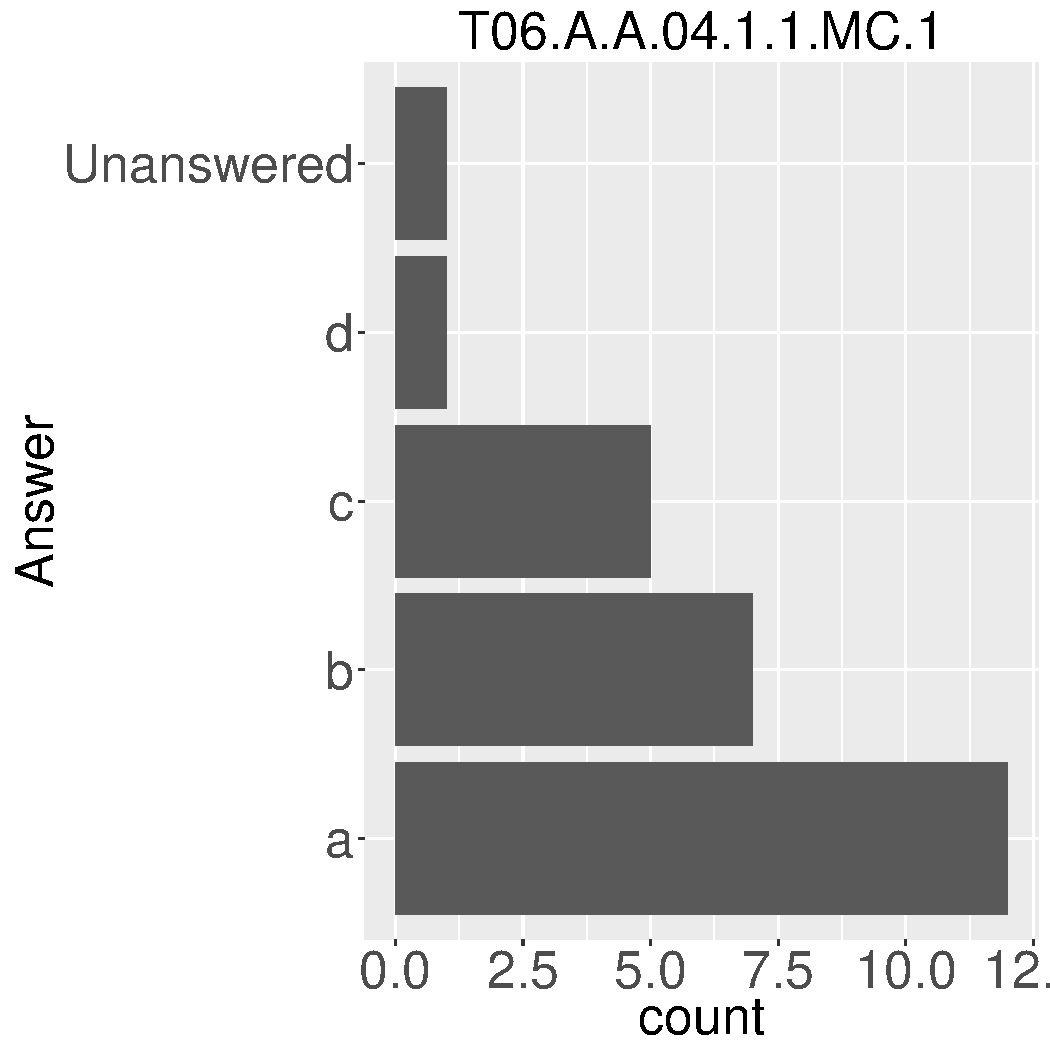
\includegraphics[width=.45\linewidth]{Topic06_1_answer} 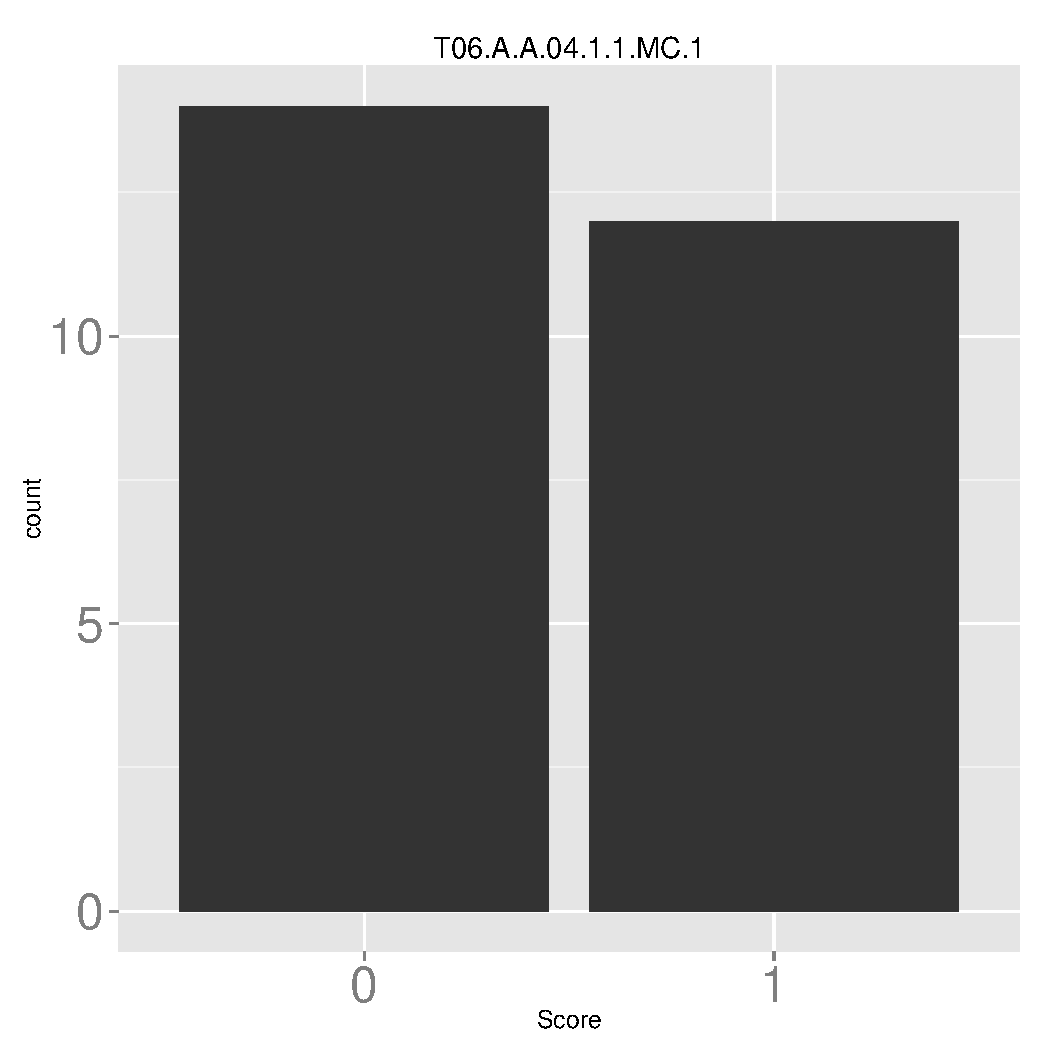
\includegraphics[width=.45\linewidth]{Topic06_1_score} \end{center} 

\begin{center}% latex table generated in R 3.2.2 by xtable 1.8-0 package
% Mon Nov 23 01:15:48 2015
\begin{tabular}{lr}
  \hline
Answer & Count \\ 
  \hline
a &  12 \\ 
  b &   7 \\ 
  c &   5 \\ 
  d &   1 \\ 
  Unanswered &   1 \\ 
   \hline
\end{tabular}
~~~~~~~~% latex table generated in R 3.2.2 by xtable 1.8-0 package
% Mon Nov 23 01:15:48 2015
\begin{tabular}{lr}
  \hline
Summary & Value \\ 
  \hline
Mean & 0.46 \\ 
  Std.dev & 0.51 \\ 
  Min & 0.00 \\ 
  Median & 0.00 \\ 
  Max & 1.00 \\ 
   \hline
\end{tabular}
\end{center}\newpage\marginnote{

 The z-score for a particular observation is z = 0.4. This means the observation is



*a. 0.4 standard deviations above the mean.



b. 0.4 standard deviations below the mean.



c. 0.4 units above the mean.



d. 0.4 units below the mean. 

}\pdfbookmark[2]{T06.A.A.04.1.1.MC.2}{T06.A.A.04.1.1.MC.2} (2) Question "T06.A.A.04.1.1.MC.2" is given on the right. This question was selected from the question set with a frequency of 0.25. The question was administered to 24 out of the total of 100 students. The average score was 0.54 out of 1.

 (Back to the question summary Table \ref{tab:summary_question}.)

\begin{center} 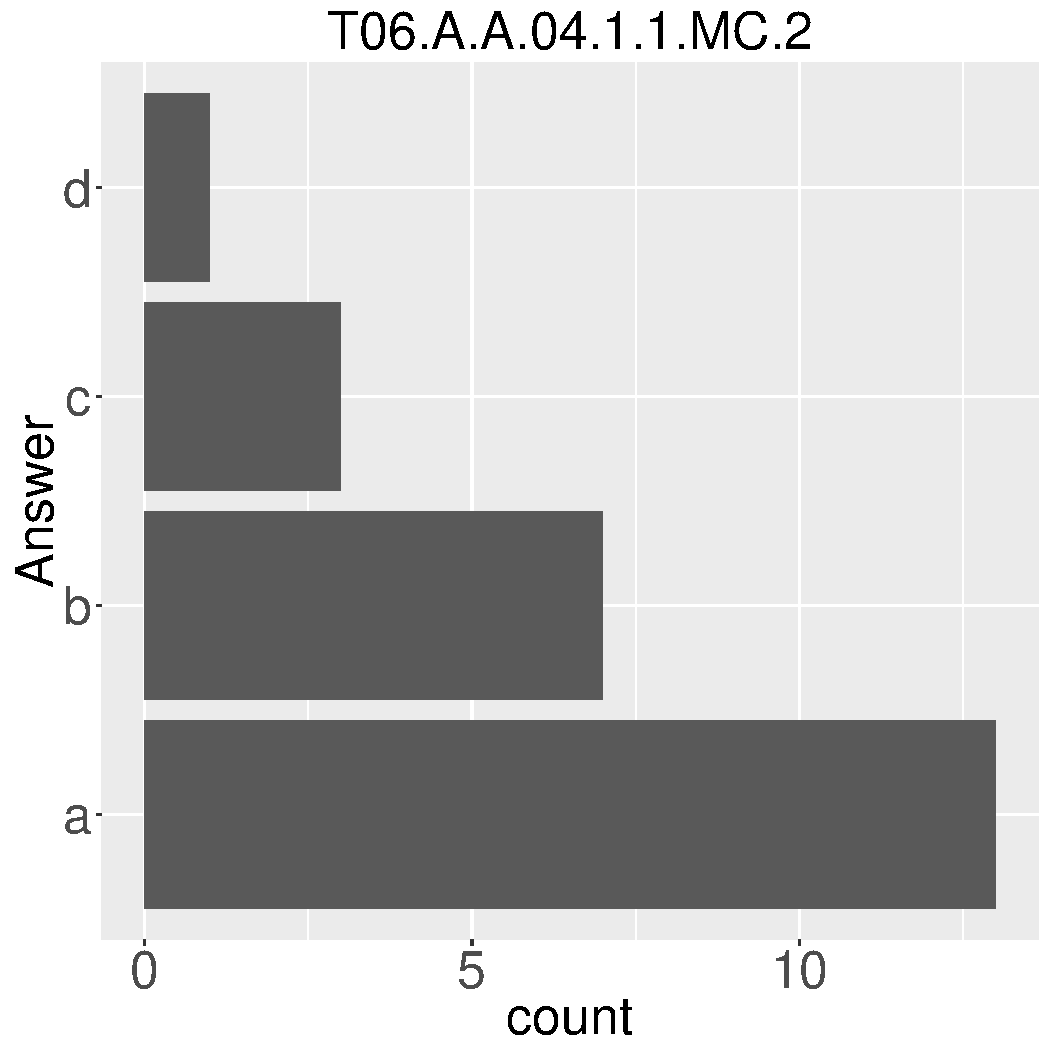
\includegraphics[width=.45\linewidth]{Topic06_2_answer} 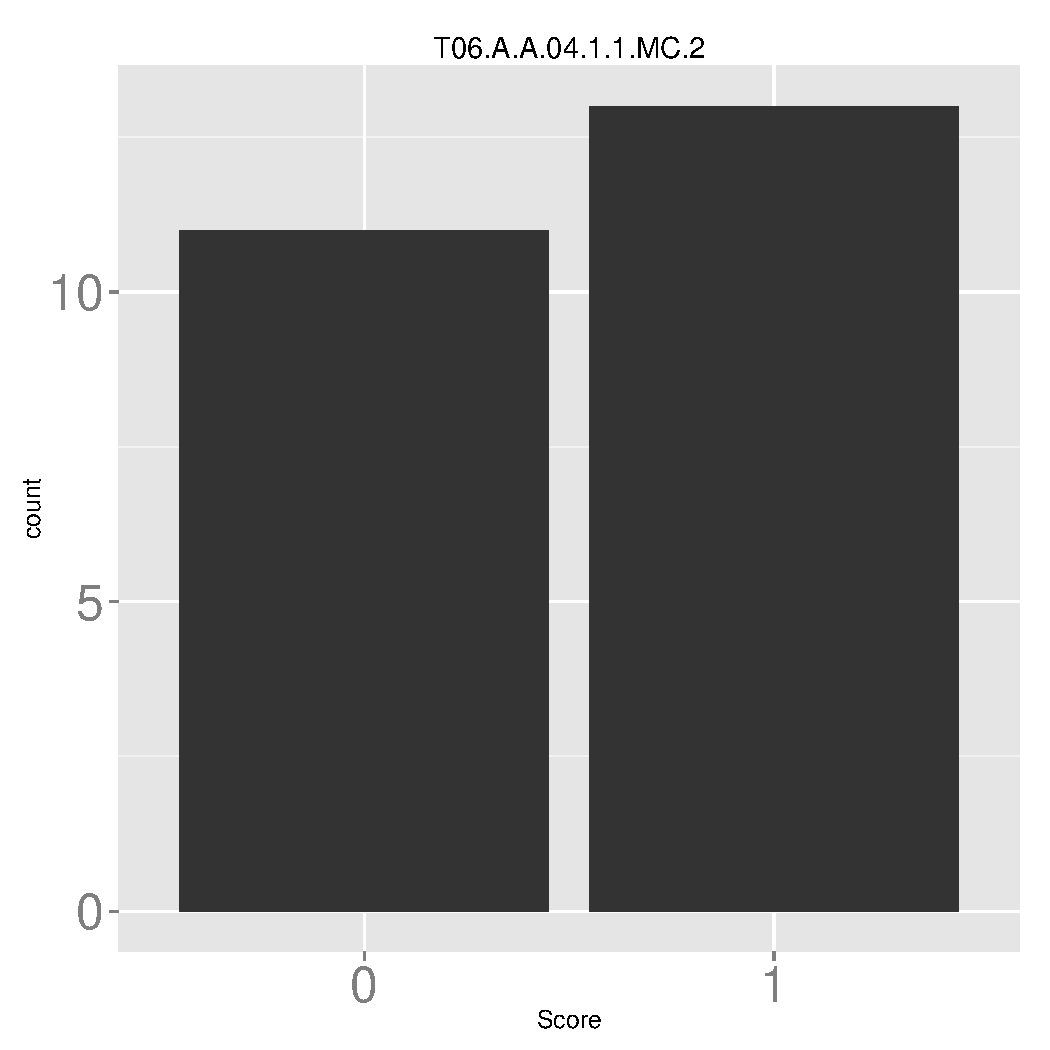
\includegraphics[width=.45\linewidth]{Topic06_2_score} \end{center} 

\begin{center}% latex table generated in R 3.2.2 by xtable 1.8-0 package
% Mon Nov 23 01:15:48 2015
\begin{tabular}{lr}
  \hline
Answer & Count \\ 
  \hline
a &  13 \\ 
  b &   7 \\ 
  c &   3 \\ 
  d &   1 \\ 
   \hline
\end{tabular}
~~~~~~~~% latex table generated in R 3.2.2 by xtable 1.8-0 package
% Mon Nov 23 01:15:48 2015
\begin{tabular}{lr}
  \hline
Summary & Value \\ 
  \hline
Mean & 0.54 \\ 
  Std.dev & 0.51 \\ 
  Min & 0.00 \\ 
  Median & 1.00 \\ 
  Max & 1.00 \\ 
   \hline
\end{tabular}
\end{center}\newpage\marginnote{

 The z-score for a particular observation is z = 2.3. This means the observation is



*a. 2.3 standard deviations above the mean.



b. 2.3 standard deviations below the mean.



c. 2.3 units above the mean.



d. 2.3 units below the mean. 

}\pdfbookmark[2]{T06.A.A.04.1.1.MC.3}{T06.A.A.04.1.1.MC.3} (3) Question "T06.A.A.04.1.1.MC.3" is given on the right. This question was selected from the question set with a frequency of 0.25. The question was administered to 22 out of the total of 100 students. The average score was 0.36 out of 1.

 (Back to the question summary Table \ref{tab:summary_question}.)

\begin{center} 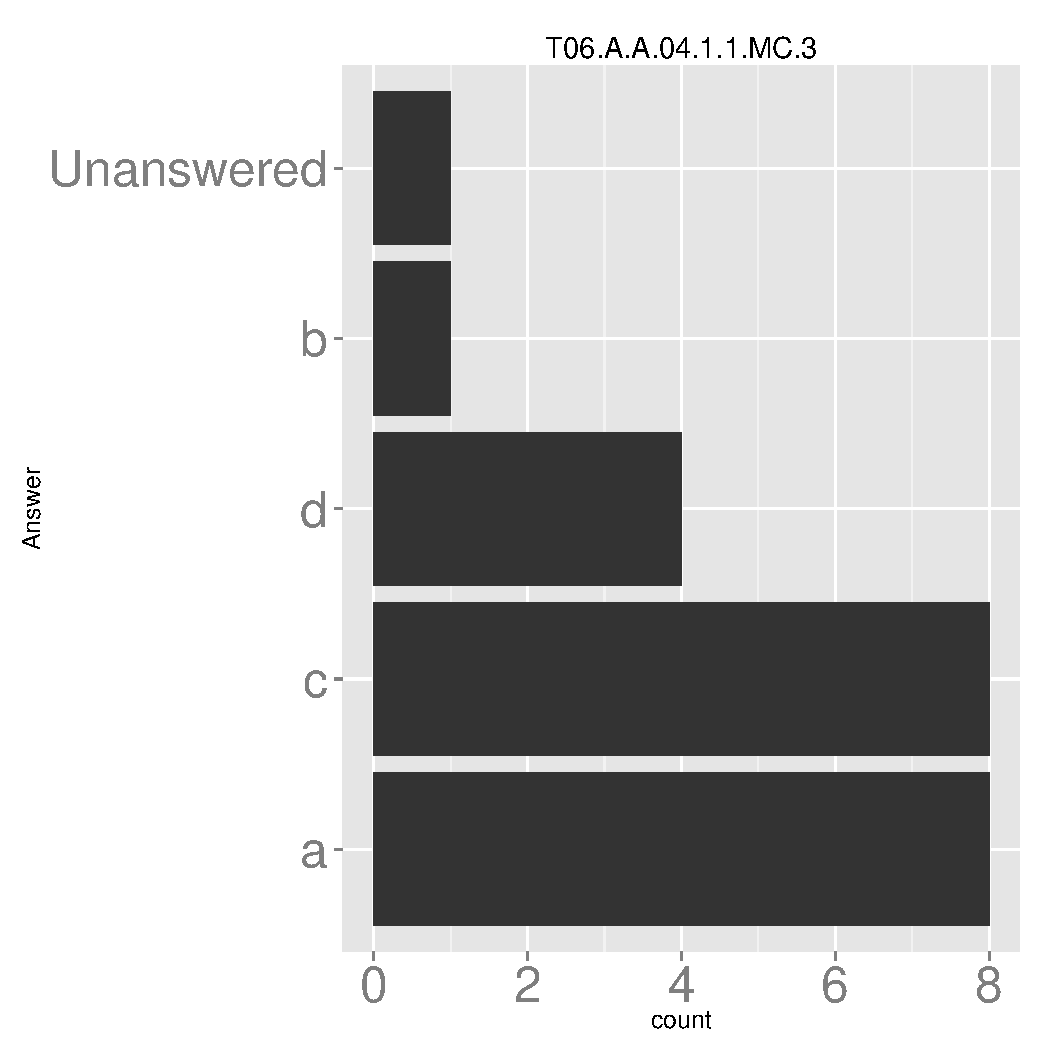
\includegraphics[width=.45\linewidth]{Topic06_3_answer} 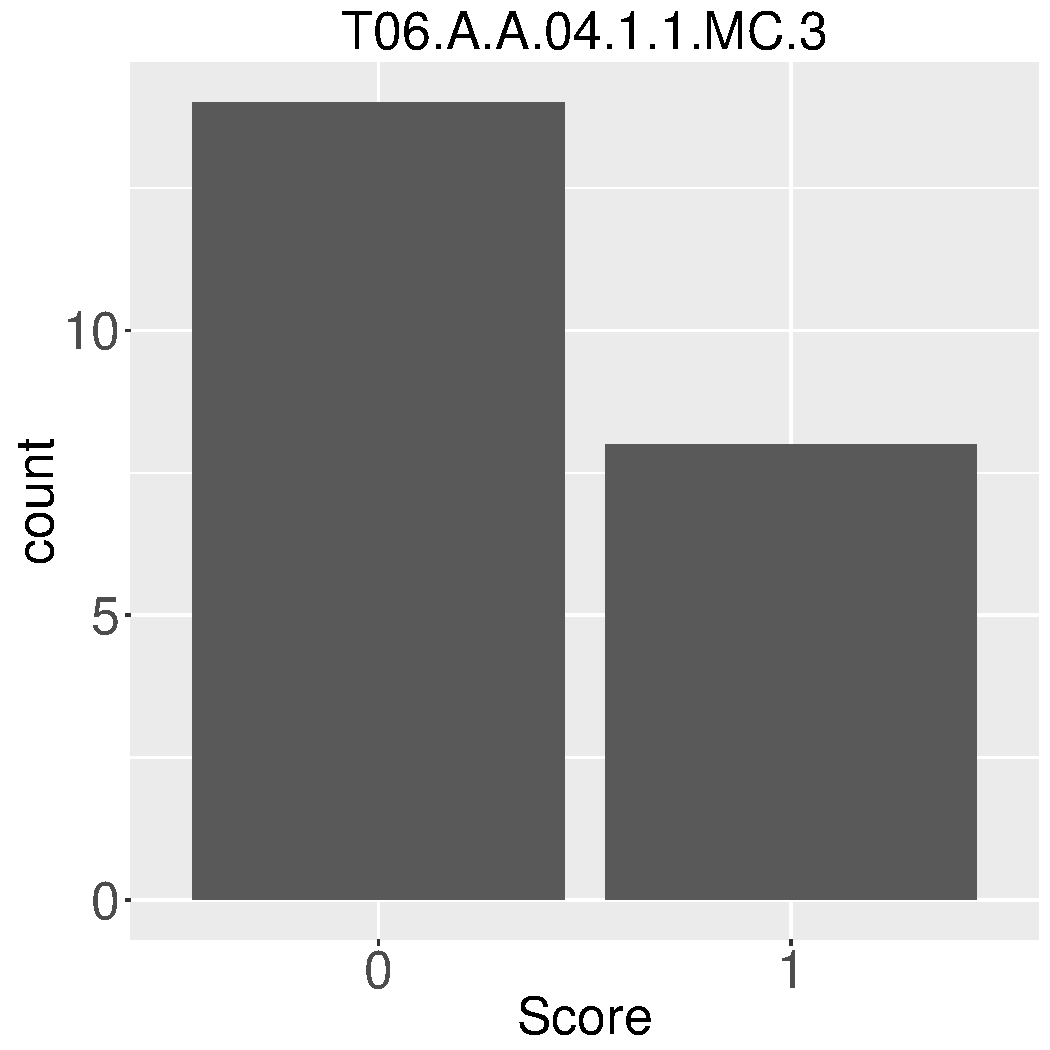
\includegraphics[width=.45\linewidth]{Topic06_3_score} \end{center} 

\begin{center}% latex table generated in R 3.2.2 by xtable 1.8-0 package
% Mon Nov 23 01:15:49 2015
\begin{tabular}{lr}
  \hline
Answer & Count \\ 
  \hline
a &   8 \\ 
  c &   8 \\ 
  d &   4 \\ 
  b &   1 \\ 
  Unanswered &   1 \\ 
   \hline
\end{tabular}
~~~~~~~~% latex table generated in R 3.2.2 by xtable 1.8-0 package
% Mon Nov 23 01:15:49 2015
\begin{tabular}{lr}
  \hline
Summary & Value \\ 
  \hline
Mean & 0.36 \\ 
  Std.dev & 0.49 \\ 
  Min & 0.00 \\ 
  Median & 0.00 \\ 
  Max & 1.00 \\ 
   \hline
\end{tabular}
\end{center}\newpage\marginnote{

 The z-score for a particular observation is z = 3.4. This means the observation is



*a. 3.4 standard deviations above the mean.



b. 3.4 standard deviations below the mean.



c. 3.4 units above the mean.



d. 3.4 units below the mean. 

}\pdfbookmark[2]{T06.A.A.04.1.1.MC.4}{T06.A.A.04.1.1.MC.4} (4) Question "T06.A.A.04.1.1.MC.4" is given on the right. This question was selected from the question set with a frequency of 0.25. The question was administered to 28 out of the total of 100 students. The average score was 0.46 out of 1.

 (Back to the question summary Table \ref{tab:summary_question}.)

\begin{center} 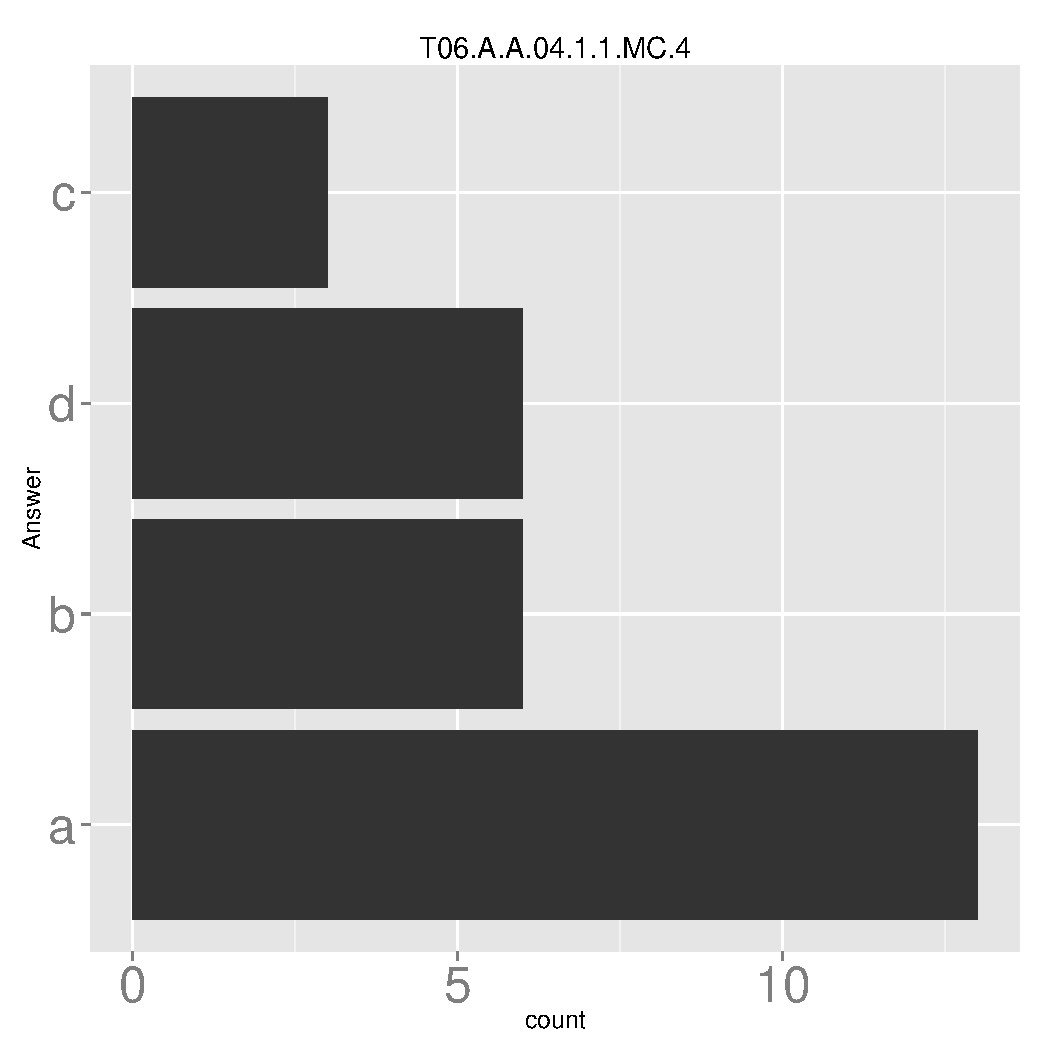
\includegraphics[width=.45\linewidth]{Topic06_4_answer} 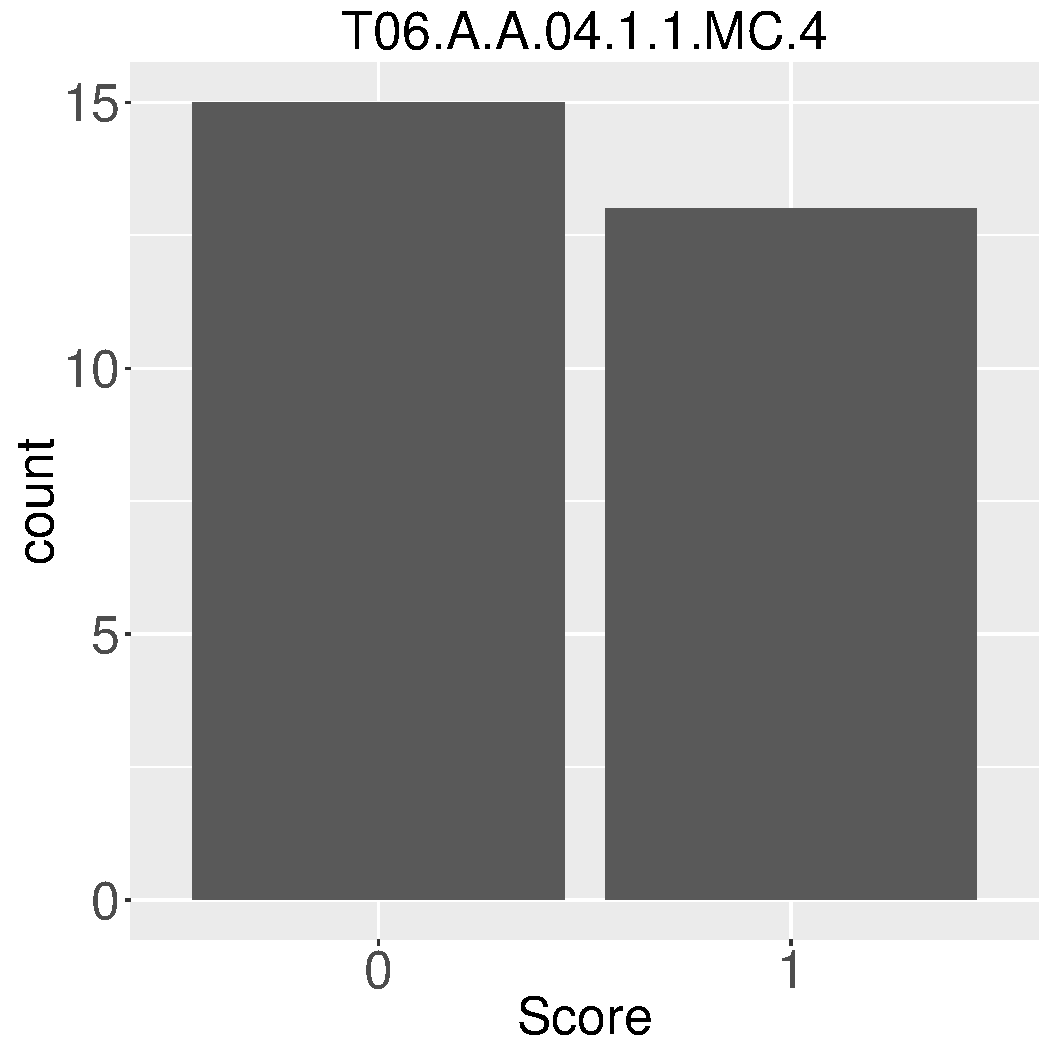
\includegraphics[width=.45\linewidth]{Topic06_4_score} \end{center} 

\begin{center}% latex table generated in R 3.2.2 by xtable 1.8-0 package
% Mon Nov 23 01:15:49 2015
\begin{tabular}{lr}
  \hline
Answer & Count \\ 
  \hline
a &  13 \\ 
  b &   6 \\ 
  d &   6 \\ 
  c &   3 \\ 
   \hline
\end{tabular}
~~~~~~~~% latex table generated in R 3.2.2 by xtable 1.8-0 package
% Mon Nov 23 01:15:49 2015
\begin{tabular}{lr}
  \hline
Summary & Value \\ 
  \hline
Mean & 0.46 \\ 
  Std.dev & 0.51 \\ 
  Min & 0.00 \\ 
  Median & 0.00 \\ 
  Max & 1.00 \\ 
   \hline
\end{tabular}
\end{center}\newpage\marginnote{

 The z-score for a particular observation is z = -1.2. This means the observation is



a. 1.2 standard deviations above the mean.



*b. 1.2 standard deviations below the mean.



c. 1.2 units above the mean.



d. 1.2 units below the mean. 

}\pdfbookmark[2]{T06.A.B.04.1.1.MC.1}{T06.A.B.04.1.1.MC.1} (5) Question "T06.A.B.04.1.1.MC.1" is given on the right. This question was selected from the question set with a frequency of 0.25. The question was administered to 32 out of the total of 100 students. The average score was 0.5 out of 1.

 (Back to the question summary Table \ref{tab:summary_question}.)

\begin{center} 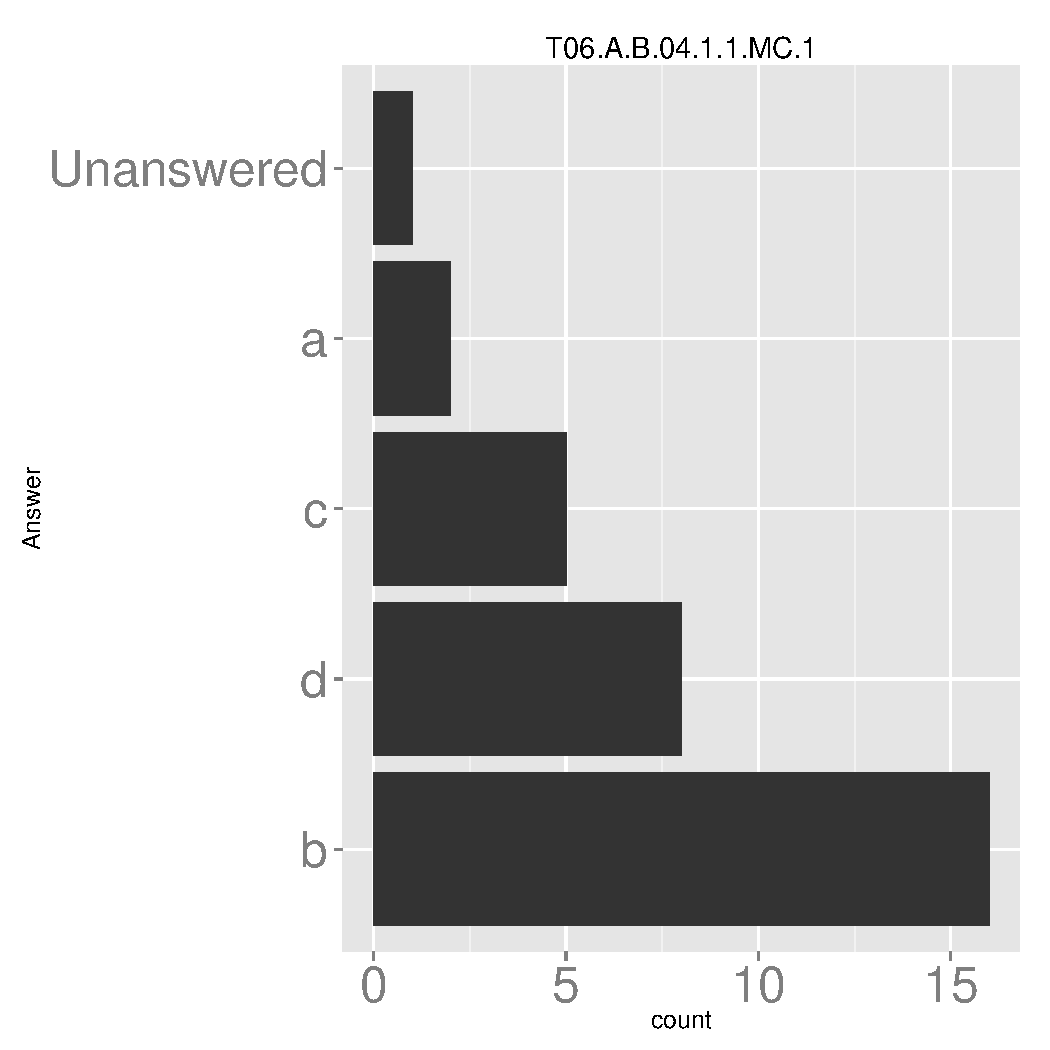
\includegraphics[width=.45\linewidth]{Topic06_5_answer} 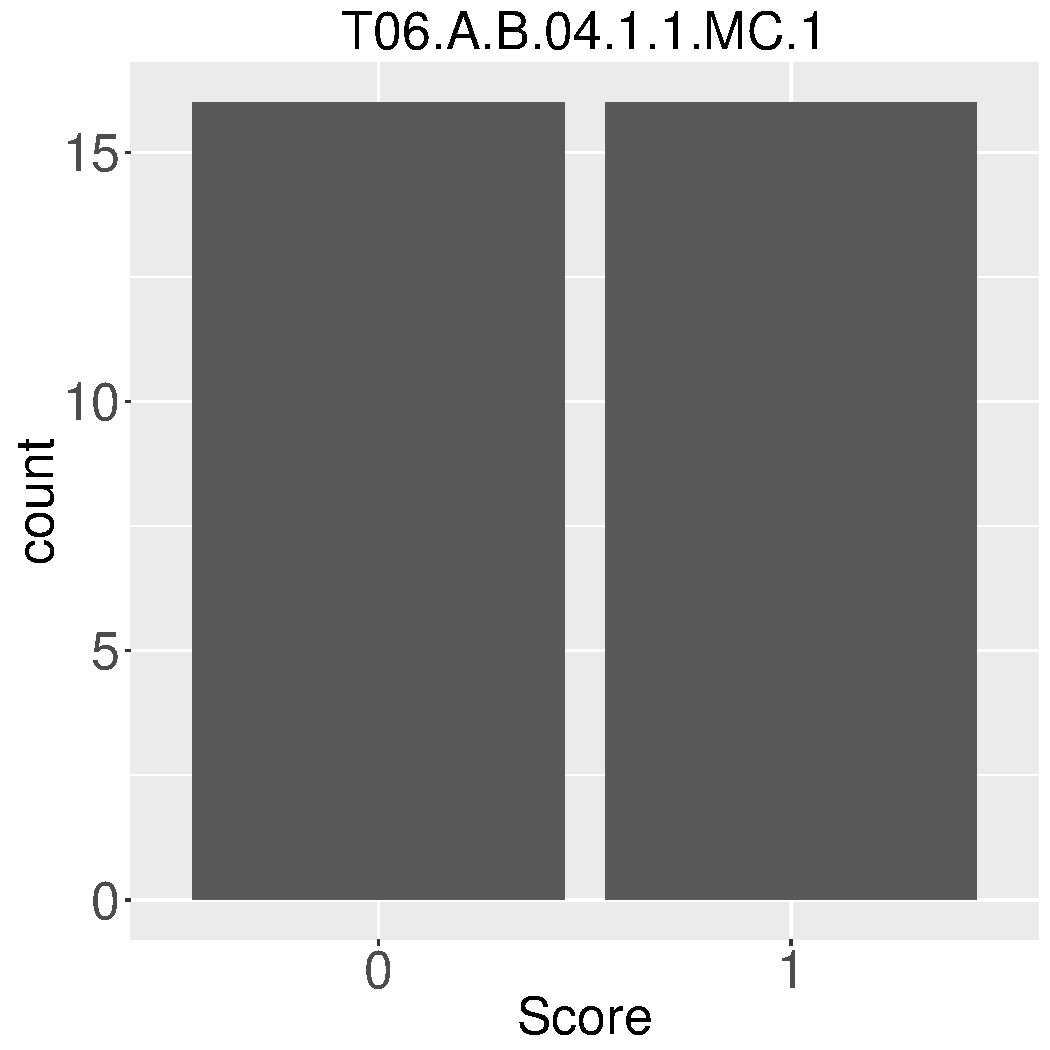
\includegraphics[width=.45\linewidth]{Topic06_5_score} \end{center} 

\begin{center}% latex table generated in R 3.2.2 by xtable 1.8-0 package
% Mon Nov 23 01:15:50 2015
\begin{tabular}{lr}
  \hline
Answer & Count \\ 
  \hline
b &  16 \\ 
  d &   8 \\ 
  c &   5 \\ 
  a &   2 \\ 
  Unanswered &   1 \\ 
   \hline
\end{tabular}
~~~~~~~~% latex table generated in R 3.2.2 by xtable 1.8-0 package
% Mon Nov 23 01:15:50 2015
\begin{tabular}{lr}
  \hline
Summary & Value \\ 
  \hline
Mean & 0.50 \\ 
  Std.dev & 0.51 \\ 
  Min & 0.00 \\ 
  Median & 0.50 \\ 
  Max & 1.00 \\ 
   \hline
\end{tabular}
\end{center}\newpage\marginnote{

 The z-score for a particular observation is z = -0.8. This means the observation is



a. 0.8 standard deviations above the mean.



*b. 0.8 standard deviations below the mean.



c. 0.8 units above the mean.



d. 0.8 units below the mean. 

}\pdfbookmark[2]{T06.A.B.04.1.1.MC.2}{T06.A.B.04.1.1.MC.2} (6) Question "T06.A.B.04.1.1.MC.2" is given on the right. This question was selected from the question set with a frequency of 0.25. The question was administered to 26 out of the total of 100 students. The average score was 0.5 out of 1.

 (Back to the question summary Table \ref{tab:summary_question}.)

\begin{center} 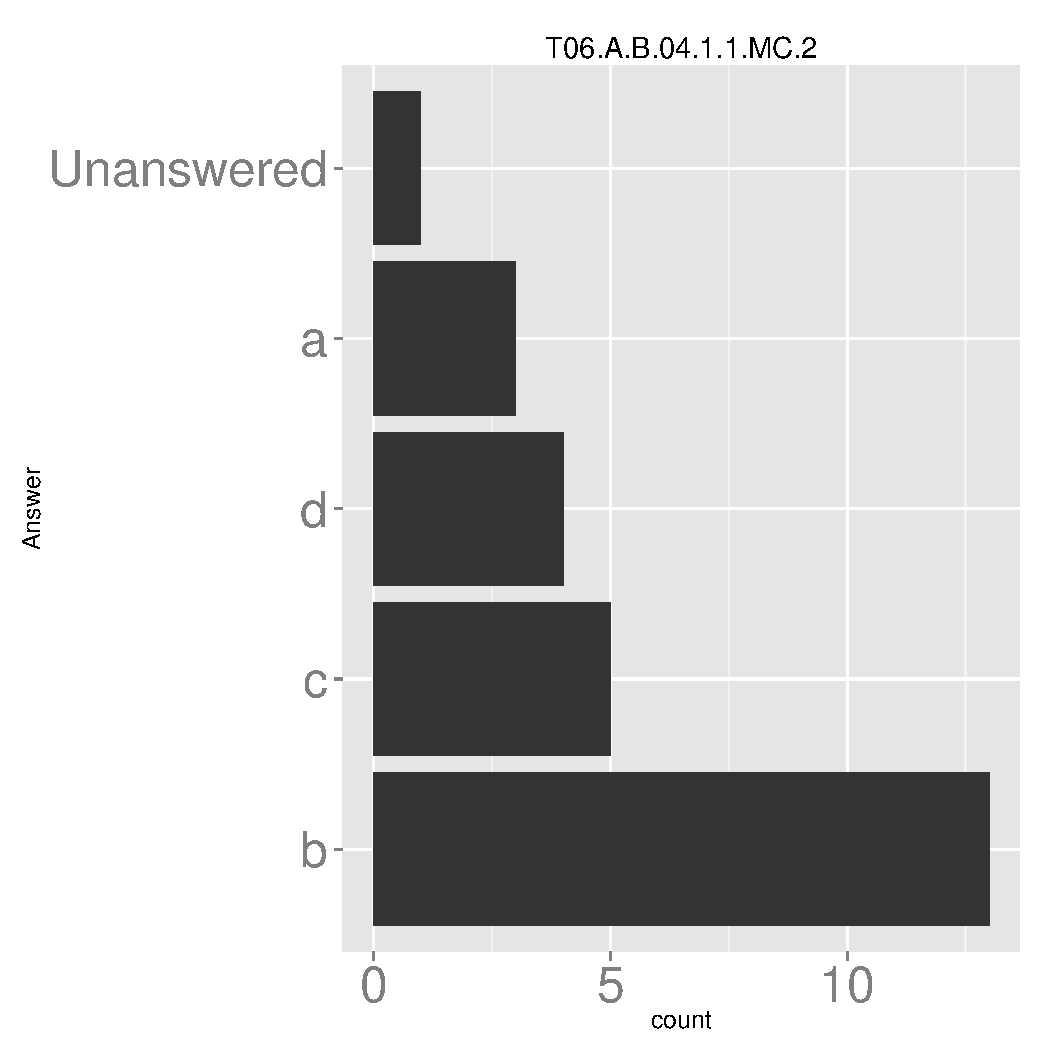
\includegraphics[width=.45\linewidth]{Topic06_6_answer} 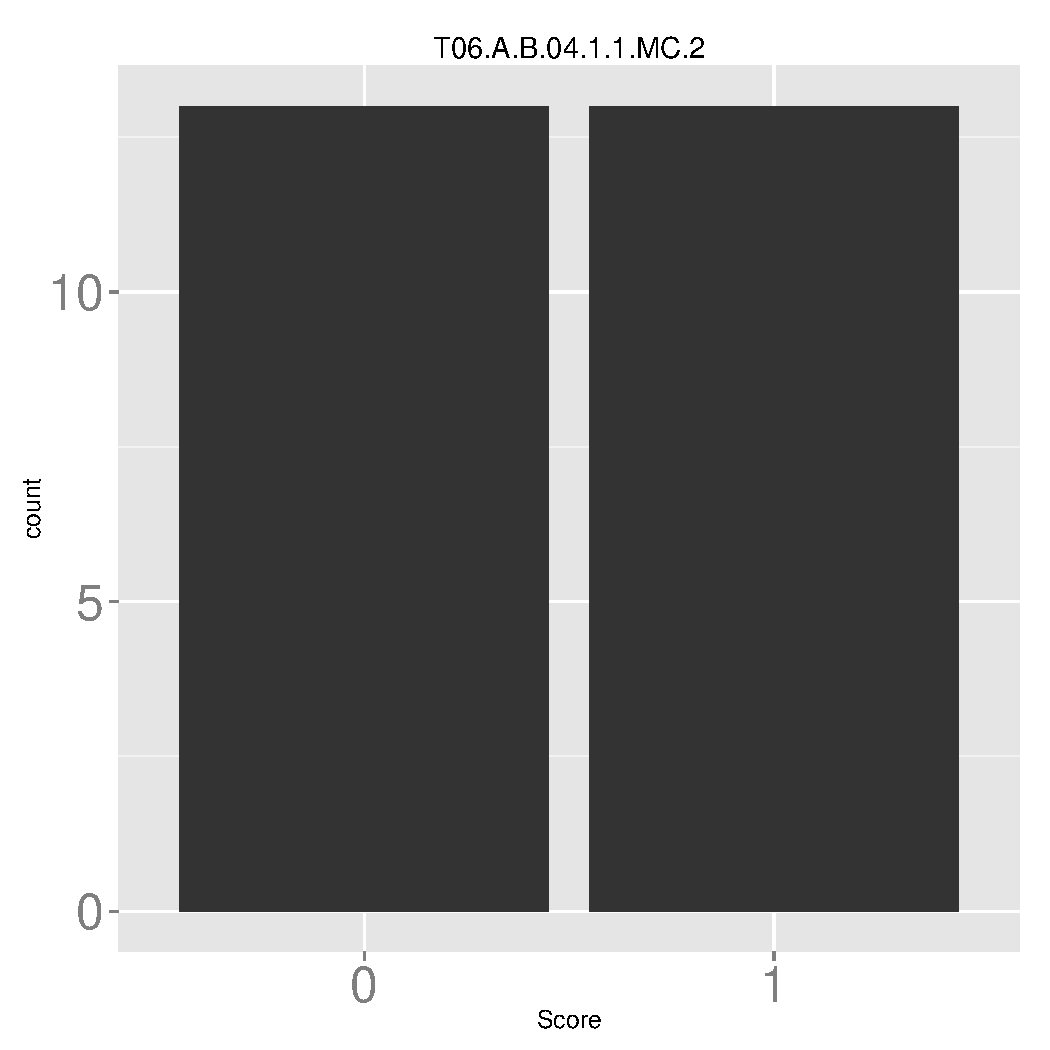
\includegraphics[width=.45\linewidth]{Topic06_6_score} \end{center} 

\begin{center}% latex table generated in R 3.2.2 by xtable 1.8-0 package
% Mon Nov 23 01:15:50 2015
\begin{tabular}{lr}
  \hline
Answer & Count \\ 
  \hline
b &  13 \\ 
  c &   5 \\ 
  d &   4 \\ 
  a &   3 \\ 
  Unanswered &   1 \\ 
   \hline
\end{tabular}
~~~~~~~~% latex table generated in R 3.2.2 by xtable 1.8-0 package
% Mon Nov 23 01:15:50 2015
\begin{tabular}{lr}
  \hline
Summary & Value \\ 
  \hline
Mean & 0.50 \\ 
  Std.dev & 0.51 \\ 
  Min & 0.00 \\ 
  Median & 0.50 \\ 
  Max & 1.00 \\ 
   \hline
\end{tabular}
\end{center}\newpage\marginnote{

 The z-score for a particular observation is z = -2.7. This means the observation is



a. 2.7 standard deviations above the mean.



*b. 2.7 standard deviations below the mean.



c. 2.7 units above the mean.



d. 2.7 units below the mean. 

}\pdfbookmark[2]{T06.A.B.04.1.1.MC.3}{T06.A.B.04.1.1.MC.3} (7) Question "T06.A.B.04.1.1.MC.3" is given on the right. This question was selected from the question set with a frequency of 0.25. The question was administered to 21 out of the total of 100 students. The average score was 0.52 out of 1.

 (Back to the question summary Table \ref{tab:summary_question}.)

\begin{center} 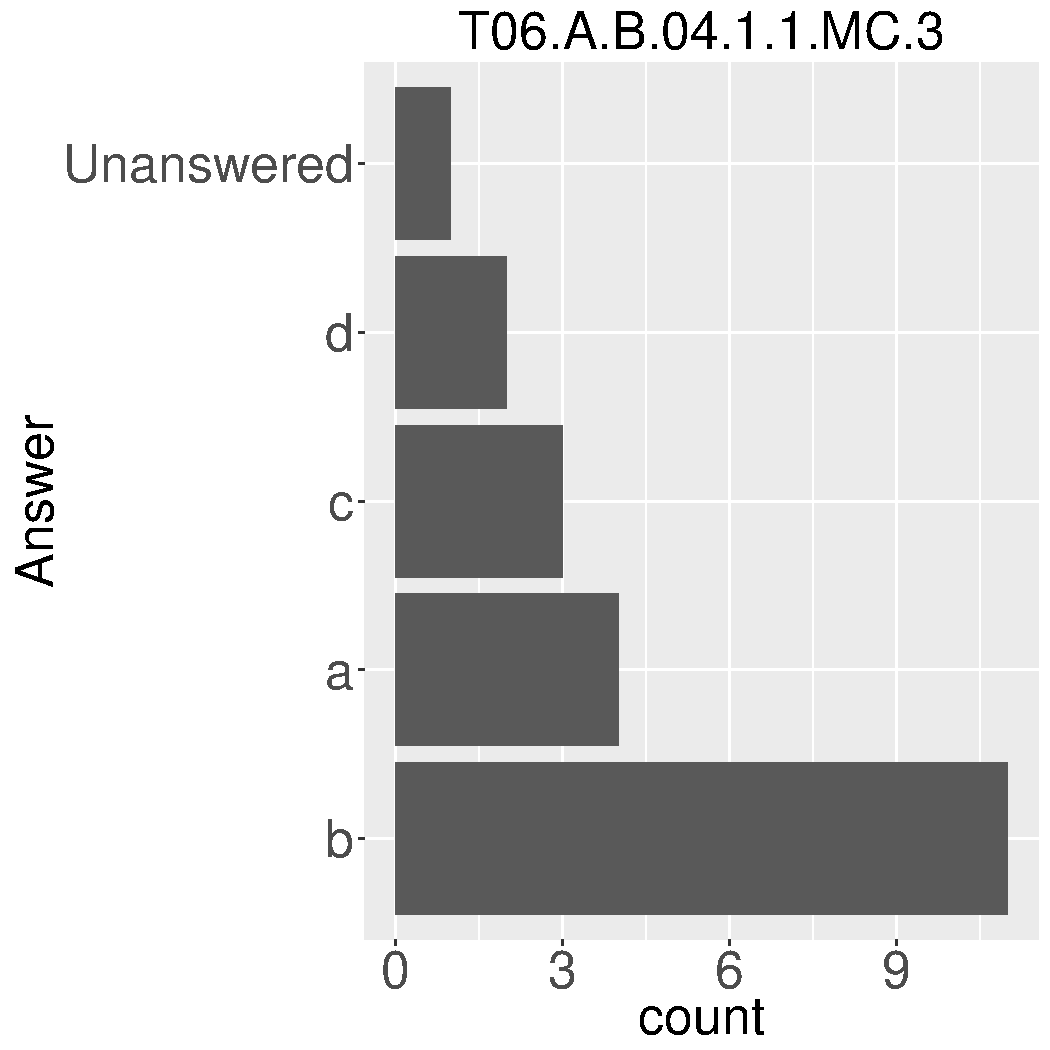
\includegraphics[width=.45\linewidth]{Topic06_7_answer} 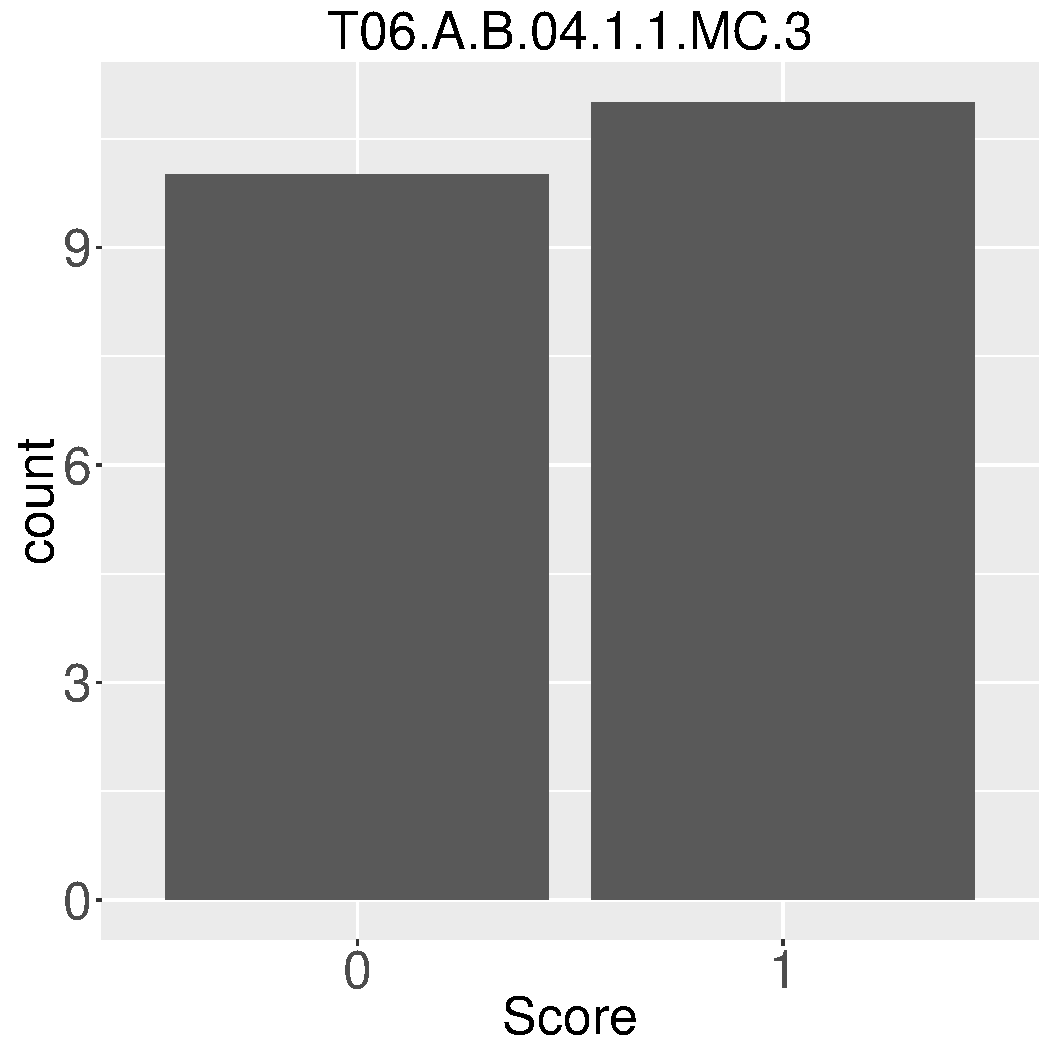
\includegraphics[width=.45\linewidth]{Topic06_7_score} \end{center} 

\begin{center}% latex table generated in R 3.2.2 by xtable 1.8-0 package
% Mon Nov 23 01:15:50 2015
\begin{tabular}{lr}
  \hline
Answer & Count \\ 
  \hline
b &  11 \\ 
  a &   4 \\ 
  c &   3 \\ 
  d &   2 \\ 
  Unanswered &   1 \\ 
   \hline
\end{tabular}
~~~~~~~~% latex table generated in R 3.2.2 by xtable 1.8-0 package
% Mon Nov 23 01:15:50 2015
\begin{tabular}{lr}
  \hline
Summary & Value \\ 
  \hline
Mean & 0.52 \\ 
  Std.dev & 0.51 \\ 
  Min & 0.00 \\ 
  Median & 1.00 \\ 
  Max & 1.00 \\ 
   \hline
\end{tabular}
\end{center}\newpage\marginnote{

 The z-score for a particular observation is z = -3.1. This means the observation is



a. 3.1 standard deviations above the mean.



*b. 3.1 standard deviations below the mean.



c. 3.1 units above the mean.



d. 3.1 units below the mean. 

}\pdfbookmark[2]{T06.A.B.04.1.1.MC.4}{T06.A.B.04.1.1.MC.4} (8) Question "T06.A.B.04.1.1.MC.4" is given on the right. This question was selected from the question set with a frequency of 0.25. The question was administered to 21 out of the total of 100 students. The average score was 0.52 out of 1.

 (Back to the question summary Table \ref{tab:summary_question}.)

\begin{center} 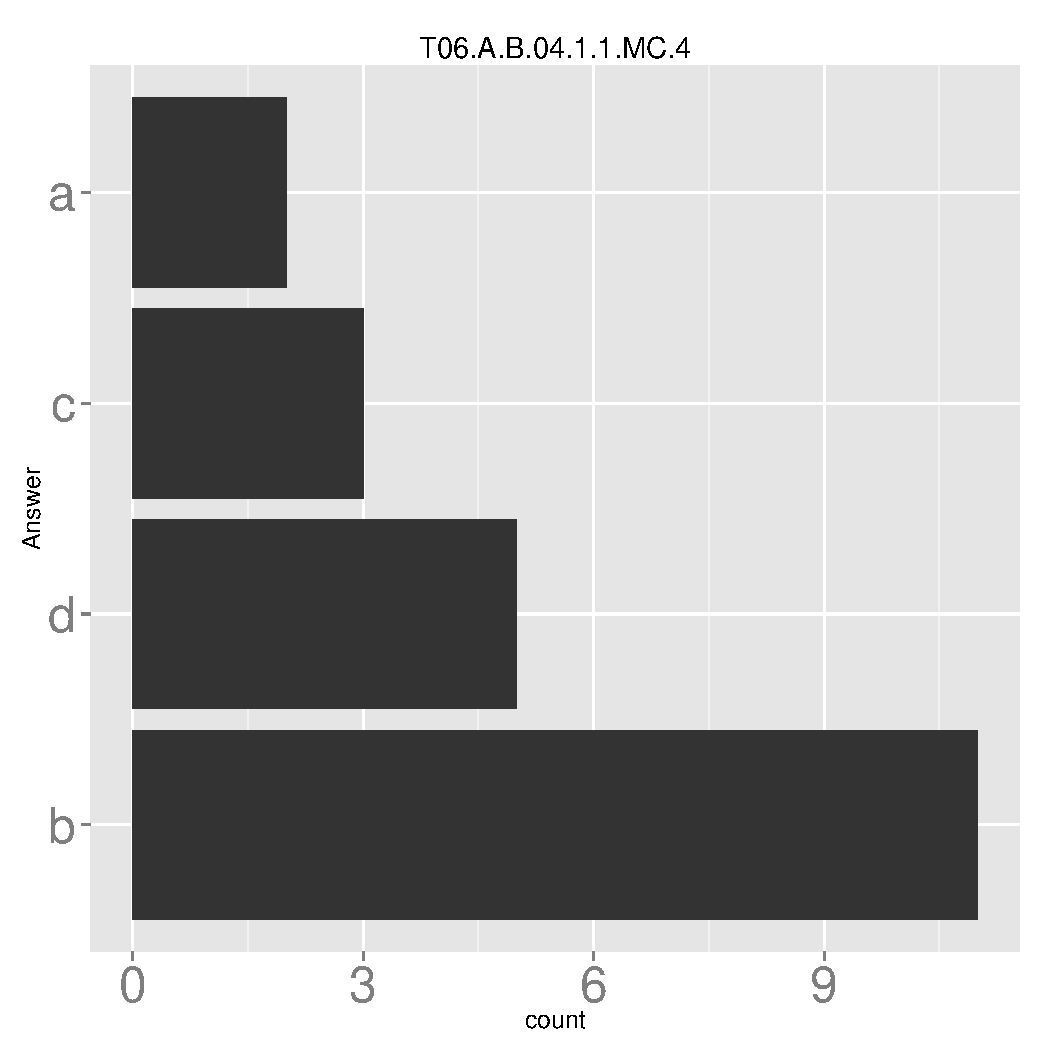
\includegraphics[width=.45\linewidth]{Topic06_8_answer} 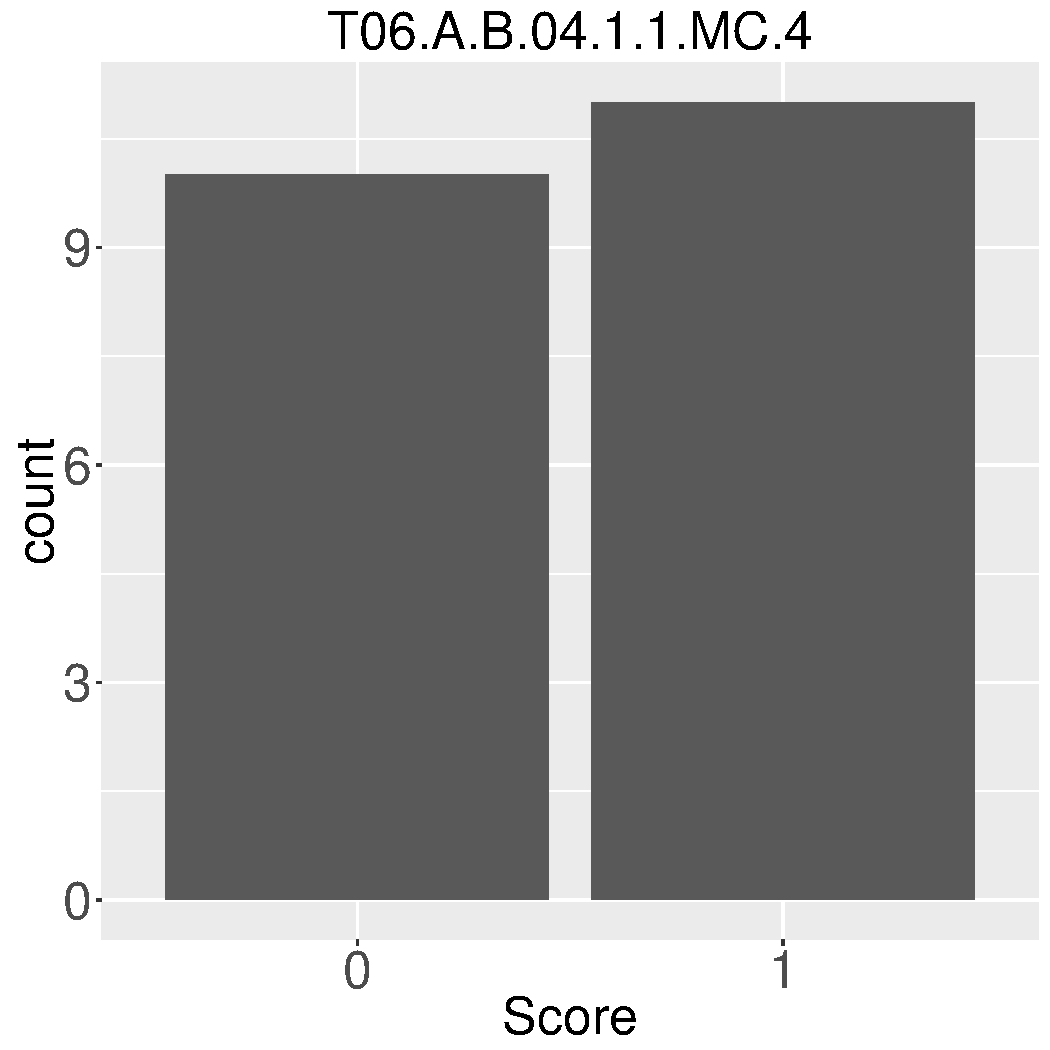
\includegraphics[width=.45\linewidth]{Topic06_8_score} \end{center} 

\begin{center}% latex table generated in R 3.2.2 by xtable 1.8-0 package
% Mon Nov 23 01:15:51 2015
\begin{tabular}{lr}
  \hline
Answer & Count \\ 
  \hline
b &  11 \\ 
  d &   5 \\ 
  c &   3 \\ 
  a &   2 \\ 
   \hline
\end{tabular}
~~~~~~~~% latex table generated in R 3.2.2 by xtable 1.8-0 package
% Mon Nov 23 01:15:51 2015
\begin{tabular}{lr}
  \hline
Summary & Value \\ 
  \hline
Mean & 0.52 \\ 
  Std.dev & 0.51 \\ 
  Min & 0.00 \\ 
  Median & 1.00 \\ 
  Max & 1.00 \\ 
   \hline
\end{tabular}
\end{center}\newpage\marginnote{

 In a sample of 25 male newborns, the mean birth weight was 3.4 kg and the standard deviation was 0.35 kg.



The z-score for a birth weight of 4.5 kg is \_\_\_\_\_\_\_\_\_\_. Round your answer to 2 decimal places.



Correct Answer(s):



a. 3.14



b. 3.15



c. 3.13 

}\pdfbookmark[2]{T06.A.C.04.1.1.FB.1}{T06.A.C.04.1.1.FB.1} (9) Question "T06.A.C.04.1.1.FB.1" is given on the right. This question was selected from the question set with a frequency of 0.25. The question was administered to 23 out of the total of 100 students. The average score was 0 out of 1.

 (Back to the question summary Table \ref{tab:summary_question}.)

\begin{center} 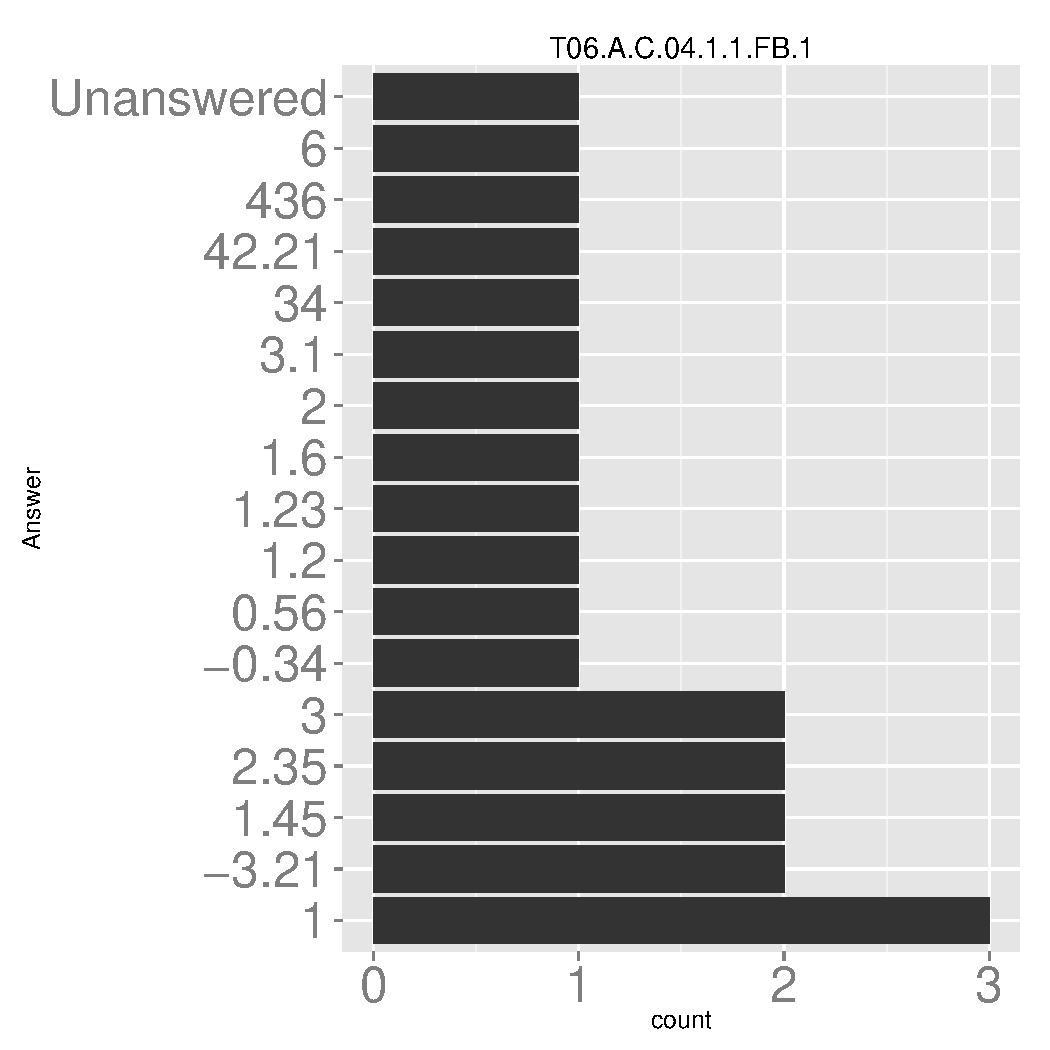
\includegraphics[width=.45\linewidth]{Topic06_9_answer} 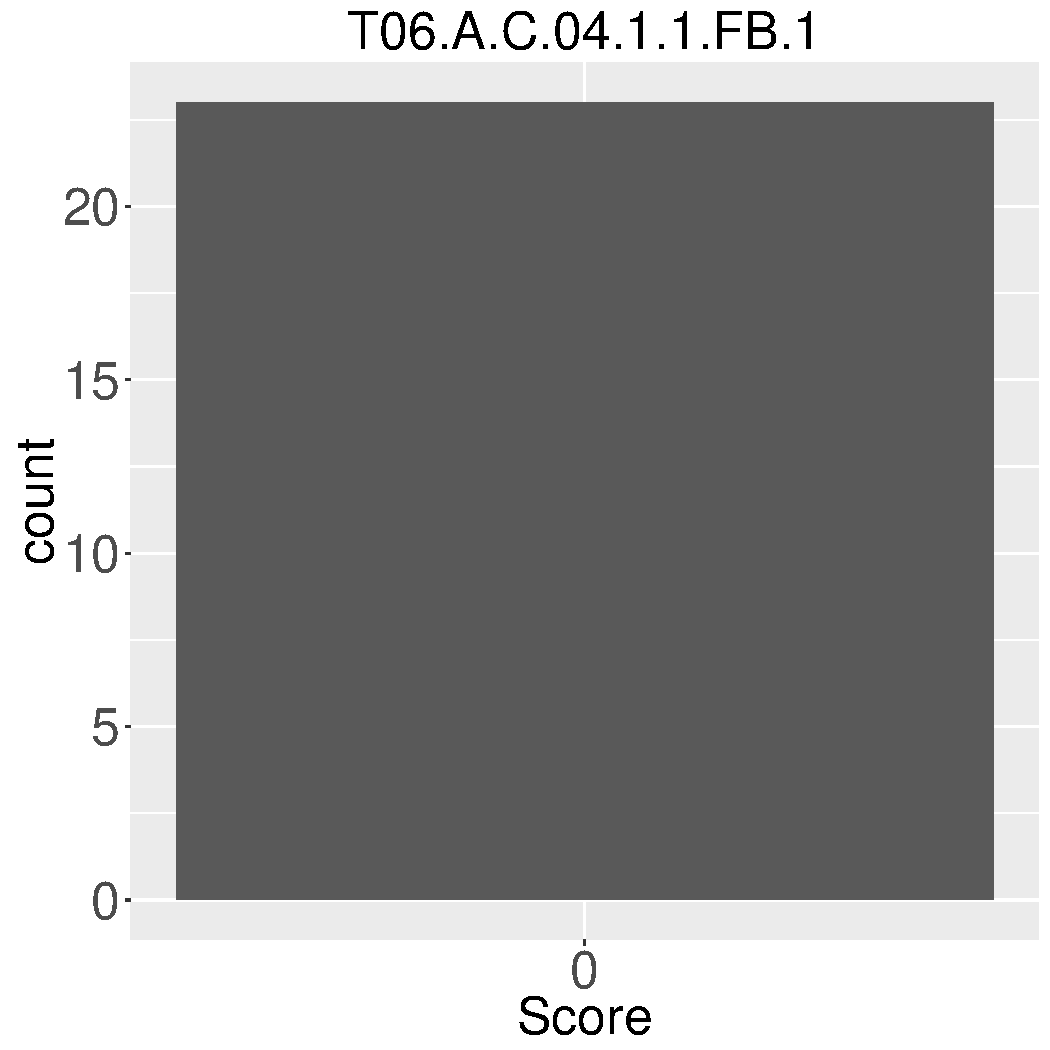
\includegraphics[width=.45\linewidth]{Topic06_9_score} \end{center} 

\begin{center}% latex table generated in R 3.2.2 by xtable 1.8-0 package
% Mon Nov 23 01:15:51 2015
\begin{tabular}{lr}
  \hline
Answer & Count \\ 
  \hline
1 &   3 \\ 
  -3.21 &   2 \\ 
  1.45 &   2 \\ 
  2.35 &   2 \\ 
  3 &   2 \\ 
  -0.34 &   1 \\ 
  0.56 &   1 \\ 
  1.2 &   1 \\ 
  1.23 &   1 \\ 
  1.6 &   1 \\ 
  2 &   1 \\ 
  3.1 &   1 \\ 
  34 &   1 \\ 
  42.21 &   1 \\ 
  436 &   1 \\ 
  6 &   1 \\ 
  Unanswered &   1 \\ 
   \hline
\end{tabular}
~~~~~~~~% latex table generated in R 3.2.2 by xtable 1.8-0 package
% Mon Nov 23 01:15:51 2015
\begin{tabular}{lr}
  \hline
Summary & Value \\ 
  \hline
Mean & 0.00 \\ 
  Std.dev & 0.00 \\ 
  Min & 0.00 \\ 
  Median & 0.00 \\ 
  Max & 0.00 \\ 
   \hline
\end{tabular}
\end{center}\newpage\marginnote{

 In a sample of 25 male newborns, the mean birth weight was 3.4 kg and the standard deviation was 0.35 kg.



The z-score for a birth weight of 4.0 kg is \_\_\_\_\_\_\_\_\_\_. Round your answer to 2 decimal places.



Correct Answer(s):



a. 1.71



b. 1.72



c. 1.70



d. 1.7 

}\pdfbookmark[2]{T06.A.C.04.1.1.FB.2}{T06.A.C.04.1.1.FB.2} (10) Question "T06.A.C.04.1.1.FB.2" is given on the right. This question was selected from the question set with a frequency of 0.25. The question was administered to 27 out of the total of 100 students. The average score was 0 out of 1.

 (Back to the question summary Table \ref{tab:summary_question}.)

\begin{center} 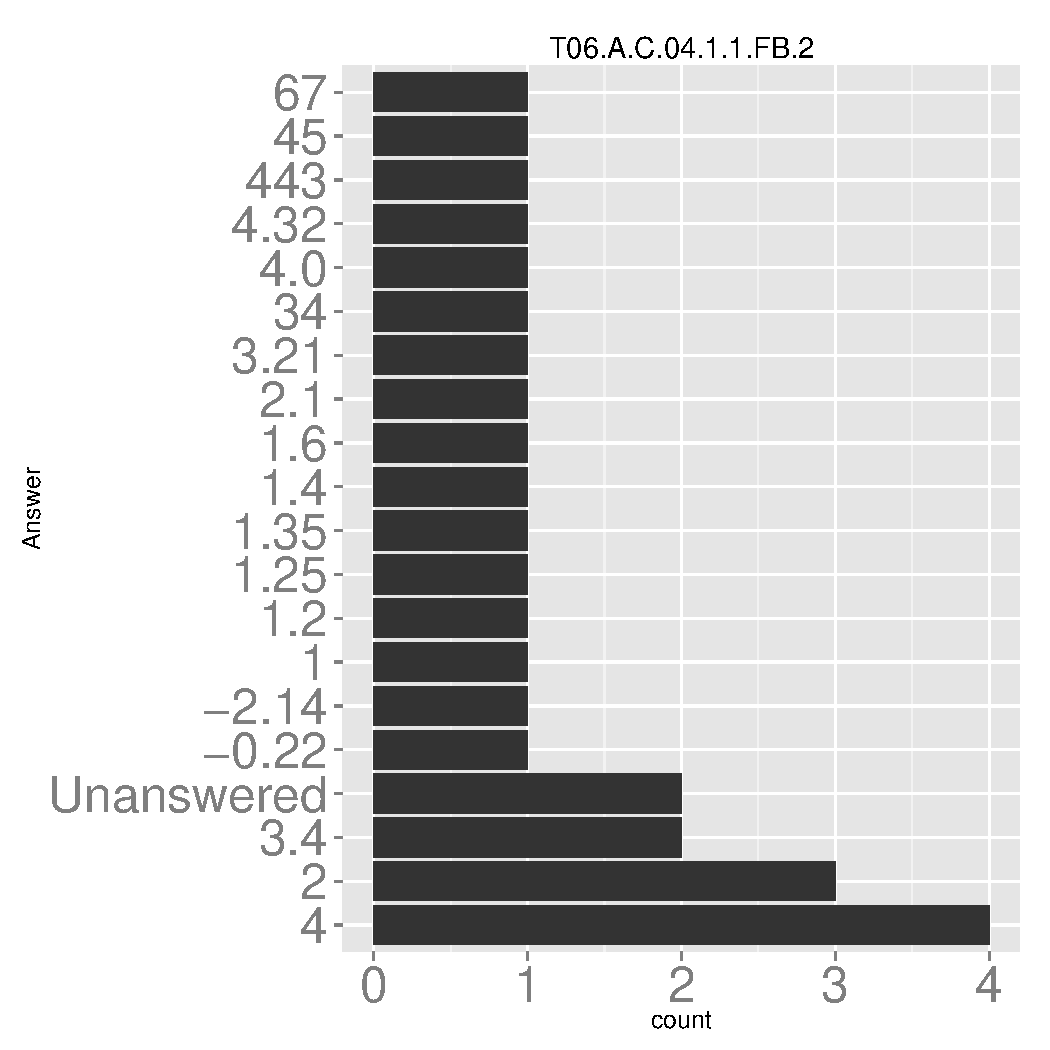
\includegraphics[width=.45\linewidth]{Topic06_10_answer} 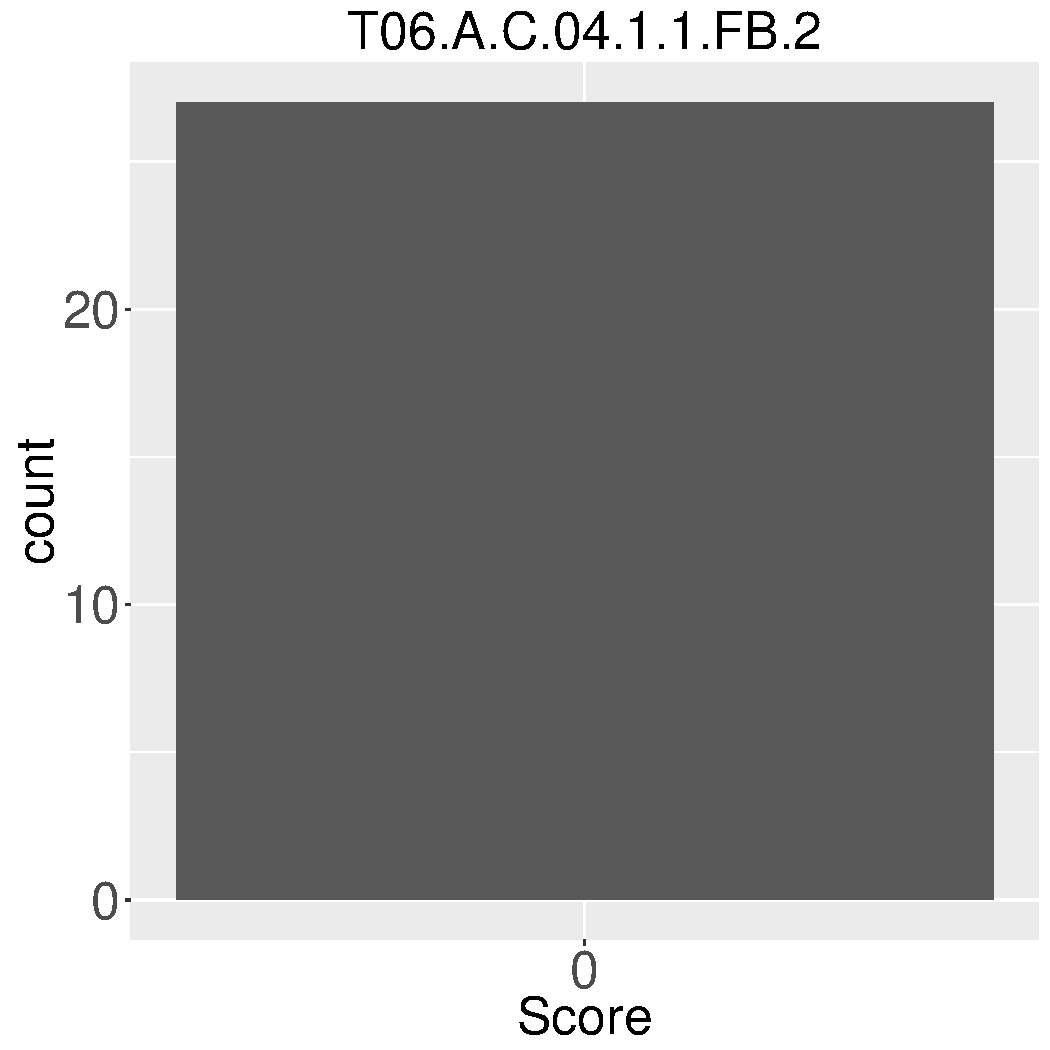
\includegraphics[width=.45\linewidth]{Topic06_10_score} \end{center} 

\begin{center}% latex table generated in R 3.2.2 by xtable 1.8-0 package
% Mon Nov 23 01:15:52 2015
\begin{tabular}{lr}
  \hline
Answer & Count \\ 
  \hline
4 &   4 \\ 
  2 &   3 \\ 
  3.4 &   2 \\ 
  Unanswered &   2 \\ 
  -0.22 &   1 \\ 
  -2.14 &   1 \\ 
  1 &   1 \\ 
  1.2 &   1 \\ 
  1.25 &   1 \\ 
  1.35 &   1 \\ 
  1.4 &   1 \\ 
  1.6 &   1 \\ 
  2.1 &   1 \\ 
  3.21 &   1 \\ 
  34 &   1 \\ 
  4.0 &   1 \\ 
  4.32 &   1 \\ 
  443 &   1 \\ 
  45 &   1 \\ 
  67 &   1 \\ 
   \hline
\end{tabular}
~~~~~~~~% latex table generated in R 3.2.2 by xtable 1.8-0 package
% Mon Nov 23 01:15:52 2015
\begin{tabular}{lr}
  \hline
Summary & Value \\ 
  \hline
Mean & 0.00 \\ 
  Std.dev & 0.00 \\ 
  Min & 0.00 \\ 
  Median & 0.00 \\ 
  Max & 0.00 \\ 
   \hline
\end{tabular}
\end{center}\newpage\marginnote{

 In a sample of 25 male newborns, the mean birth weight was 3.4 kg and the standard deviation was 0.35 kg.



The z-score for a birth weight of 4.2 kg is \_\_\_\_\_\_\_\_\_\_. Round your answer to 2 decimal places.



Correct Answer(s):



a. 2.28



b. 2.29



c. 2.27 

}\pdfbookmark[2]{T06.A.C.04.1.1.FB.3}{T06.A.C.04.1.1.FB.3} (11) Question "T06.A.C.04.1.1.FB.3" is given on the right. This question was selected from the question set with a frequency of 0.25. The question was administered to 23 out of the total of 100 students. The average score was 0 out of 1.

 (Back to the question summary Table \ref{tab:summary_question}.)

\begin{center} 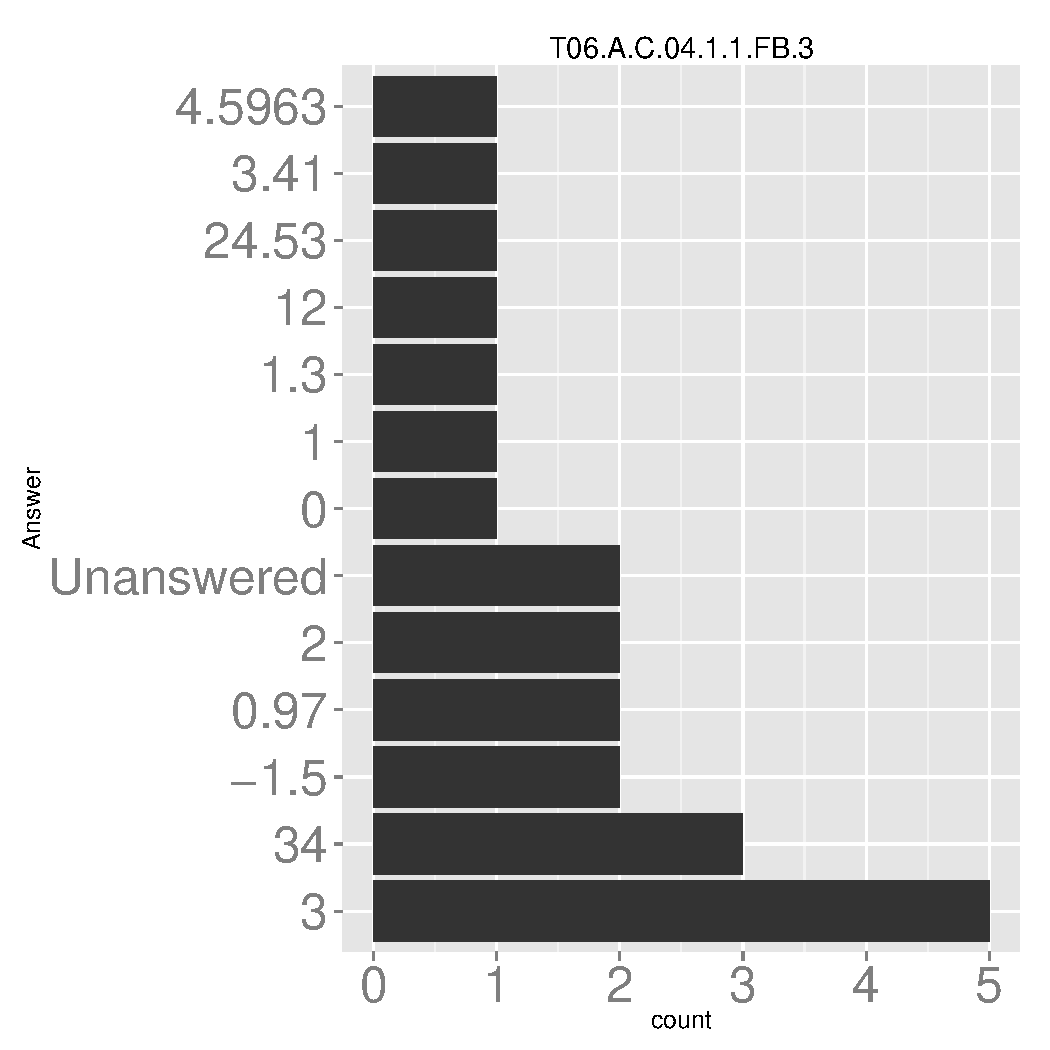
\includegraphics[width=.45\linewidth]{Topic06_11_answer} 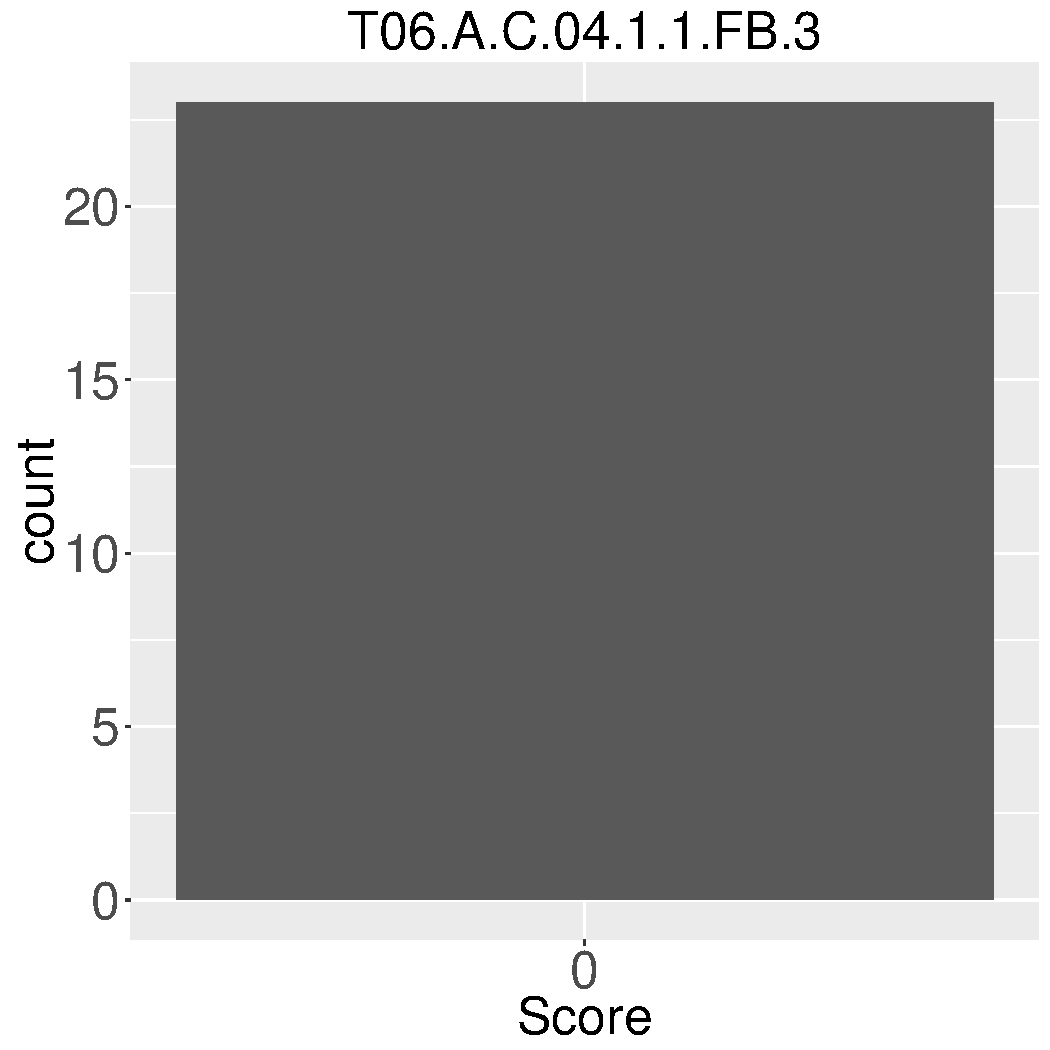
\includegraphics[width=.45\linewidth]{Topic06_11_score} \end{center} 

\begin{center}% latex table generated in R 3.2.2 by xtable 1.8-0 package
% Mon Nov 23 01:15:52 2015
\begin{tabular}{lr}
  \hline
Answer & Count \\ 
  \hline
3 &   5 \\ 
  34 &   3 \\ 
  -1.5 &   2 \\ 
  0.97 &   2 \\ 
  2 &   2 \\ 
  Unanswered &   2 \\ 
  0 &   1 \\ 
  1 &   1 \\ 
  1.3 &   1 \\ 
  12 &   1 \\ 
  24.53 &   1 \\ 
  3.41 &   1 \\ 
  4.5963 &   1 \\ 
   \hline
\end{tabular}
~~~~~~~~% latex table generated in R 3.2.2 by xtable 1.8-0 package
% Mon Nov 23 01:15:52 2015
\begin{tabular}{lr}
  \hline
Summary & Value \\ 
  \hline
Mean & 0.00 \\ 
  Std.dev & 0.00 \\ 
  Min & 0.00 \\ 
  Median & 0.00 \\ 
  Max & 0.00 \\ 
   \hline
\end{tabular}
\end{center}\newpage\marginnote{

 In a sample of 25 male newborns, the mean birth weight was 3.4 kg and the standard deviation was 0.35 kg.



The z-score for a birth weight of 4.3 kg is \_\_\_\_\_\_\_\_\_\_. Round your answer to 2 decimal places.



Correct Answer(s):



a. 2.57



b. 2.56



c. 2.58 

}\pdfbookmark[2]{T06.A.C.04.1.1.FB.4}{T06.A.C.04.1.1.FB.4} (12) Question "T06.A.C.04.1.1.FB.4" is given on the right. This question was selected from the question set with a frequency of 0.25. The question was administered to 27 out of the total of 100 students. The average score was 0 out of 1.

 (Back to the question summary Table \ref{tab:summary_question}.)

\begin{center} 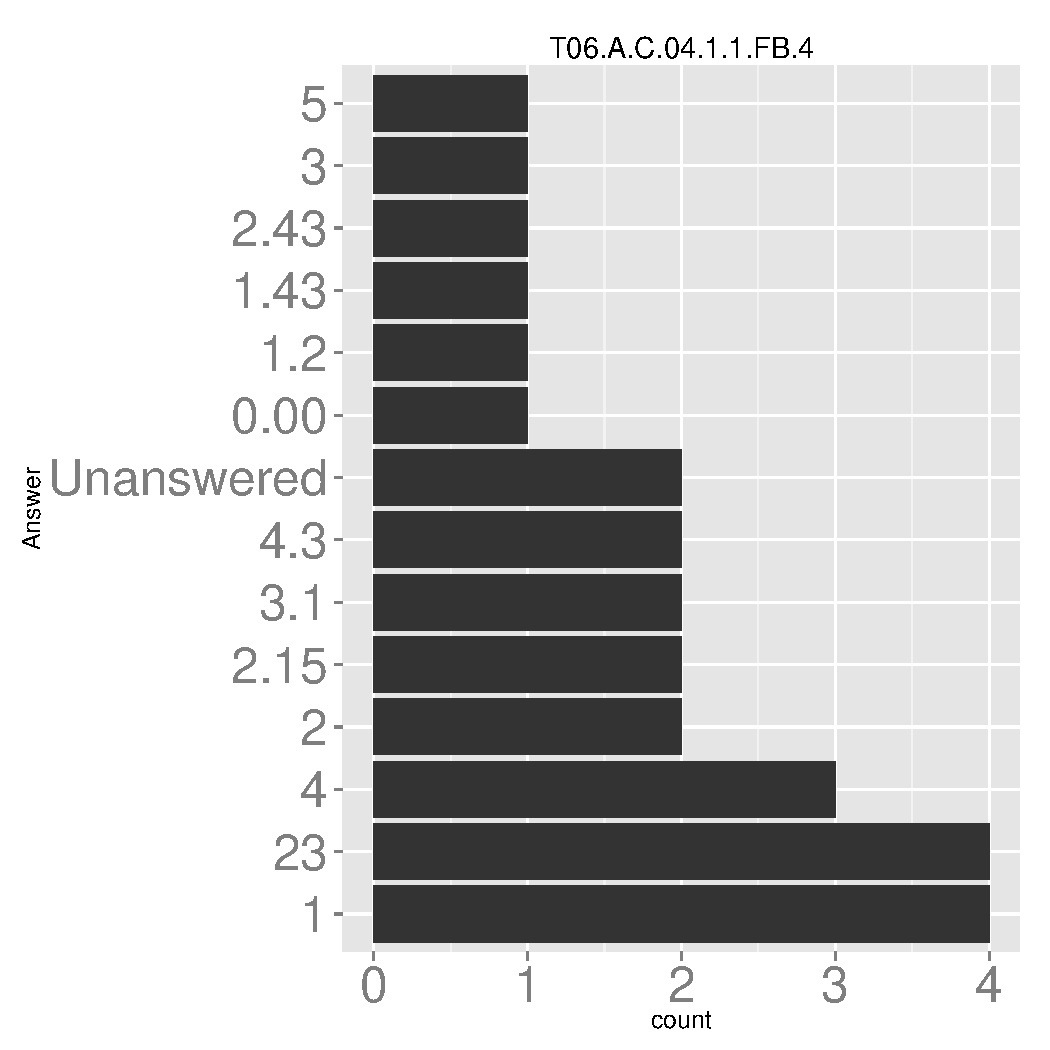
\includegraphics[width=.45\linewidth]{Topic06_12_answer} 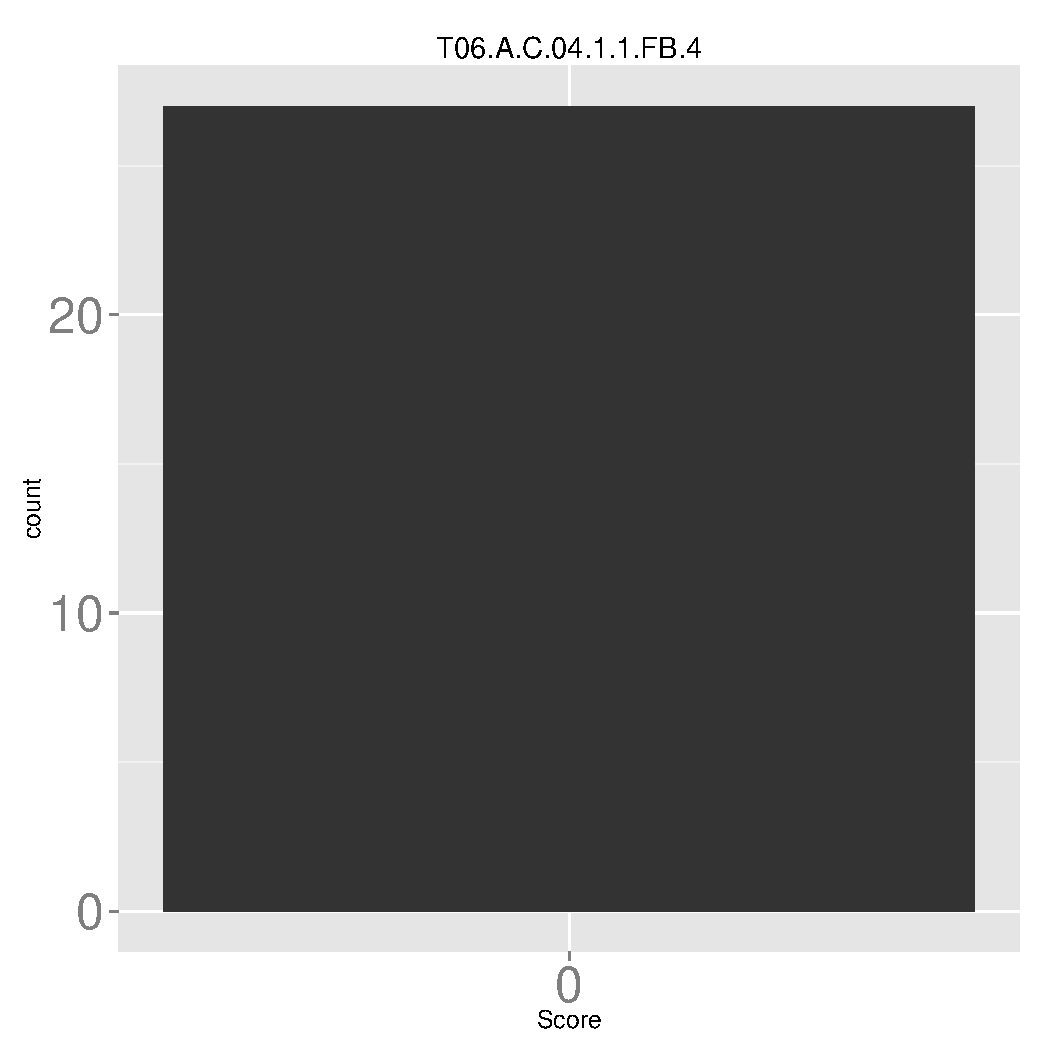
\includegraphics[width=.45\linewidth]{Topic06_12_score} \end{center} 

\begin{center}% latex table generated in R 3.2.2 by xtable 1.8-0 package
% Mon Nov 23 01:15:53 2015
\begin{tabular}{lr}
  \hline
Answer & Count \\ 
  \hline
1 &   4 \\ 
  23 &   4 \\ 
  4 &   3 \\ 
  2 &   2 \\ 
  2.15 &   2 \\ 
  3.1 &   2 \\ 
  4.3 &   2 \\ 
  Unanswered &   2 \\ 
  0.00 &   1 \\ 
  1.2 &   1 \\ 
  1.43 &   1 \\ 
  2.43 &   1 \\ 
  3 &   1 \\ 
  5 &   1 \\ 
   \hline
\end{tabular}
~~~~~~~~% latex table generated in R 3.2.2 by xtable 1.8-0 package
% Mon Nov 23 01:15:53 2015
\begin{tabular}{lr}
  \hline
Summary & Value \\ 
  \hline
Mean & 0.00 \\ 
  Std.dev & 0.00 \\ 
  Min & 0.00 \\ 
  Median & 0.00 \\ 
  Max & 0.00 \\ 
   \hline
\end{tabular}
\end{center}\newpage\marginnote{

 In a sample of 25 male newborns, the mean birth weight was 3.4 kg and the standard deviation was 0.35 kg.



The z-score for a birth weight of 2.3 kg is \_\_\_\_\_\_\_\_\_\_. Round your answer to 2 decimal places.



Correct Answer(s):



a. -3.14



b. -3.13



c. -3.15 

}\pdfbookmark[2]{T06.A.D.04.1.1.FB.1}{T06.A.D.04.1.1.FB.1} (13) Question "T06.A.D.04.1.1.FB.1" is given on the right. This question was selected from the question set with a frequency of 0.25. The question was administered to 20 out of the total of 100 students. The average score was 0 out of 1.

 (Back to the question summary Table \ref{tab:summary_question}.)

\begin{center} 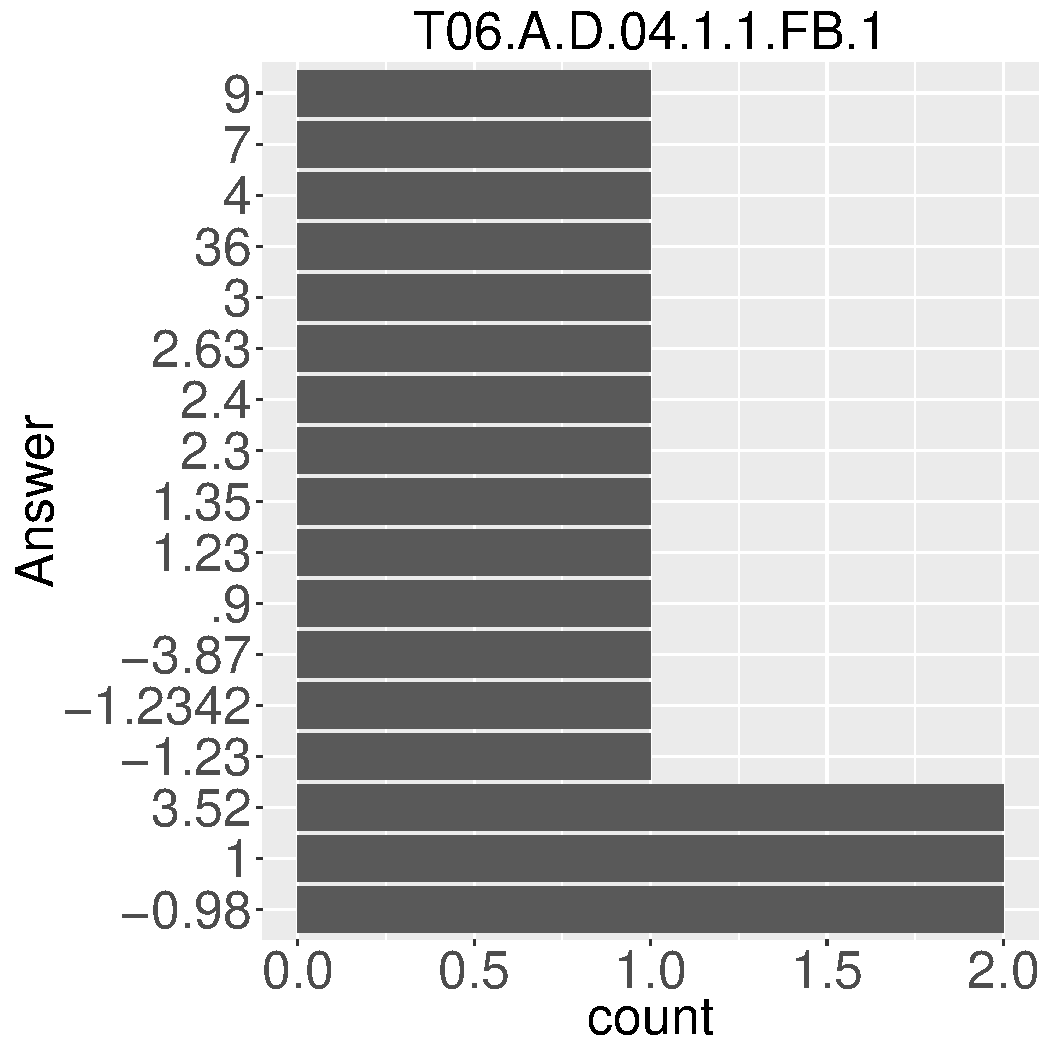
\includegraphics[width=.45\linewidth]{Topic06_13_answer} 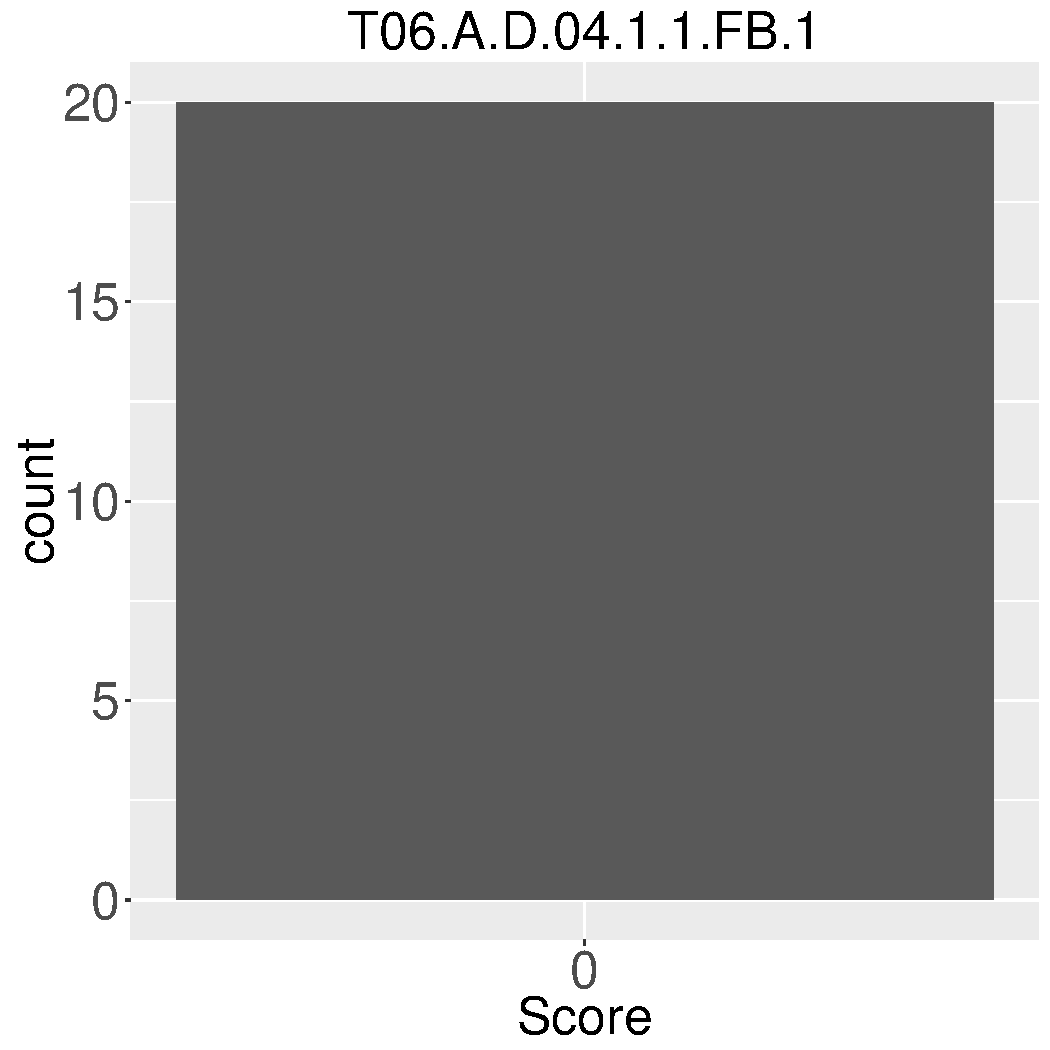
\includegraphics[width=.45\linewidth]{Topic06_13_score} \end{center} 

\begin{center}% latex table generated in R 3.2.2 by xtable 1.8-0 package
% Mon Nov 23 01:15:53 2015
\begin{tabular}{lr}
  \hline
Answer & Count \\ 
  \hline
-0.98 &   2 \\ 
  1 &   2 \\ 
  3.52 &   2 \\ 
  -1.23 &   1 \\ 
  -1.2342 &   1 \\ 
  -3.87 &   1 \\ 
  .9 &   1 \\ 
  1.23 &   1 \\ 
  1.35 &   1 \\ 
  2.3 &   1 \\ 
  2.4 &   1 \\ 
  2.63 &   1 \\ 
  3 &   1 \\ 
  36 &   1 \\ 
  4 &   1 \\ 
  7 &   1 \\ 
  9 &   1 \\ 
   \hline
\end{tabular}
~~~~~~~~% latex table generated in R 3.2.2 by xtable 1.8-0 package
% Mon Nov 23 01:15:53 2015
\begin{tabular}{lr}
  \hline
Summary & Value \\ 
  \hline
Mean & 0.00 \\ 
  Std.dev & 0.00 \\ 
  Min & 0.00 \\ 
  Median & 0.00 \\ 
  Max & 0.00 \\ 
   \hline
\end{tabular}
\end{center}\newpage\marginnote{

 In a sample of 25 male newborns, the mean birth weight was 3.4 kg and the standard deviation was 0.35 kg.



The z-score for a birth weight of 2.5 kg is \_\_\_\_\_\_\_\_\_\_. Round your answer to 2 decimal places.



Correct Answer(s):



a. -2.57



b. -2.58



c. -2.56 

}\pdfbookmark[2]{T06.A.D.04.1.1.FB.2}{T06.A.D.04.1.1.FB.2} (14) Question "T06.A.D.04.1.1.FB.2" is given on the right. This question was selected from the question set with a frequency of 0.25. The question was administered to 27 out of the total of 100 students. The average score was 0 out of 1.

 (Back to the question summary Table \ref{tab:summary_question}.)

\begin{center} 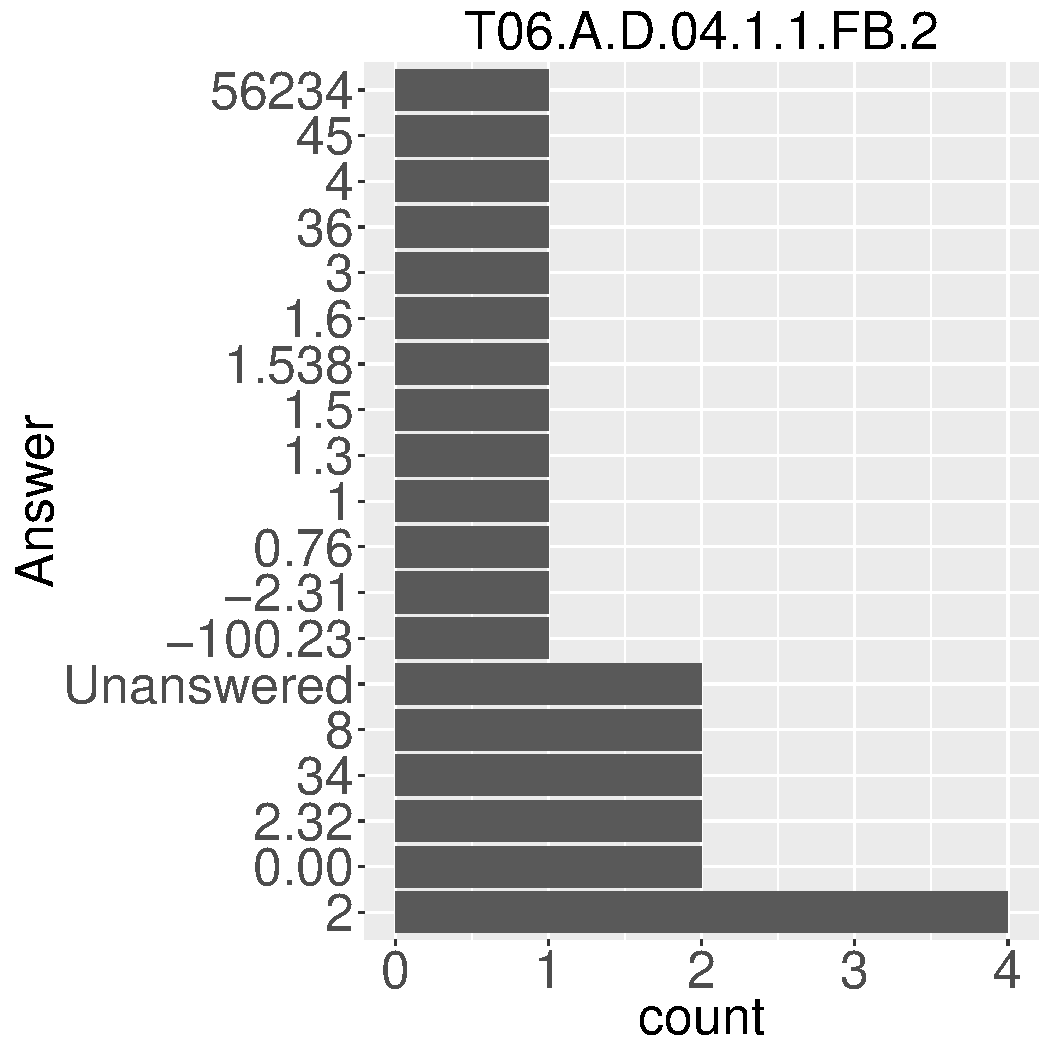
\includegraphics[width=.45\linewidth]{Topic06_14_answer} 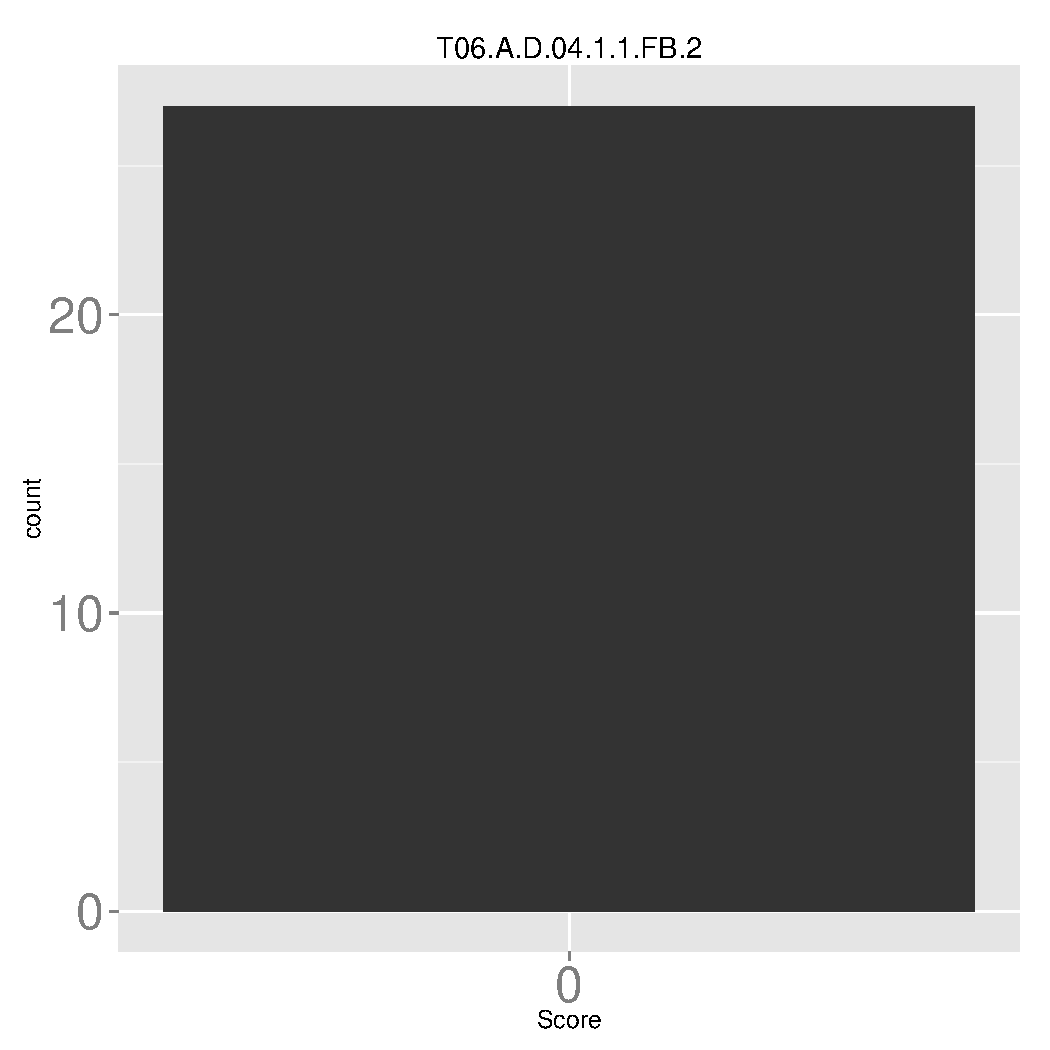
\includegraphics[width=.45\linewidth]{Topic06_14_score} \end{center} 

\begin{center}% latex table generated in R 3.2.2 by xtable 1.8-0 package
% Mon Nov 23 01:15:54 2015
\begin{tabular}{lr}
  \hline
Answer & Count \\ 
  \hline
2 &   4 \\ 
  0.00 &   2 \\ 
  2.32 &   2 \\ 
  34 &   2 \\ 
  8 &   2 \\ 
  Unanswered &   2 \\ 
  -100.23 &   1 \\ 
  -2.31 &   1 \\ 
  0.76 &   1 \\ 
  1 &   1 \\ 
  1.3 &   1 \\ 
  1.5 &   1 \\ 
  1.538 &   1 \\ 
  1.6 &   1 \\ 
  3 &   1 \\ 
  36 &   1 \\ 
  4 &   1 \\ 
  45 &   1 \\ 
  56234 &   1 \\ 
   \hline
\end{tabular}
~~~~~~~~% latex table generated in R 3.2.2 by xtable 1.8-0 package
% Mon Nov 23 01:15:54 2015
\begin{tabular}{lr}
  \hline
Summary & Value \\ 
  \hline
Mean & 0.00 \\ 
  Std.dev & 0.00 \\ 
  Min & 0.00 \\ 
  Median & 0.00 \\ 
  Max & 0.00 \\ 
   \hline
\end{tabular}
\end{center}\newpage\marginnote{

 In a sample of 25 male newborns, the mean birth weight was 3.4 kg and the standard deviation was 0.35 kg.



The z-score for a birth weight of 2.2 kg is \_\_\_\_\_\_\_\_\_\_. Round your answer to 2 decimal places.



Correct Answer(s):



a. -3.43



b. -3.44



c. -3.42 

}\pdfbookmark[2]{T06.A.D.04.1.1.FB.3}{T06.A.D.04.1.1.FB.3} (15) Question "T06.A.D.04.1.1.FB.3" is given on the right. This question was selected from the question set with a frequency of 0.25. The question was administered to 24 out of the total of 100 students. The average score was 0 out of 1.

 (Back to the question summary Table \ref{tab:summary_question}.)

\begin{center} 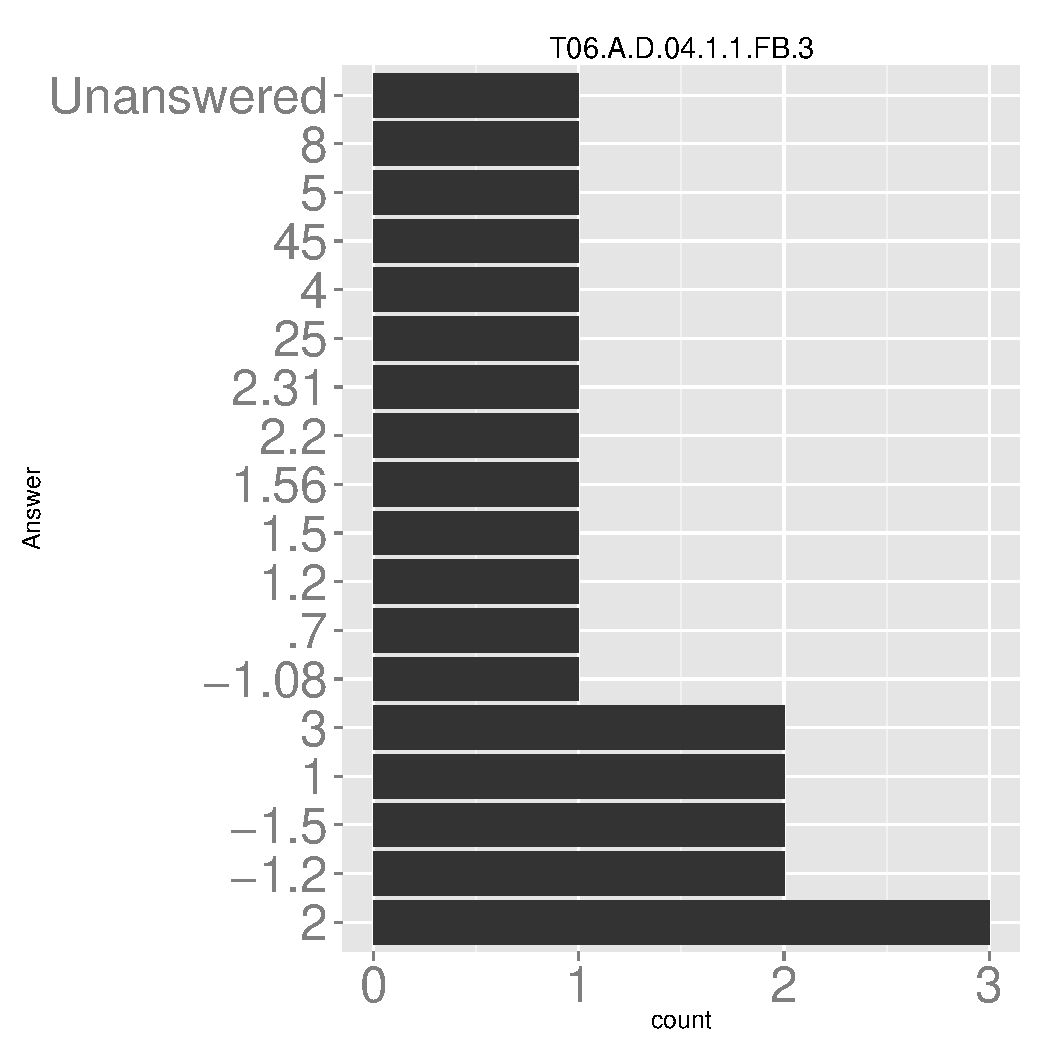
\includegraphics[width=.45\linewidth]{Topic06_15_answer} 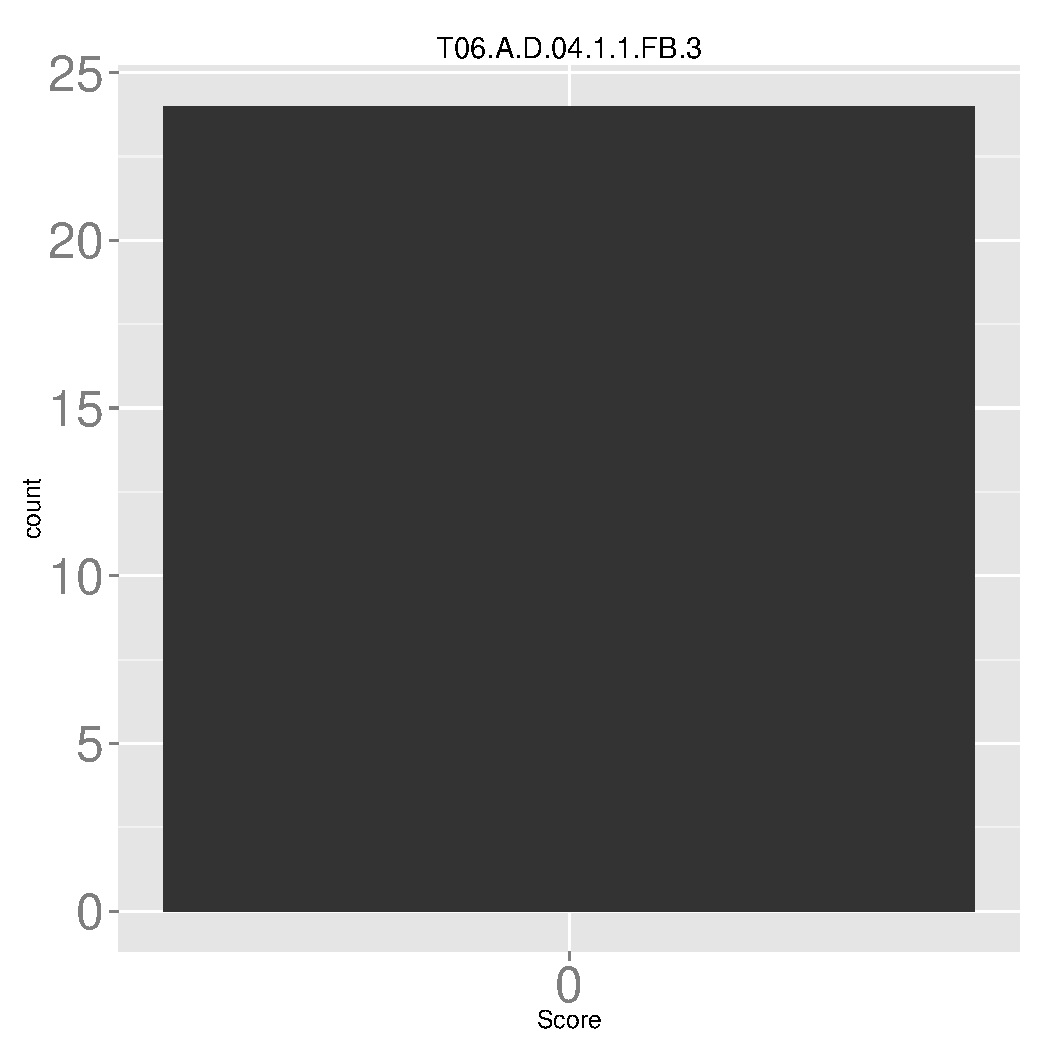
\includegraphics[width=.45\linewidth]{Topic06_15_score} \end{center} 

\begin{center}% latex table generated in R 3.2.2 by xtable 1.8-0 package
% Mon Nov 23 01:15:54 2015
\begin{tabular}{lr}
  \hline
Answer & Count \\ 
  \hline
2 &   3 \\ 
  -1.2 &   2 \\ 
  -1.5 &   2 \\ 
  1 &   2 \\ 
  3 &   2 \\ 
  -1.08 &   1 \\ 
  .7 &   1 \\ 
  1.2 &   1 \\ 
  1.5 &   1 \\ 
  1.56 &   1 \\ 
  2.2 &   1 \\ 
  2.31 &   1 \\ 
  25 &   1 \\ 
  4 &   1 \\ 
  45 &   1 \\ 
  5 &   1 \\ 
  8 &   1 \\ 
  Unanswered &   1 \\ 
   \hline
\end{tabular}
~~~~~~~~% latex table generated in R 3.2.2 by xtable 1.8-0 package
% Mon Nov 23 01:15:54 2015
\begin{tabular}{lr}
  \hline
Summary & Value \\ 
  \hline
Mean & 0.00 \\ 
  Std.dev & 0.00 \\ 
  Min & 0.00 \\ 
  Median & 0.00 \\ 
  Max & 0.00 \\ 
   \hline
\end{tabular}
\end{center}\newpage\marginnote{

 In a sample of 25 male newborns, the mean birth weight was 3.4 kg and the standard deviation was 0.35 kg.



The z-score for a birth weight of 2.8 kg is \_\_\_\_\_\_\_\_\_\_. Round your answer to 2 decimal places.



Correct Answer(s):



a. -1.71



b. -1.72



c. -1.70



d. -1.7 

}\pdfbookmark[2]{T06.A.D.04.1.1.FB.4}{T06.A.D.04.1.1.FB.4} (16) Question "T06.A.D.04.1.1.FB.4" is given on the right. This question was selected from the question set with a frequency of 0.25. The question was administered to 29 out of the total of 100 students. The average score was 0 out of 1.

 (Back to the question summary Table \ref{tab:summary_question}.)

\begin{center} 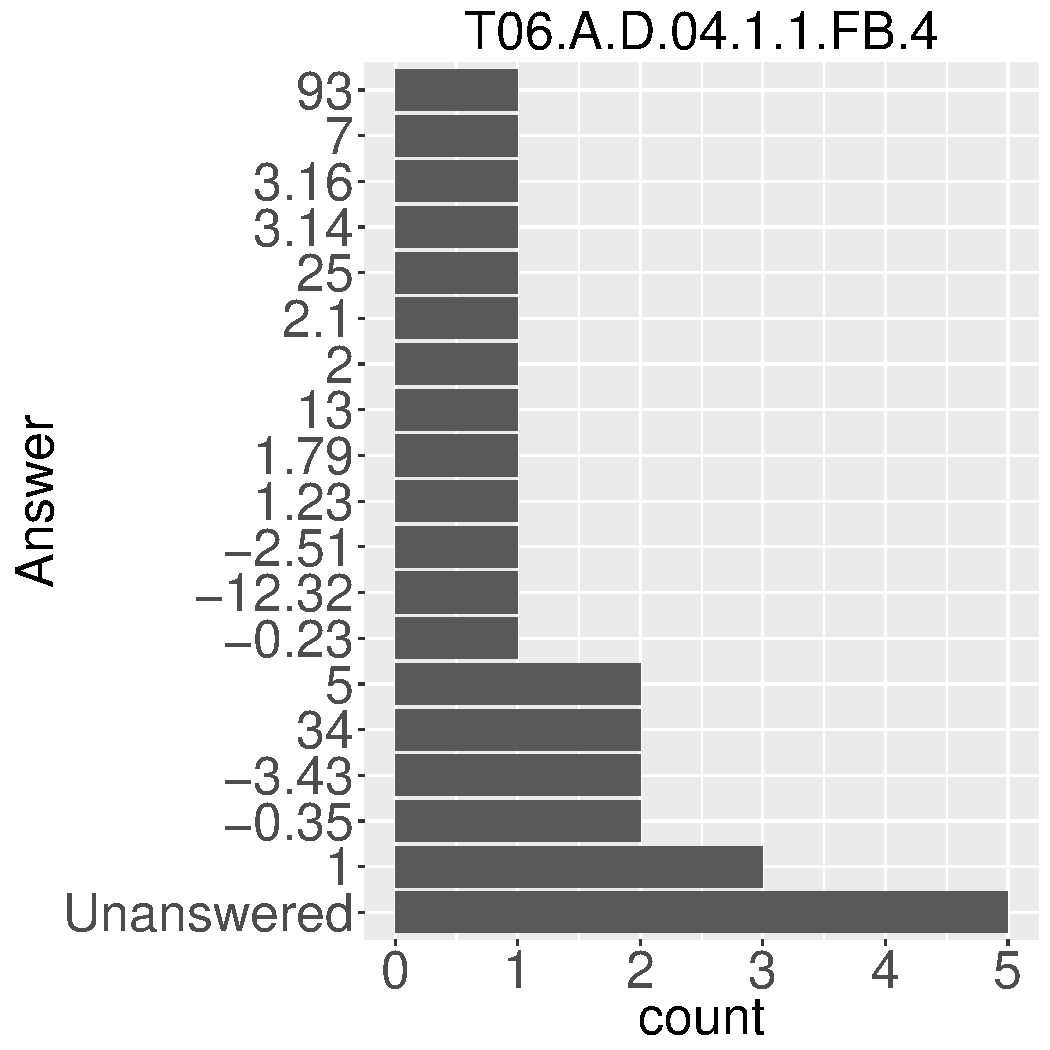
\includegraphics[width=.45\linewidth]{Topic06_16_answer} 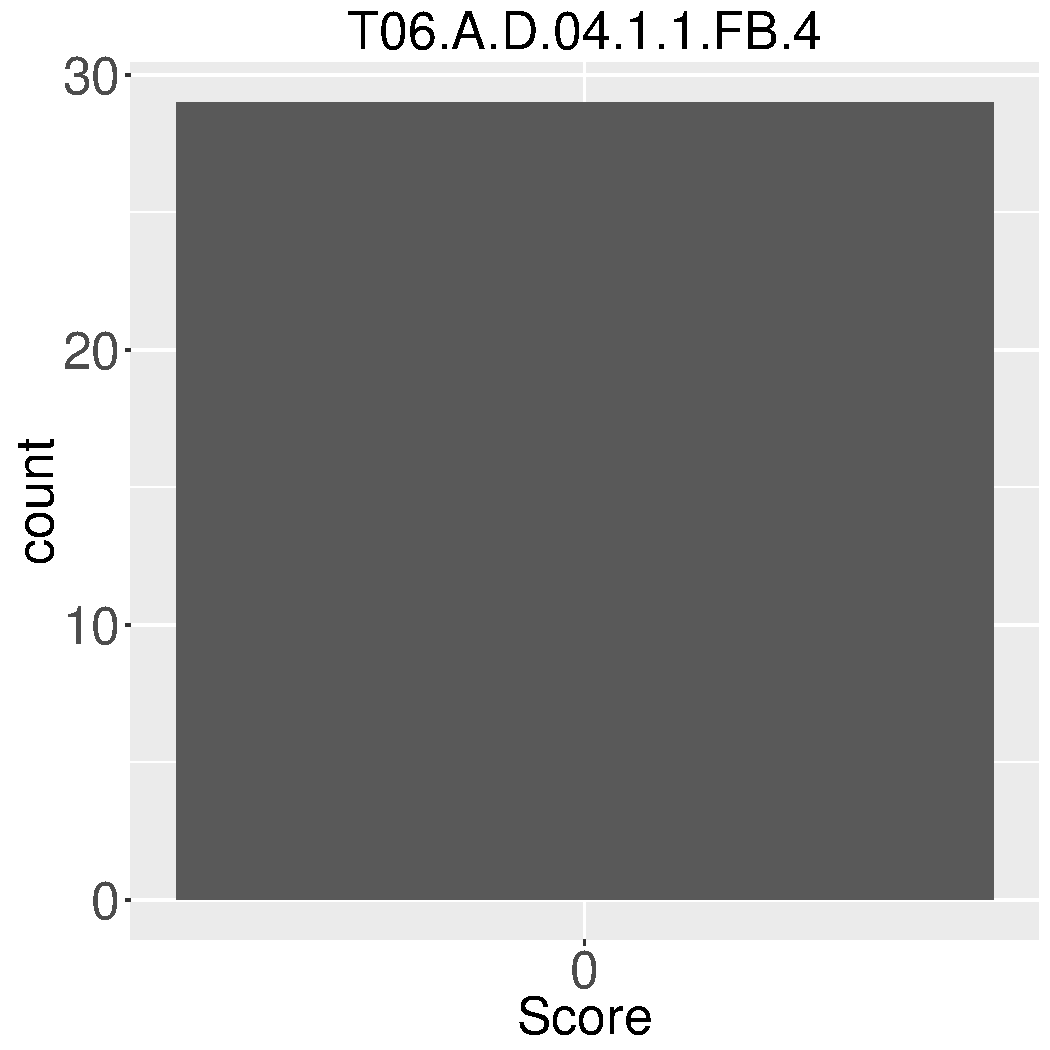
\includegraphics[width=.45\linewidth]{Topic06_16_score} \end{center} 

\begin{center}% latex table generated in R 3.2.2 by xtable 1.8-0 package
% Mon Nov 23 01:15:54 2015
\begin{tabular}{lr}
  \hline
Answer & Count \\ 
  \hline
Unanswered &   5 \\ 
  1 &   3 \\ 
  -0.35 &   2 \\ 
  -3.43 &   2 \\ 
  34 &   2 \\ 
  5 &   2 \\ 
  -0.23 &   1 \\ 
  -12.32 &   1 \\ 
  -2.51 &   1 \\ 
  1.23 &   1 \\ 
  1.79 &   1 \\ 
  13 &   1 \\ 
  2 &   1 \\ 
  2.1 &   1 \\ 
  25 &   1 \\ 
  3.14 &   1 \\ 
  3.16 &   1 \\ 
  7 &   1 \\ 
  93 &   1 \\ 
   \hline
\end{tabular}
~~~~~~~~% latex table generated in R 3.2.2 by xtable 1.8-0 package
% Mon Nov 23 01:15:55 2015
\begin{tabular}{lr}
  \hline
Summary & Value \\ 
  \hline
Mean & 0.00 \\ 
  Std.dev & 0.00 \\ 
  Min & 0.00 \\ 
  Median & 0.00 \\ 
  Max & 0.00 \\ 
   \hline
\end{tabular}
\end{center}\newpage\marginnote{

 The height of adult women is thought to have a mean of 65 inches and a standard deviation of 2.5 inches. The height of adult men is thought to have a mean of 71 inches and a standard deviation of 3 inches. In the same family, the son is 73 inches tall and the daughter is 67 inches tall. Who is taller among their gender, the son or daughter?



*a. The daughter



b. The son



c. The daughter and son are the same height within their gender. 

}\pdfbookmark[2]{T06.B.E.01.1.1.MC.compare1}{T06.B.E.01.1.1.MC.compare1} (17) Question "T06.B.E.01.1.1.MC.compare1" is given on the right. This question was selected from the question set with a frequency of 1. The question was administered to 100 out of the total of 100 students. The average score was 0.41 out of 1.

 (Back to the question summary Table \ref{tab:summary_question}.)

\begin{center} 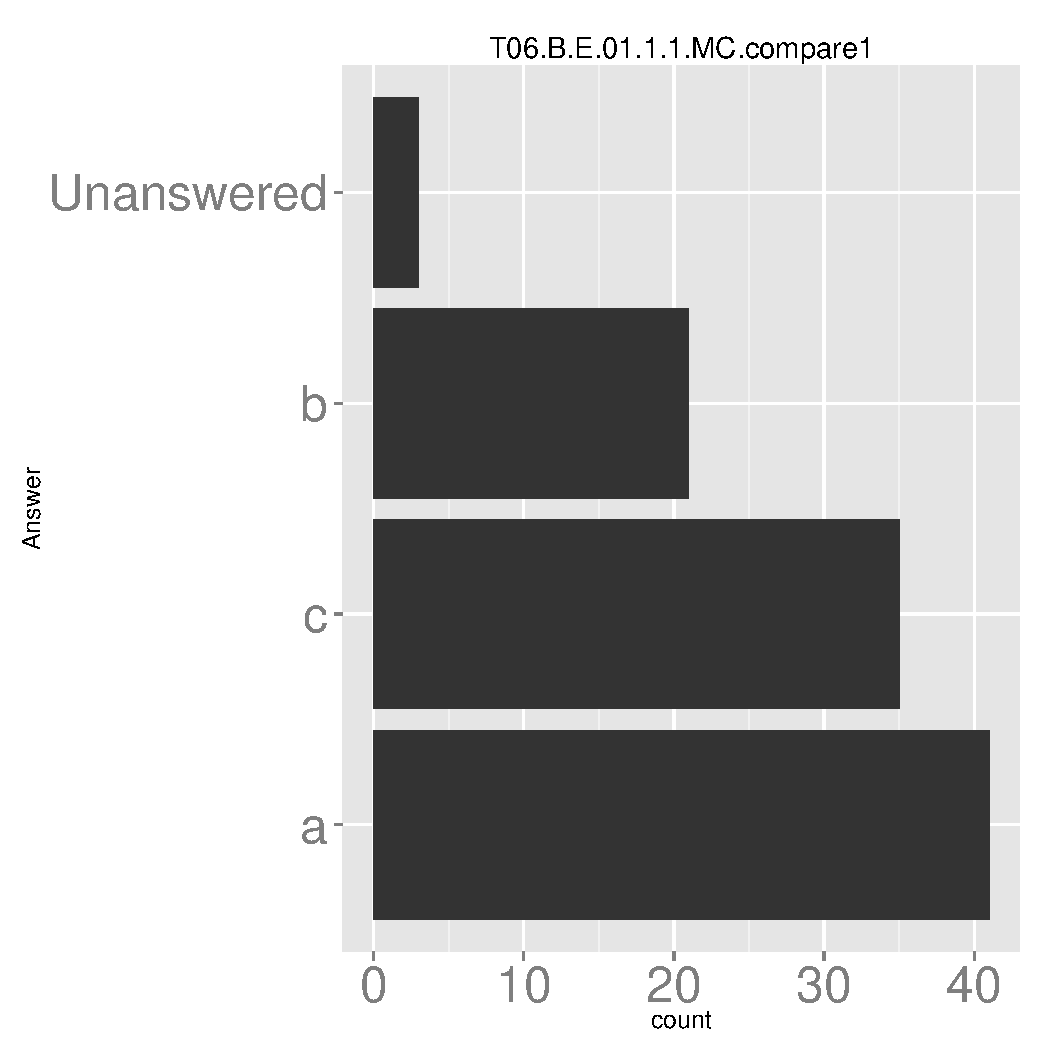
\includegraphics[width=.45\linewidth]{Topic06_17_answer} 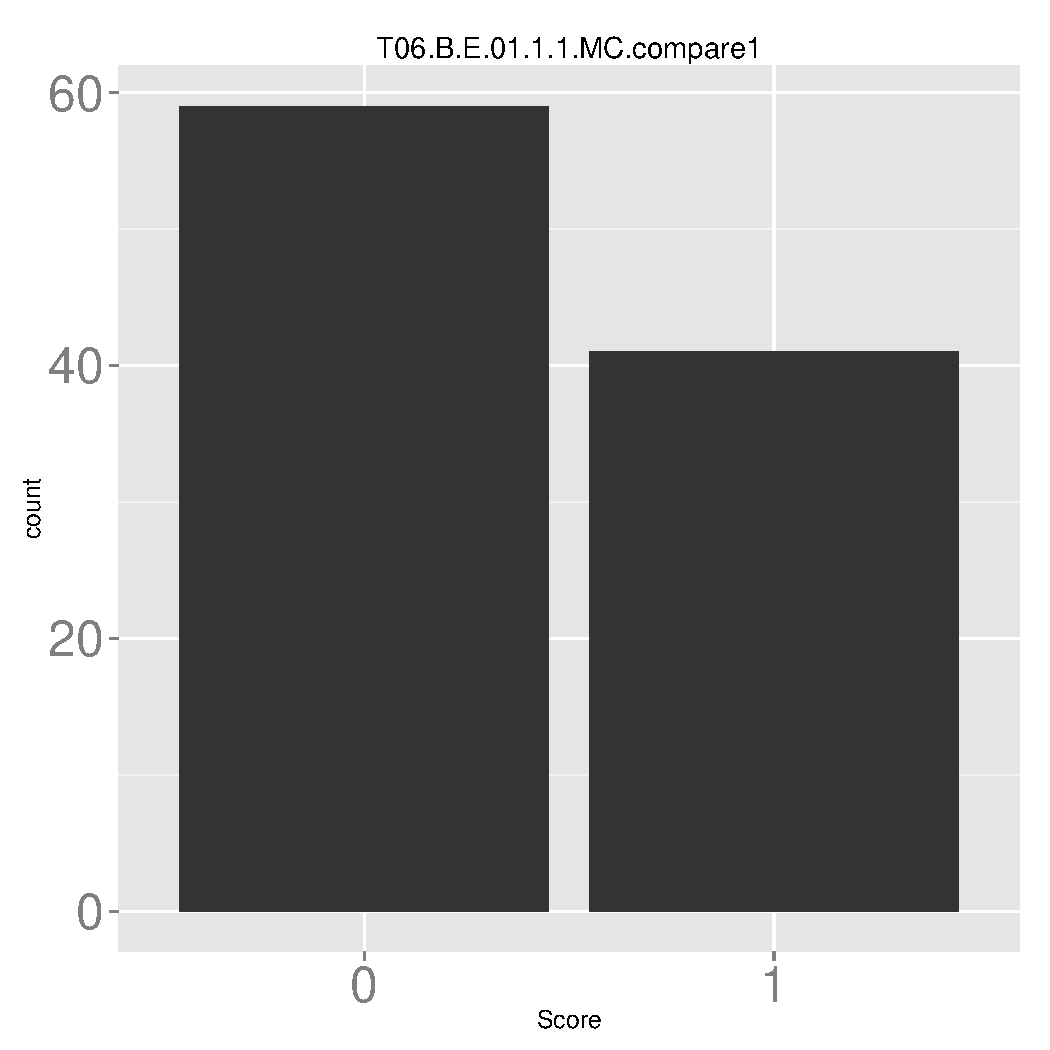
\includegraphics[width=.45\linewidth]{Topic06_17_score} \end{center} 

\begin{center}% latex table generated in R 3.2.2 by xtable 1.8-0 package
% Mon Nov 23 01:15:55 2015
\begin{tabular}{lr}
  \hline
Answer & Count \\ 
  \hline
a &  41 \\ 
  c &  35 \\ 
  b &  21 \\ 
  Unanswered &   3 \\ 
   \hline
\end{tabular}
~~~~~~~~% latex table generated in R 3.2.2 by xtable 1.8-0 package
% Mon Nov 23 01:15:55 2015
\begin{tabular}{lr}
  \hline
Summary & Value \\ 
  \hline
Mean & 0.41 \\ 
  Std.dev & 0.49 \\ 
  Min & 0.00 \\ 
  Median & 0.00 \\ 
  Max & 1.00 \\ 
   \hline
\end{tabular}
\end{center}\newpage\marginnote{

 The height of adult women is thought to have a mean of 65 inches and a standard deviation of 2.5 inches. The height of adult men is thought to have a mean of 71 inches and a standard deviation of 3 inches. In the same family, the son is 67 inches tall and the daughter is 59 inches tall. Who is taller among their gender, the son or daughter?



a. The daughter



*b. The son



c. The daughter and son are the same height within their gender. 

}\pdfbookmark[2]{T06.B.F.01.1.1.MC.compare2}{T06.B.F.01.1.1.MC.compare2} (18) Question "T06.B.F.01.1.1.MC.compare2" is given on the right. This question was selected from the question set with a frequency of 1. The question was administered to 100 out of the total of 100 students. The average score was 0.28 out of 1.

 (Back to the question summary Table \ref{tab:summary_question}.)

\begin{center} 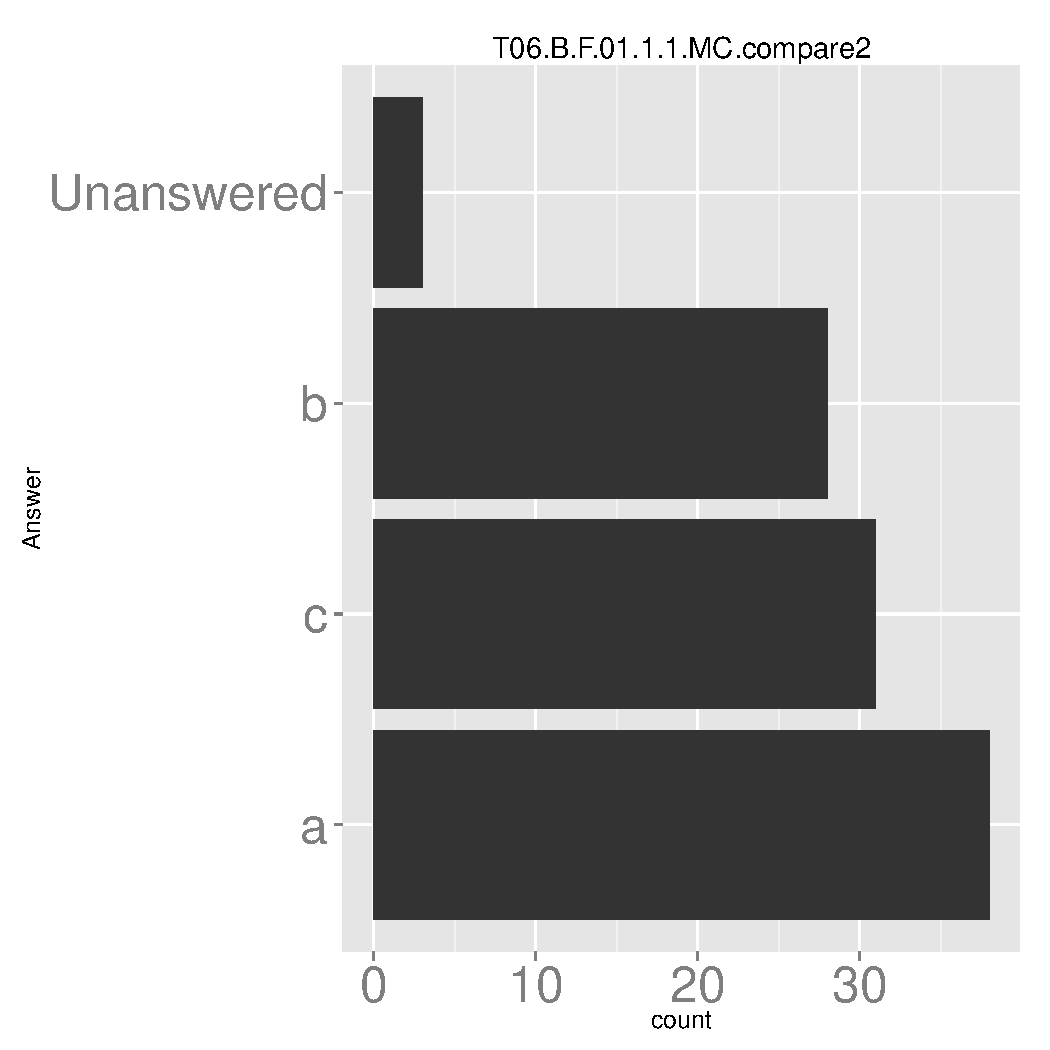
\includegraphics[width=.45\linewidth]{Topic06_18_answer} 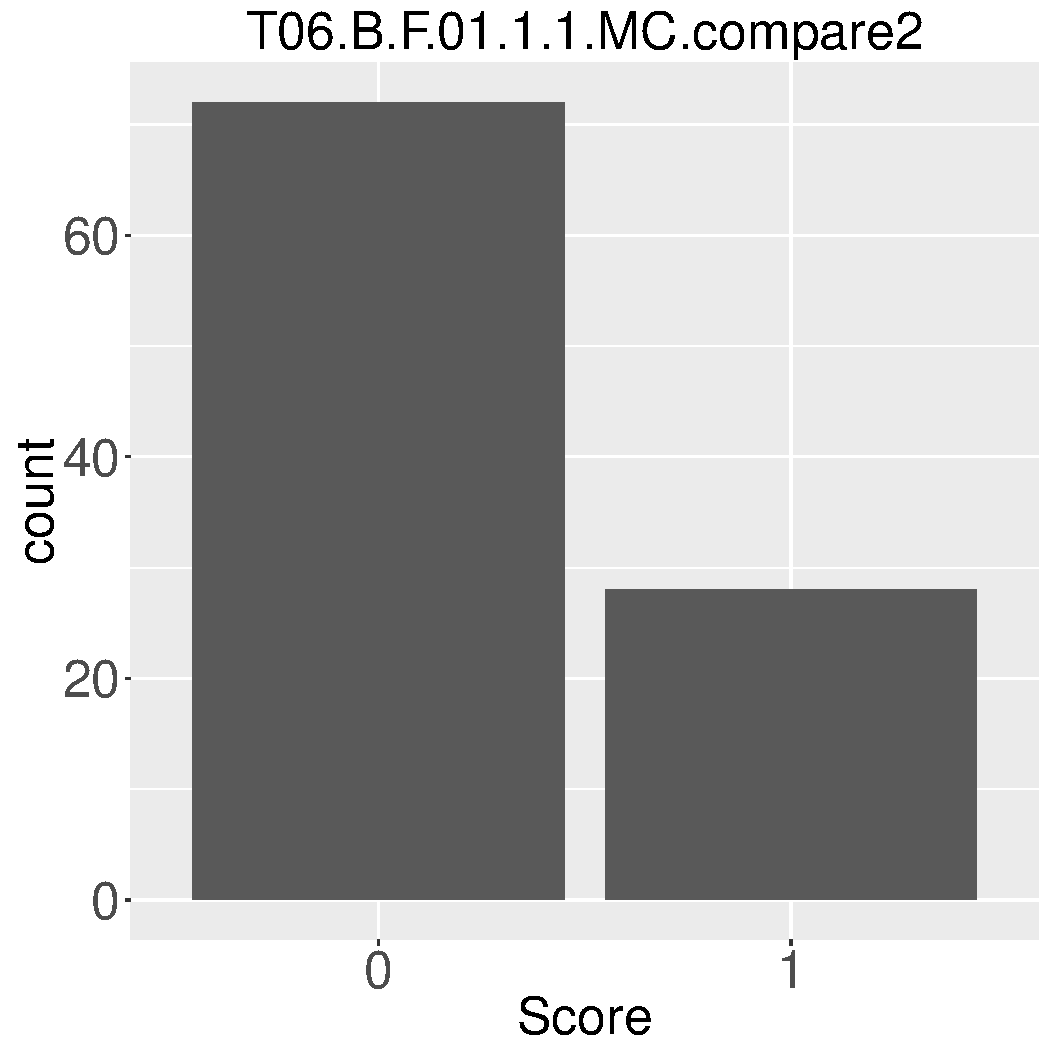
\includegraphics[width=.45\linewidth]{Topic06_18_score} \end{center} 

\begin{center}% latex table generated in R 3.2.2 by xtable 1.8-0 package
% Mon Nov 23 01:15:55 2015
\begin{tabular}{lr}
  \hline
Answer & Count \\ 
  \hline
a &  38 \\ 
  c &  31 \\ 
  b &  28 \\ 
  Unanswered &   3 \\ 
   \hline
\end{tabular}
~~~~~~~~% latex table generated in R 3.2.2 by xtable 1.8-0 package
% Mon Nov 23 01:15:55 2015
\begin{tabular}{lr}
  \hline
Summary & Value \\ 
  \hline
Mean & 0.28 \\ 
  Std.dev & 0.45 \\ 
  Min & 0.00 \\ 
  Median & 0.00 \\ 
  Max & 1.00 \\ 
   \hline
\end{tabular}
\end{center}\newpage\marginnote{

 Standardizing makes the following change(s) to a distribution: I. Shifts the distribution by subtracting the mean. II. Rescales the distribution by dividing by the standard deviation. III. Changes the skewness or symmetry of the distribution. IV. Creates outliers.



a. I, II, and III



*b. I and II



c. III and IV



d. II and III



e. I, II and IV 

}\pdfbookmark[2]{T06.C.G.01.1.1.MC.1}{T06.C.G.01.1.1.MC.1} (19) Question "T06.C.G.01.1.1.MC.1" is given on the right. This question was selected from the question set with a frequency of 1. The question was administered to 100 out of the total of 100 students. The average score was 0.2 out of 1.

 (Back to the question summary Table \ref{tab:summary_question}.)

\begin{center} 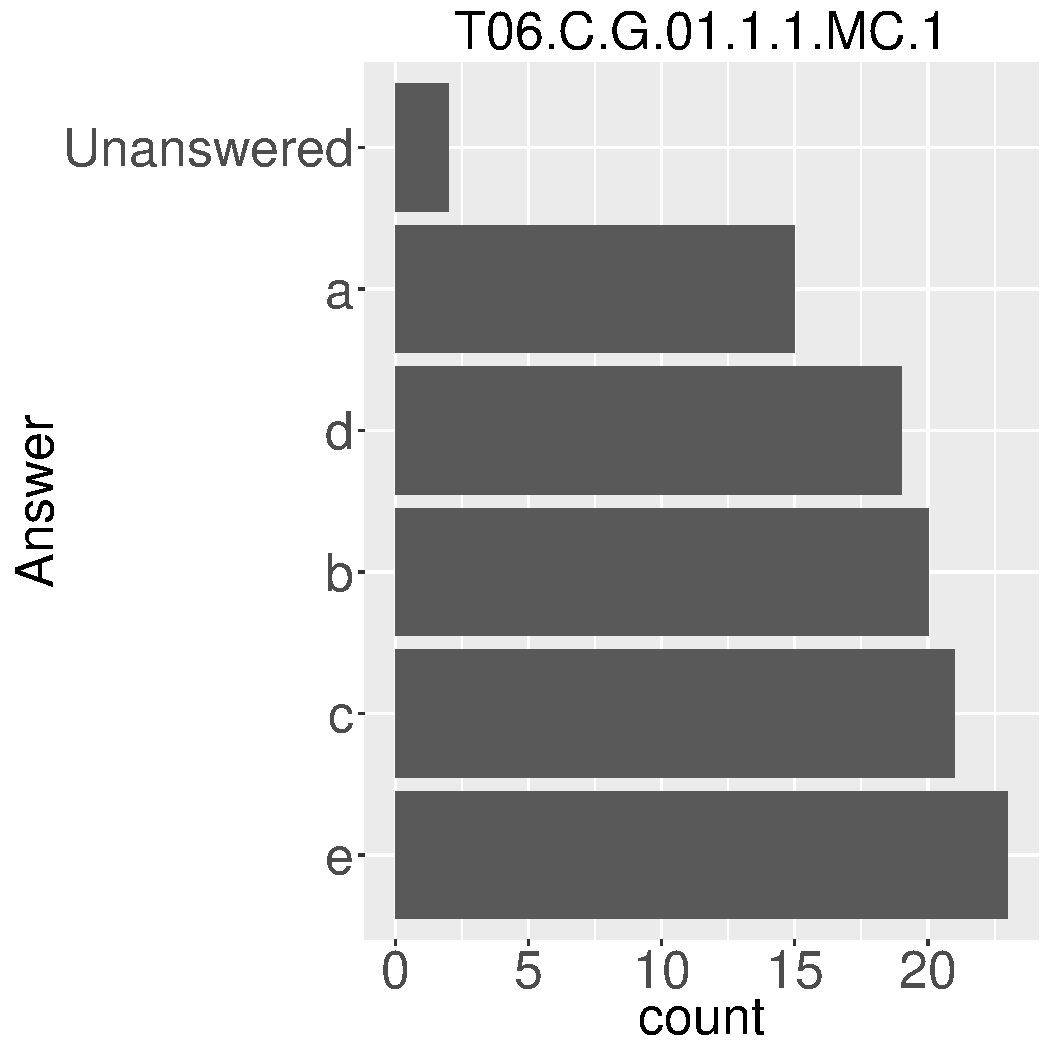
\includegraphics[width=.45\linewidth]{Topic06_19_answer} 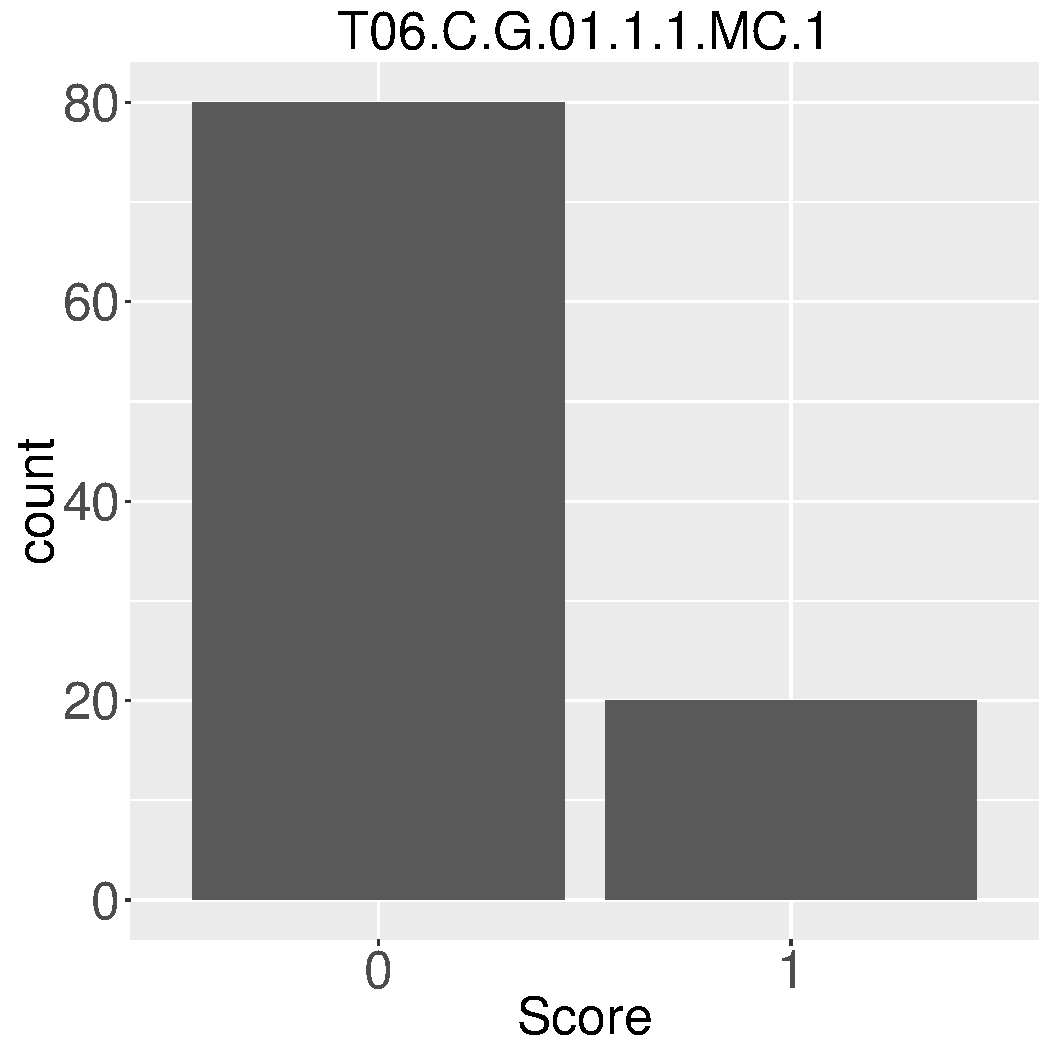
\includegraphics[width=.45\linewidth]{Topic06_19_score} \end{center} 

\begin{center}% latex table generated in R 3.2.2 by xtable 1.8-0 package
% Mon Nov 23 01:15:56 2015
\begin{tabular}{lr}
  \hline
Answer & Count \\ 
  \hline
e &  23 \\ 
  c &  21 \\ 
  b &  20 \\ 
  d &  19 \\ 
  a &  15 \\ 
  Unanswered &   2 \\ 
   \hline
\end{tabular}
~~~~~~~~% latex table generated in R 3.2.2 by xtable 1.8-0 package
% Mon Nov 23 01:15:56 2015
\begin{tabular}{lr}
  \hline
Summary & Value \\ 
  \hline
Mean & 0.20 \\ 
  Std.dev & 0.40 \\ 
  Min & 0.00 \\ 
  Median & 0.00 \\ 
  Max & 1.00 \\ 
   \hline
\end{tabular}
\end{center}\newpage\marginnote{

 Which part of the distribution is NOT affected by standardizing?



*a. shape



b. median



c. IQR



d. range 

}\pdfbookmark[2]{T06.C.H.01.1.1.MC.1}{T06.C.H.01.1.1.MC.1} (20) Question "T06.C.H.01.1.1.MC.1" is given on the right. This question was selected from the question set with a frequency of 1. The question was administered to 100 out of the total of 100 students. The average score was 0.24 out of 1.

 (Back to the question summary Table \ref{tab:summary_question}.)

\begin{center} 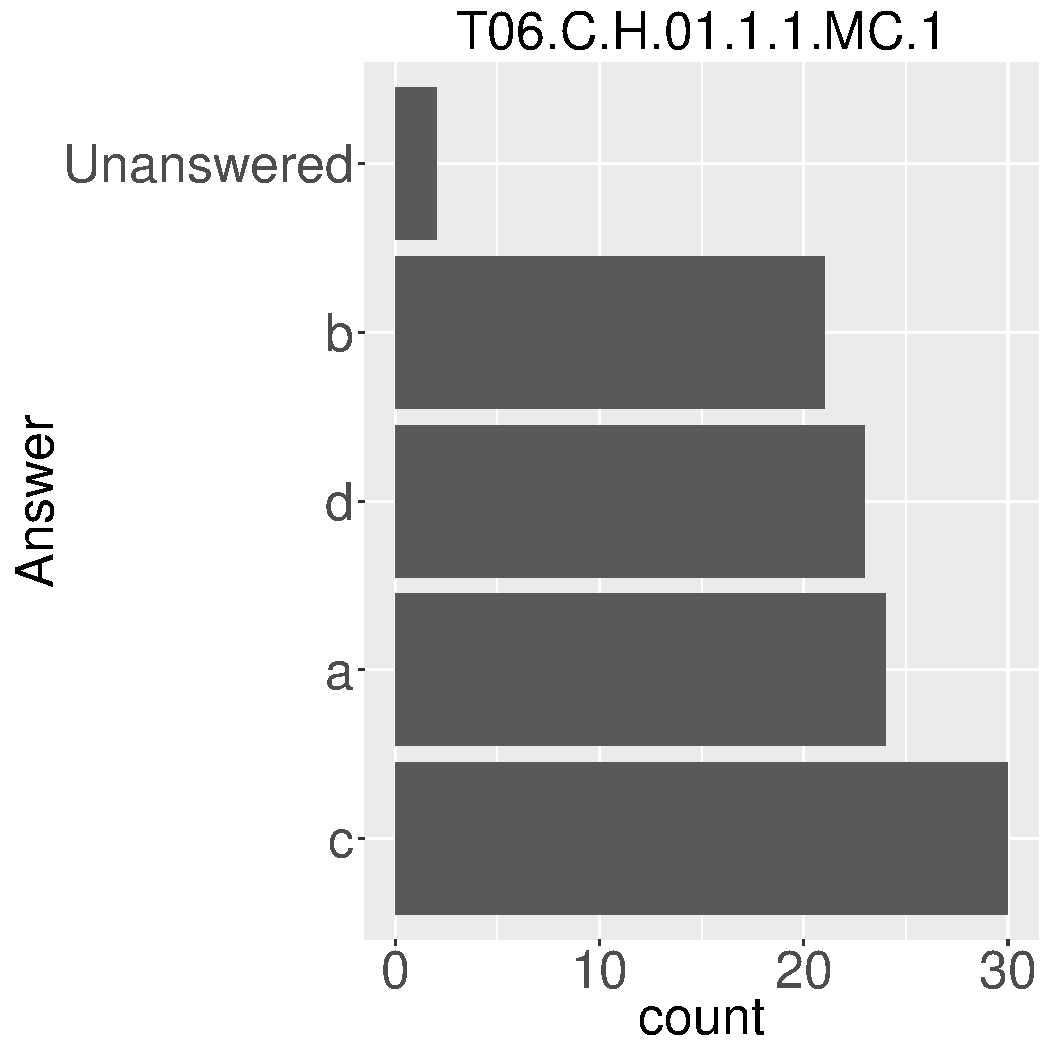
\includegraphics[width=.45\linewidth]{Topic06_20_answer} 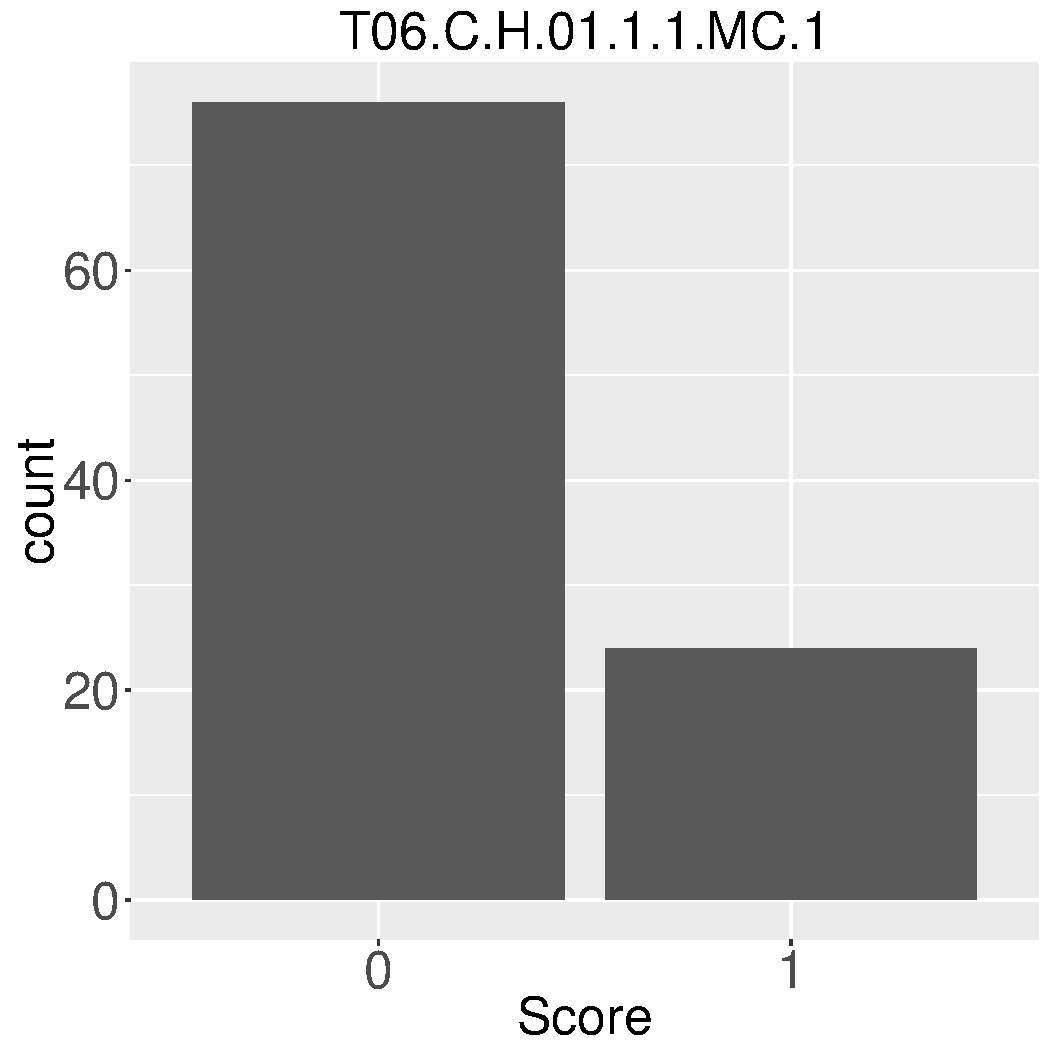
\includegraphics[width=.45\linewidth]{Topic06_20_score} \end{center} 

\begin{center}% latex table generated in R 3.2.2 by xtable 1.8-0 package
% Mon Nov 23 01:15:56 2015
\begin{tabular}{lr}
  \hline
Answer & Count \\ 
  \hline
c &  30 \\ 
  a &  24 \\ 
  d &  23 \\ 
  b &  21 \\ 
  Unanswered &   2 \\ 
   \hline
\end{tabular}
~~~~~~~~% latex table generated in R 3.2.2 by xtable 1.8-0 package
% Mon Nov 23 01:15:56 2015
\begin{tabular}{lr}
  \hline
Summary & Value \\ 
  \hline
Mean & 0.24 \\ 
  Std.dev & 0.43 \\ 
  Min & 0.00 \\ 
  Median & 0.00 \\ 
  Max & 1.00 \\ 
   \hline
\end{tabular}
\end{center}\newpage\marginnote{

 NBA players tend to have very large feet. The following plots display what these shoe sizes may hypothetically look like. Based on the output, it is reasonable to model the distribution of NBA players shoe sizes with a normal distribution. 

}



\vspace{5cm}\begin{marginfigure}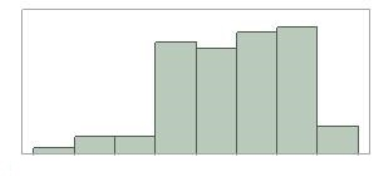
\includegraphics[width=0.98\linewidth]{/Users/lindz/ePort/inst/extdata/KeyFiles/Topic06.Questions_files/image002}\end{marginfigure}\marginnote{

 *a. True



b. False 

}\vspace{-5cm}\pdfbookmark[2]{T06.D.I.02.1.1.TF.feet}{T06.D.I.02.1.1.TF.feet} (21) Question "T06.D.I.02.1.1.TF.feet" is given on the right. This question was selected from the question set with a frequency of 0.5. The question was administered to 46 out of the total of 100 students. The average score was 0.74 out of 1.

 (Back to the question summary Table \ref{tab:summary_question}.)

\begin{center} 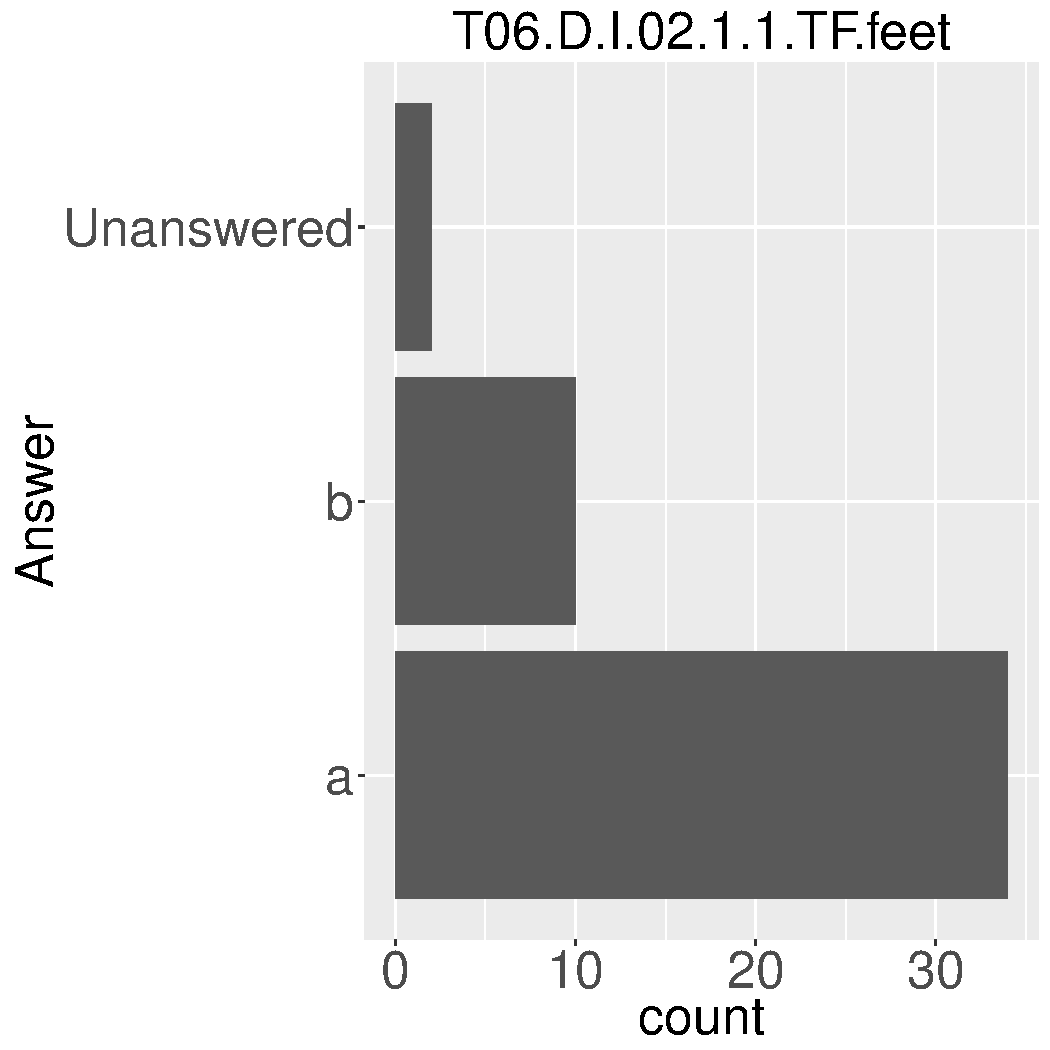
\includegraphics[width=.45\linewidth]{Topic06_21_answer} 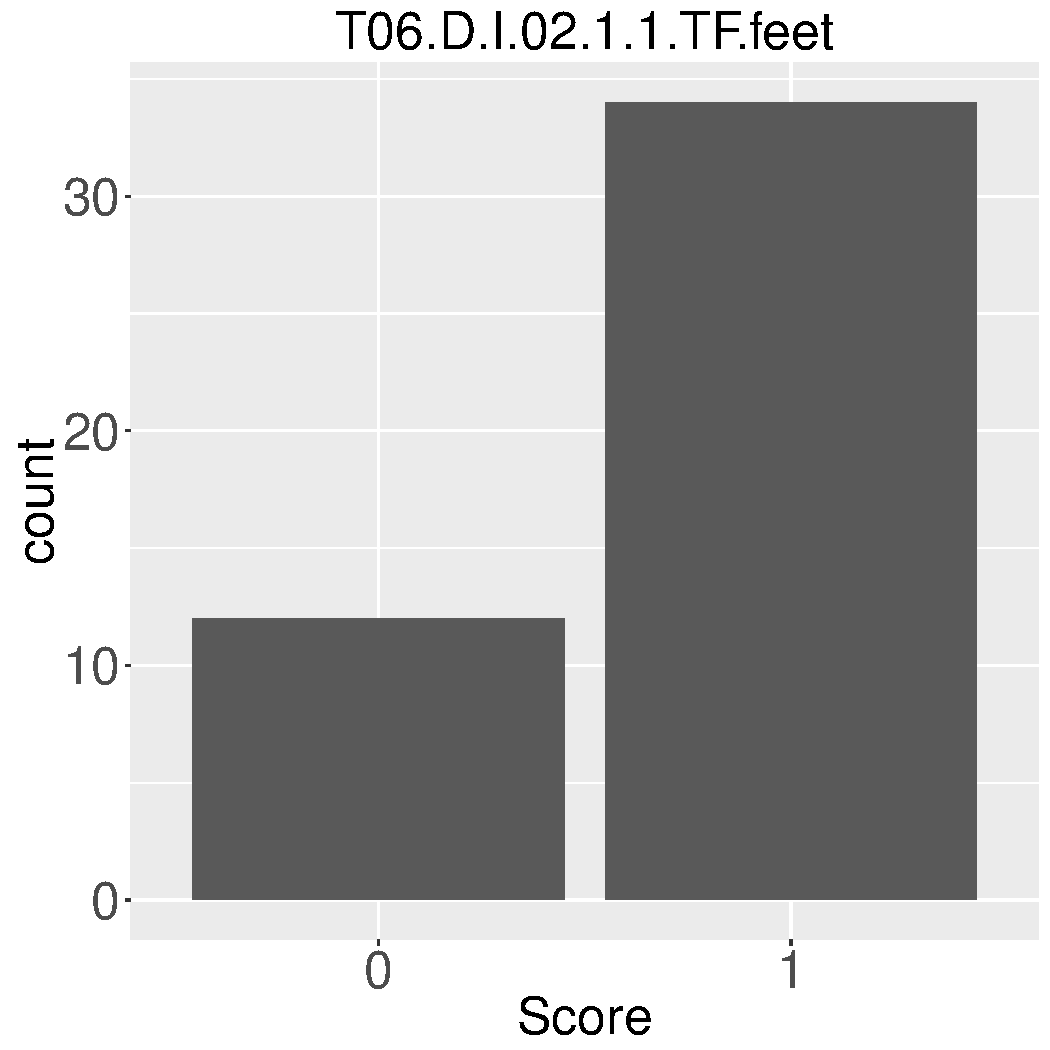
\includegraphics[width=.45\linewidth]{Topic06_21_score} \end{center} 

\begin{center}% latex table generated in R 3.2.2 by xtable 1.8-0 package
% Mon Nov 23 01:15:57 2015
\begin{tabular}{lr}
  \hline
Answer & Count \\ 
  \hline
a &  34 \\ 
  b &  10 \\ 
  Unanswered &   2 \\ 
   \hline
\end{tabular}
~~~~~~~~% latex table generated in R 3.2.2 by xtable 1.8-0 package
% Mon Nov 23 01:15:57 2015
\begin{tabular}{lr}
  \hline
Summary & Value \\ 
  \hline
Mean & 0.74 \\ 
  Std.dev & 0.44 \\ 
  Min & 0.00 \\ 
  Median & 1.00 \\ 
  Max & 1.00 \\ 
   \hline
\end{tabular}
\end{center}\newpage\marginnote{

 Below is the distribution of low temperatures (in degrees F) for 52 cities in the U.S. Based on the output, it is reasonable to model the distribution of low temperature for these cities with a normal distribution. 

}



\vspace{5cm}\begin{marginfigure}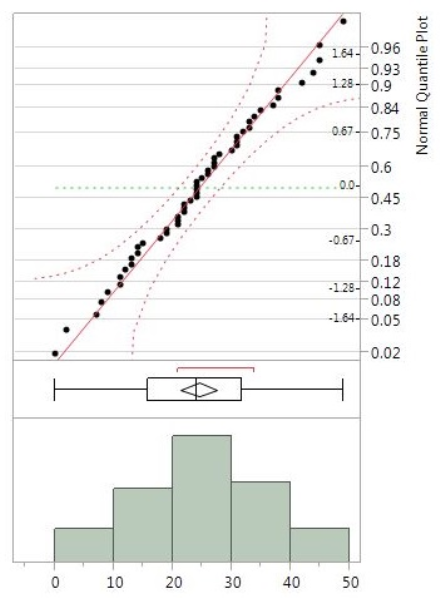
\includegraphics[width=0.98\linewidth]{/Users/lindz/ePort/inst/extdata/KeyFiles/Topic06.Questions_files/image004}\end{marginfigure}\marginnote{

 *a. True



b. False 

}\vspace{-5cm}\pdfbookmark[2]{T06.D.I.02.1.1.TF.lowtemp}{T06.D.I.02.1.1.TF.lowtemp} (22) Question "T06.D.I.02.1.1.TF.lowtemp" is given on the right. This question was selected from the question set with a frequency of 0.5. The question was administered to 54 out of the total of 100 students. The average score was 0.7 out of 1.

 (Back to the question summary Table \ref{tab:summary_question}.)

\begin{center} 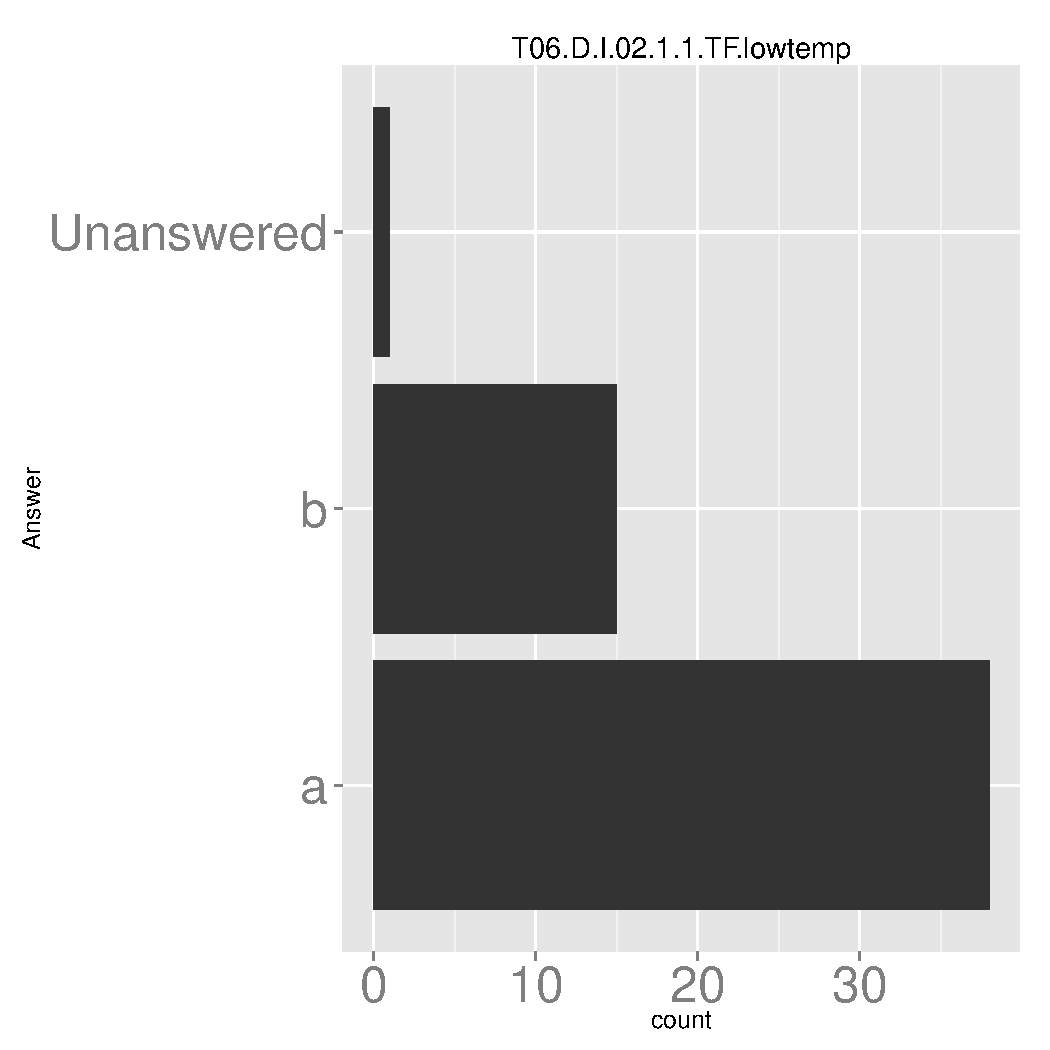
\includegraphics[width=.45\linewidth]{Topic06_22_answer} \includegraphics[width=.45\linewidth]{Topic06_22_score} \end{center} 

\begin{center}% latex table generated in R 3.2.2 by xtable 1.8-0 package
% Mon Nov 23 01:15:57 2015
\begin{tabular}{lr}
  \hline
Answer & Count \\ 
  \hline
a &  38 \\ 
  b &  15 \\ 
  Unanswered &   1 \\ 
   \hline
\end{tabular}
~~~~~~~~% latex table generated in R 3.2.2 by xtable 1.8-0 package
% Mon Nov 23 01:15:57 2015
\begin{tabular}{lr}
  \hline
Summary & Value \\ 
  \hline
Mean & 0.70 \\ 
  Std.dev & 0.46 \\ 
  Min & 0.00 \\ 
  Median & 1.00 \\ 
  Max & 1.00 \\ 
   \hline
\end{tabular}
\end{center}\newpage\marginnote{

 The distribution of the gain of 120 different amplifiers is depicted below.



Based on the output, it is reasonable to model the distribution of amplifier values with a normal distribution. 

}



\vspace{5cm}\begin{marginfigure}\includegraphics[width=0.98\linewidth]{/Users/lindz/ePort/inst/extdata/KeyFiles/Topic06.Questions_files/image006}\end{marginfigure}\marginnote{

 a. True



*b. False 

}\vspace{-5cm}\pdfbookmark[2]{T06.D.J.04.1.1.TF.gain}{T06.D.J.04.1.1.TF.gain} (23) Question "T06.D.J.04.1.1.TF.gain" is given on the right. This question was selected from the question set with a frequency of 0.25. The question was administered to 28 out of the total of 100 students. The average score was 0.61 out of 1.

 (Back to the question summary Table \ref{tab:summary_question}.)

\begin{center} \includegraphics[width=.45\linewidth]{Topic06_23_answer} \includegraphics[width=.45\linewidth]{Topic06_23_score} \end{center} 

\begin{center}% latex table generated in R 3.2.2 by xtable 1.8-0 package
% Mon Nov 23 01:15:57 2015
\begin{tabular}{lr}
  \hline
Answer & Count \\ 
  \hline
b &  17 \\ 
  a &  10 \\ 
  Unanswered &   1 \\ 
   \hline
\end{tabular}
~~~~~~~~% latex table generated in R 3.2.2 by xtable 1.8-0 package
% Mon Nov 23 01:15:57 2015
\begin{tabular}{lr}
  \hline
Summary & Value \\ 
  \hline
Mean & 0.61 \\ 
  Std.dev & 0.50 \\ 
  Min & 0.00 \\ 
  Median & 1.00 \\ 
  Max & 1.00 \\ 
   \hline
\end{tabular}
\end{center}\newpage\marginnote{

 The distribution of estimated highway miles per gallon (mpg) for various makes and models of cars is given below. Based on the output, it is reasonable to model the distribution of highway mpg values with a normal distribution. 

}



\vspace{5cm}\begin{marginfigure}\includegraphics[width=0.98\linewidth]{/Users/lindz/ePort/inst/extdata/KeyFiles/Topic06.Questions_files/image008}\end{marginfigure}\marginnote{

 a. True



*b. False 

}\vspace{-5cm}\pdfbookmark[2]{T06.D.J.04.1.1.TF.mpg}{T06.D.J.04.1.1.TF.mpg} (24) Question "T06.D.J.04.1.1.TF.mpg" is given on the right. This question was selected from the question set with a frequency of 0.25. The question was administered to 10 out of the total of 100 students. The average score was 0.8 out of 1.

 (Back to the question summary Table \ref{tab:summary_question}.)

\begin{center} \includegraphics[width=.45\linewidth]{Topic06_24_answer} \includegraphics[width=.45\linewidth]{Topic06_24_score} \end{center} 

\begin{center}% latex table generated in R 3.2.2 by xtable 1.8-0 package
% Mon Nov 23 01:15:58 2015
\begin{tabular}{lr}
  \hline
Answer & Count \\ 
  \hline
b &   8 \\ 
  a &   2 \\ 
   \hline
\end{tabular}
~~~~~~~~% latex table generated in R 3.2.2 by xtable 1.8-0 package
% Mon Nov 23 01:15:58 2015
\begin{tabular}{lr}
  \hline
Summary & Value \\ 
  \hline
Mean & 0.80 \\ 
  Std.dev & 0.42 \\ 
  Min & 0.00 \\ 
  Median & 1.00 \\ 
  Max & 1.00 \\ 
   \hline
\end{tabular}
\end{center}\newpage\marginnote{

 A blowhole is a hole in a cliff that produces eruptions of water when the ocean swell hits the cliff. Below are 40 times (in seconds) between eruptions for the Kiama blowhole in Australia.



Based on the output, it is reasonable to model the distribution of times between eruptions with a normal distribution. 

}



\vspace{6cm}\begin{marginfigure}\includegraphics[width=0.98\linewidth]{/Users/lindz/ePort/inst/extdata/KeyFiles/Topic06.Questions_files/image010}\end{marginfigure}\marginnote{

 a. True



*b. False 

}\vspace{-6cm}\pdfbookmark[2]{T06.D.J.04.1.1.TF.blowhole}{T06.D.J.04.1.1.TF.blowhole} (25) Question "T06.D.J.04.1.1.TF.blowhole" is given on the right. This question was selected from the question set with a frequency of 0.25. The question was administered to 28 out of the total of 100 students. The average score was 0.64 out of 1.

 (Back to the question summary Table \ref{tab:summary_question}.)

\begin{center} \includegraphics[width=.45\linewidth]{Topic06_25_answer} \includegraphics[width=.45\linewidth]{Topic06_25_score} \end{center} 

\begin{center}% latex table generated in R 3.2.2 by xtable 1.8-0 package
% Mon Nov 23 01:15:58 2015
\begin{tabular}{lr}
  \hline
Answer & Count \\ 
  \hline
b &  18 \\ 
  a &   9 \\ 
  Unanswered &   1 \\ 
   \hline
\end{tabular}
~~~~~~~~% latex table generated in R 3.2.2 by xtable 1.8-0 package
% Mon Nov 23 01:15:58 2015
\begin{tabular}{lr}
  \hline
Summary & Value \\ 
  \hline
Mean & 0.64 \\ 
  Std.dev & 0.49 \\ 
  Min & 0.00 \\ 
  Median & 1.00 \\ 
  Max & 1.00 \\ 
   \hline
\end{tabular}
\end{center}\newpage\marginnote{

 A random sample of 120 students was selected from those students who completed the Stat 101 survey over the last 2 years. The survey asked the number of music CDs owned by each of these students. The histogram of the number of music CDs owned by the students is shown below. Based on the output, it is reasonable to model the distribution of the number of CDs owned by Stat 101 students with a normal distribution. 

}



\vspace{7cm}\begin{marginfigure}\includegraphics[width=0.98\linewidth]{/Users/lindz/ePort/inst/extdata/KeyFiles/Topic06.Questions_files/image012}\end{marginfigure}\marginnote{

 a. True



*b. False 

}\vspace{-7cm}\pdfbookmark[2]{T06.D.J.04.1.1.TF.CDs}{T06.D.J.04.1.1.TF.CDs} (26) Question "T06.D.J.04.1.1.TF.CDs" is given on the right. This question was selected from the question set with a frequency of 0.25. The question was administered to 34 out of the total of 100 students. The average score was 0.53 out of 1.

 (Back to the question summary Table \ref{tab:summary_question}.)

\begin{center} \includegraphics[width=.45\linewidth]{Topic06_26_answer} \includegraphics[width=.45\linewidth]{Topic06_26_score} \end{center} 

\begin{center}% latex table generated in R 3.2.2 by xtable 1.8-0 package
% Mon Nov 23 01:15:59 2015
\begin{tabular}{lr}
  \hline
Answer & Count \\ 
  \hline
b &  18 \\ 
  a &  13 \\ 
  Unanswered &   3 \\ 
   \hline
\end{tabular}
~~~~~~~~% latex table generated in R 3.2.2 by xtable 1.8-0 package
% Mon Nov 23 01:15:59 2015
\begin{tabular}{lr}
  \hline
Summary & Value \\ 
  \hline
Mean & 0.53 \\ 
  Std.dev & 0.51 \\ 
  Min & 0.00 \\ 
  Median & 1.00 \\ 
  Max & 1.00 \\ 
   \hline
\end{tabular}
\end{center}\newpage\marginnote{

 Fill in the blank with the correct number: Assume the length of female humpback whales can be modeled with a normal distribution with a mean of 13.7 meters and a standard deviation of 0.5 meters. According to the Empirical Rule or 68-95-99.7 Rule, \_\_\_\_\_\_\_ percent of female humpback whales will have a length between 13.2 meters and 14.2 meters.



Correct Answer(s):



a. 68



b. 68\% 

}\pdfbookmark[2]{T06.E.K.09.3.1.FB.whale1}{T06.E.K.09.3.1.FB.whale1} (27) Question "T06.E.K.09.3.1.FB.whale1" is given on the right. This question was selected from the question set with a frequency of 0.33. The question was administered to 35 out of the total of 100 students. The average score was 0.26 out of 1.

 (Back to the question summary Table \ref{tab:summary_question}.)

\begin{center} \includegraphics[width=.45\linewidth]{Topic06_27_answer} \includegraphics[width=.45\linewidth]{Topic06_27_score} \end{center} 

\begin{center}% latex table generated in R 3.2.2 by xtable 1.8-0 package
% Mon Nov 23 01:15:59 2015
\begin{tabular}{lr}
  \hline
Answer & Count \\ 
  \hline
a &   9 \\ 
  95 &   7 \\ 
  99.7 &   3 \\ 
  1 &   2 \\ 
  4 &   2 \\ 
  Unanswered &   2 \\ 
  2 &   1 \\ 
  23.1 &   1 \\ 
  3 &   1 \\ 
  34 &   1 \\ 
  35 &   1 \\ 
  5 &   1 \\ 
  68.0 &   1 \\ 
  7 &   1 \\ 
  95.0 &   1 \\ 
  99.70 &   1 \\ 
   \hline
\end{tabular}
~~~~~~~~% latex table generated in R 3.2.2 by xtable 1.8-0 package
% Mon Nov 23 01:15:59 2015
\begin{tabular}{lr}
  \hline
Summary & Value \\ 
  \hline
Mean & 0.26 \\ 
  Std.dev & 0.44 \\ 
  Min & 0.00 \\ 
  Median & 0.00 \\ 
  Max & 1.00 \\ 
   \hline
\end{tabular}
\end{center}\newpage\marginnote{

 Fill in the blank with the correct number: Assume the length of female humpback whales can be modeled with a normal distribution with a mean of 13.7 meters and a standard deviation of 0.5 meters. According to the Empirical Rule or 68-95-99.7 Rule, \_\_\_\_\_\_\_ percent of female humpback whales will have a length between 12.7 meters and 14.7 meters.



Correct Answer(s):



a. 95



b. 95\% 

}\pdfbookmark[2]{T06.E.K.09.3.1.FB.whale2}{T06.E.K.09.3.1.FB.whale2} (28) Question "T06.E.K.09.3.1.FB.whale2" is given on the right. This question was selected from the question set with a frequency of 0.33. The question was administered to 33 out of the total of 100 students. The average score was 0.06 out of 1.

 (Back to the question summary Table \ref{tab:summary_question}.)

\begin{center} \includegraphics[width=.45\linewidth]{Topic06_28_answer} \includegraphics[width=.45\linewidth]{Topic06_28_score} \end{center} 

\begin{center}% latex table generated in R 3.2.2 by xtable 1.8-0 package
% Mon Nov 23 01:16:00 2015
\begin{tabular}{lr}
  \hline
Answer & Count \\ 
  \hline
68 &  10 \\ 
  99.7 &   4 \\ 
  Unanswered &   4 \\ 
  23 &   2 \\ 
  3 &   2 \\ 
  a &   2 \\ 
  1 &   1 \\ 
  1.34 &   1 \\ 
  10\% &   1 \\ 
  12 &   1 \\ 
  2 &   1 \\ 
  34 &   1 \\ 
  45 &   1 \\ 
  68\% &   1 \\ 
  8 &   1 \\ 
   \hline
\end{tabular}
~~~~~~~~% latex table generated in R 3.2.2 by xtable 1.8-0 package
% Mon Nov 23 01:16:00 2015
\begin{tabular}{lr}
  \hline
Summary & Value \\ 
  \hline
Mean & 0.06 \\ 
  Std.dev & 0.24 \\ 
  Min & 0.00 \\ 
  Median & 0.00 \\ 
  Max & 1.00 \\ 
   \hline
\end{tabular}
\end{center}\newpage\marginnote{

 Fill in the blank with the correct number: Assume the length of female humpback whales can be modeled with a normal distribution with a mean of 13.7 meters and a standard deviation of 0.5 meters. According to the Empirical Rule or 68-95-99.7 Rule, \_\_\_\_\_\_\_ percent of female humpback whales will have a length between 12.2 meters and 15.2 meters.



Correct Answer(s):



a. 99.7



b. 99.7\% 

}\pdfbookmark[2]{T06.E.K.09.3.1.FB.whale3}{T06.E.K.09.3.1.FB.whale3} (29) Question "T06.E.K.09.3.1.FB.whale3" is given on the right. This question was selected from the question set with a frequency of 0.33. The question was administered to 34 out of the total of 100 students. The average score was 0.15 out of 1.

 (Back to the question summary Table \ref{tab:summary_question}.)

\begin{center} \includegraphics[width=.45\linewidth]{Topic06_29_answer} \includegraphics[width=.45\linewidth]{Topic06_29_score} \end{center} 

\begin{center}% latex table generated in R 3.2.2 by xtable 1.8-0 package
% Mon Nov 23 01:16:00 2015
\begin{tabular}{lr}
  \hline
Answer & Count \\ 
  \hline
68 &   6 \\ 
  95 &   5 \\ 
  a &   5 \\ 
  Unanswered &   3 \\ 
  23 &   2 \\ 
  3 &   2 \\ 
  4 &   2 \\ 
  95.0 &   2 \\ 
  1 &   1 \\ 
  23.5 &   1 \\ 
  24 &   1 \\ 
  25 &   1 \\ 
  5 &   1 \\ 
  67 &   1 \\ 
  92\% &   1 \\ 
   \hline
\end{tabular}
~~~~~~~~% latex table generated in R 3.2.2 by xtable 1.8-0 package
% Mon Nov 23 01:16:00 2015
\begin{tabular}{lr}
  \hline
Summary & Value \\ 
  \hline
Mean & 0.15 \\ 
  Std.dev & 0.36 \\ 
  Min & 0.00 \\ 
  Median & 0.00 \\ 
  Max & 1.00 \\ 
   \hline
\end{tabular}
\end{center}\newpage\marginnote{

 Fill in the blank with the correct number: Assume the weight of a certain breed of cow can be modeled with a normal distribution with a mean of 750 kg and a standard deviation of 30 kg. According to the Empirical Rule or 68-95-99.7 Rule, \_\_\_\_\_\_\_\_\_ percent of cows from this breed will weigh between 720 kg and 780 kg.



Correct Answer(s):



a. 68



b. 68\% 

}\pdfbookmark[2]{T06.E.K.09.3.1.FB.cow1}{T06.E.K.09.3.1.FB.cow1} (30) Question "T06.E.K.09.3.1.FB.cow1" is given on the right. This question was selected from the question set with a frequency of 0.33. The question was administered to 34 out of the total of 100 students. The average score was 0.18 out of 1.

 (Back to the question summary Table \ref{tab:summary_question}.)

\begin{center} \includegraphics[width=.45\linewidth]{Topic06_30_answer} \includegraphics[width=.45\linewidth]{Topic06_30_score} \end{center} 

\begin{center}% latex table generated in R 3.2.2 by xtable 1.8-0 package
% Mon Nov 23 01:16:01 2015
\begin{tabular}{lr}
  \hline
Answer & Count \\ 
  \hline
a &   6 \\ 
  4 &   3 \\ 
  6 &   3 \\ 
  1 &   2 \\ 
  3 &   2 \\ 
  95 &   2 \\ 
  99.7 &   2 \\ 
  -29.1 &   1 \\ 
  12 &   1 \\ 
  2.53 &   1 \\ 
  24 &   1 \\ 
  34 &   1 \\ 
  435 &   1 \\ 
  45 &   1 \\ 
  48 &   1 \\ 
  5 &   1 \\ 
  54 &   1 \\ 
  8 &   1 \\ 
  9 &   1 \\ 
  99 &   1 \\ 
  Unanswered &   1 \\ 
   \hline
\end{tabular}
~~~~~~~~% latex table generated in R 3.2.2 by xtable 1.8-0 package
% Mon Nov 23 01:16:01 2015
\begin{tabular}{lr}
  \hline
Summary & Value \\ 
  \hline
Mean & 0.18 \\ 
  Std.dev & 0.39 \\ 
  Min & 0.00 \\ 
  Median & 0.00 \\ 
  Max & 1.00 \\ 
   \hline
\end{tabular}
\end{center}\newpage\marginnote{

 Fill in the blank with the correct number: Assume the weight of a certain breed of cow can be modeled with a normal distribution with a mean of 750 kg and a standard deviation of 30 kg. According to the Empirical Rule or 68-95-99.7 Rule, \_\_\_\_\_\_\_\_\_ percent of cows from this breed will weigh between 690 kg and 810 kg.



Correct Answer(s):



a. 95



b. 95\% 

}\pdfbookmark[2]{T06.E.K.09.3.1.FB.cow2}{T06.E.K.09.3.1.FB.cow2} (31) Question "T06.E.K.09.3.1.FB.cow2" is given on the right. This question was selected from the question set with a frequency of 0.33. The question was administered to 38 out of the total of 100 students. The average score was 0.08 out of 1.

 (Back to the question summary Table \ref{tab:summary_question}.)

\begin{center} \includegraphics[width=.45\linewidth]{Topic06_31_answer} \includegraphics[width=.45\linewidth]{Topic06_31_score} \end{center} 

\begin{center}% latex table generated in R 3.2.2 by xtable 1.8-0 package
% Mon Nov 23 01:16:01 2015
\begin{tabular}{lr}
  \hline
Answer & Count \\ 
  \hline
68 &   6 \\ 
  1 &   3 \\ 
  2 &   3 \\ 
  3 &   3 \\ 
  5 &   3 \\ 
  68.0 &   3 \\ 
  99.7 &   3 \\ 
  a &   3 \\ 
  Unanswered &   2 \\ 
  -95 &   1 \\ 
  23 &   1 \\ 
  234 &   1 \\ 
  4 &   1 \\ 
  45 &   1 \\ 
  56 &   1 \\ 
  67 &   1 \\ 
  7 &   1 \\ 
  99 &   1 \\ 
   \hline
\end{tabular}
~~~~~~~~% latex table generated in R 3.2.2 by xtable 1.8-0 package
% Mon Nov 23 01:16:01 2015
\begin{tabular}{lr}
  \hline
Summary & Value \\ 
  \hline
Mean & 0.08 \\ 
  Std.dev & 0.27 \\ 
  Min & 0.00 \\ 
  Median & 0.00 \\ 
  Max & 1.00 \\ 
   \hline
\end{tabular}
\end{center}\newpage\marginnote{

 Fill in the blank with the correct number: Assume the weight of a certain breed of cow can be modeled with a normal distribution with a mean of 750 kg and a standard deviation of 30 kg. According to the Empirical Rule or 68-95-99.7 Rule, \_\_\_\_\_\_\_\_\_ percent of cows from this breed will weigh between 660 kg and 840 kg.



Correct Answer(s):



a. 99.7



b. 99.7\% 

}\pdfbookmark[2]{T06.E.K.09.3.1.FB.cow3}{T06.E.K.09.3.1.FB.cow3} (32) Question "T06.E.K.09.3.1.FB.cow3" is given on the right. This question was selected from the question set with a frequency of 0.33. The question was administered to 28 out of the total of 100 students. The average score was 0.14 out of 1.

 (Back to the question summary Table \ref{tab:summary_question}.)

\begin{center} \includegraphics[width=.45\linewidth]{Topic06_32_answer} \includegraphics[width=.45\linewidth]{Topic06_32_score} \end{center} 

\begin{center}% latex table generated in R 3.2.2 by xtable 1.8-0 package
% Mon Nov 23 01:16:02 2015
\begin{tabular}{lr}
  \hline
Answer & Count \\ 
  \hline
95 &   9 \\ 
  a &   4 \\ 
  68 &   3 \\ 
  45 &   2 \\ 
  1 &   1 \\ 
  2 &   1 \\ 
  32 &   1 \\ 
  34 &   1 \\ 
  35 &   1 \\ 
  6 &   1 \\ 
  8 &   1 \\ 
  85\% &   1 \\ 
  95.0 &   1 \\ 
  Unanswered &   1 \\ 
   \hline
\end{tabular}
~~~~~~~~% latex table generated in R 3.2.2 by xtable 1.8-0 package
% Mon Nov 23 01:16:02 2015
\begin{tabular}{lr}
  \hline
Summary & Value \\ 
  \hline
Mean & 0.14 \\ 
  Std.dev & 0.36 \\ 
  Min & 0.00 \\ 
  Median & 0.00 \\ 
  Max & 1.00 \\ 
   \hline
\end{tabular}
\end{center}\newpage\marginnote{

 Fill in the blank with the correct number: Assume the lifespan of light bulbs manufactured by Bright Inc. can be modeled with a normal distribution with a mean of 300 days and a standard deviation of 40 days. According to the Empirical Rule or 68-95-99.7 Rule, \_\_\_\_\_\_\_\_\_\_ percent of light bulbs made by Bright Inc. will last between 260 and 340 days.



Correct Answer(s):



a. 68



b. 68\% 

}\pdfbookmark[2]{T06.E.K.09.3.1.FB.bulbs1}{T06.E.K.09.3.1.FB.bulbs1} (33) Question "T06.E.K.09.3.1.FB.bulbs1" is given on the right. This question was selected from the question set with a frequency of 0.33. The question was administered to 31 out of the total of 100 students. The average score was 0.23 out of 1.

 (Back to the question summary Table \ref{tab:summary_question}.)

\begin{center} \includegraphics[width=.45\linewidth]{Topic06_33_answer} \includegraphics[width=.45\linewidth]{Topic06_33_score} \end{center} 

\begin{center}% latex table generated in R 3.2.2 by xtable 1.8-0 package
% Mon Nov 23 01:16:02 2015
\begin{tabular}{lr}
  \hline
Answer & Count \\ 
  \hline
99.7 &   8 \\ 
  a &   7 \\ 
  3 &   4 \\ 
  95 &   4 \\ 
  2 &   2 \\ 
  1 &   1 \\ 
  124 &   1 \\ 
  68.0 &   1 \\ 
  9 &   1 \\ 
  95.0 &   1 \\ 
  Unanswered &   1 \\ 
   \hline
\end{tabular}
~~~~~~~~% latex table generated in R 3.2.2 by xtable 1.8-0 package
% Mon Nov 23 01:16:02 2015
\begin{tabular}{lr}
  \hline
Summary & Value \\ 
  \hline
Mean & 0.23 \\ 
  Std.dev & 0.43 \\ 
  Min & 0.00 \\ 
  Median & 0.00 \\ 
  Max & 1.00 \\ 
   \hline
\end{tabular}
\end{center}\newpage\marginnote{

 Fill in the blank with the correct number: Assume the lifespan of light bulbs manufactured by Bright Inc. can be modeled with a normal distribution with a mean of 300 days and a standard deviation of 40 days. According to the Empirical Rule or 68-95-99.7 Rule, \_\_\_\_\_\_\_\_\_\_ percent of light bulbs made by Bright Inc. will last between 220 and 380 days.



Correct Answer(s):



a. 95



b. 95\% 

}\pdfbookmark[2]{T06.E.K.09.3.1.FB.bulbs2}{T06.E.K.09.3.1.FB.bulbs2} (34) Question "T06.E.K.09.3.1.FB.bulbs2" is given on the right. This question was selected from the question set with a frequency of 0.33. The question was administered to 31 out of the total of 100 students. The average score was 0.1 out of 1.

 (Back to the question summary Table \ref{tab:summary_question}.)

\begin{center} \includegraphics[width=.45\linewidth]{Topic06_34_answer} \includegraphics[width=.45\linewidth]{Topic06_34_score} \end{center} 

\begin{center}% latex table generated in R 3.2.2 by xtable 1.8-0 package
% Mon Nov 23 01:16:02 2015
\begin{tabular}{lr}
  \hline
Answer & Count \\ 
  \hline
68 &   7 \\ 
  99.7 &   4 \\ 
  2 &   3 \\ 
  45 &   3 \\ 
  a &   3 \\ 
  1 &   1 \\ 
  13 &   1 \\ 
  23 &   1 \\ 
  3 &   1 \\ 
  32 &   1 \\ 
  34 &   1 \\ 
  35 &   1 \\ 
  6 &   1 \\ 
  67 &   1 \\ 
  95.0 &   1 \\ 
  Unanswered &   1 \\ 
   \hline
\end{tabular}
~~~~~~~~% latex table generated in R 3.2.2 by xtable 1.8-0 package
% Mon Nov 23 01:16:02 2015
\begin{tabular}{lr}
  \hline
Summary & Value \\ 
  \hline
Mean & 0.10 \\ 
  Std.dev & 0.30 \\ 
  Min & 0.00 \\ 
  Median & 0.00 \\ 
  Max & 1.00 \\ 
   \hline
\end{tabular}
\end{center}\newpage\marginnote{

 Fill in the blank with the correct number: Assume the lifespan of light bulbs manufactured by Bright Inc. can be modeled with a normal distribution with a mean of 300 days and a standard deviation of 40 days. According to the Empirical Rule or 68-95-99.7 Rule, \_\_\_\_\_\_\_\_\_\_ percent of light bulbs made by Bright Inc. will last between 180 and 420 days.



Correct Answer(s):



a. 99.7



b. 99.7\% 

}\pdfbookmark[2]{T06.E.K.09.3.1.FB.bulbs3}{T06.E.K.09.3.1.FB.bulbs3} (35) Question "T06.E.K.09.3.1.FB.bulbs3" is given on the right. This question was selected from the question set with a frequency of 0.33. The question was administered to 36 out of the total of 100 students. The average score was 0.14 out of 1.

 (Back to the question summary Table \ref{tab:summary_question}.)

\begin{center} \includegraphics[width=.45\linewidth]{Topic06_35_answer} \includegraphics[width=.45\linewidth]{Topic06_35_score} \end{center} 

\begin{center}% latex table generated in R 3.2.2 by xtable 1.8-0 package
% Mon Nov 23 01:16:03 2015
\begin{tabular}{lr}
  \hline
Answer & Count \\ 
  \hline
68 &   7 \\ 
  95 &   7 \\ 
  a &   5 \\ 
  3 &   3 \\ 
  Unanswered &   2 \\ 
  -68.5 &   1 \\ 
  .95 &   1 \\ 
  14 &   1 \\ 
  2 &   1 \\ 
  23 &   1 \\ 
  25 &   1 \\ 
  4 &   1 \\ 
  5 &   1 \\ 
  50 &   1 \\ 
  6 &   1 \\ 
  8 &   1 \\ 
  95.0 &   1 \\ 
   \hline
\end{tabular}
~~~~~~~~% latex table generated in R 3.2.2 by xtable 1.8-0 package
% Mon Nov 23 01:16:03 2015
\begin{tabular}{lr}
  \hline
Summary & Value \\ 
  \hline
Mean & 0.14 \\ 
  Std.dev & 0.35 \\ 
  Min & 0.00 \\ 
  Median & 0.00 \\ 
  Max & 1.00 \\ 
   \hline
\end{tabular}
\end{center}\newpage\marginnote{

 Assume the distribution of the height of adult females can be modeled with a normal distribution with mean 66 inches and standard deviation 3 inches. According to the Empirical Rule or 68-95-99.7 Rule, the center 99.7\% of all women will have heights between \_\_\_\_\_\_\_ and 75 inches.



a. 60



*b. 57



c. 63



d. 66 

}\pdfbookmark[2]{T06.E.L.09.3.1.MC.heights1}{T06.E.L.09.3.1.MC.heights1} (36) Question "T06.E.L.09.3.1.MC.heights1" is given on the right. This question was selected from the question set with a frequency of 0.33. The question was administered to 38 out of the total of 100 students. The average score was 0.16 out of 1.

 (Back to the question summary Table \ref{tab:summary_question}.)

\begin{center} \includegraphics[width=.45\linewidth]{Topic06_36_answer} \includegraphics[width=.45\linewidth]{Topic06_36_score} \end{center} 

\begin{center}% latex table generated in R 3.2.2 by xtable 1.8-0 package
% Mon Nov 23 01:16:03 2015
\begin{tabular}{lr}
  \hline
Answer & Count \\ 
  \hline
d &  12 \\ 
  a &  10 \\ 
  c &  10 \\ 
  b &   6 \\ 
   \hline
\end{tabular}
~~~~~~~~% latex table generated in R 3.2.2 by xtable 1.8-0 package
% Mon Nov 23 01:16:03 2015
\begin{tabular}{lr}
  \hline
Summary & Value \\ 
  \hline
Mean & 0.16 \\ 
  Std.dev & 0.37 \\ 
  Min & 0.00 \\ 
  Median & 0.00 \\ 
  Max & 1.00 \\ 
   \hline
\end{tabular}
\end{center}\newpage\marginnote{

 Assume the distribution of the height of adult females can be modeled with a normal distribution with mean 66 inches and standard deviation 3 inches. According to the Empirical Rule or 68-95-99.7 Rule, the center 68\% of all women will have heights between \_\_\_\_\_\_\_ and 69 inches.



a. 60



b. 57



*c. 63



d. 66 

}\pdfbookmark[2]{T06.E.L.09.3.1.MC.heights2}{T06.E.L.09.3.1.MC.heights2} (37) Question "T06.E.L.09.3.1.MC.heights2" is given on the right. This question was selected from the question set with a frequency of 0.33. The question was administered to 38 out of the total of 100 students. The average score was 0.16 out of 1.

 (Back to the question summary Table \ref{tab:summary_question}.)

\begin{center} \includegraphics[width=.45\linewidth]{Topic06_37_answer} \includegraphics[width=.45\linewidth]{Topic06_37_score} \end{center} 

\begin{center}% latex table generated in R 3.2.2 by xtable 1.8-0 package
% Mon Nov 23 01:16:04 2015
\begin{tabular}{lr}
  \hline
Answer & Count \\ 
  \hline
a &  12 \\ 
  d &  12 \\ 
  b &   7 \\ 
  c &   6 \\ 
  Unanswered &   1 \\ 
   \hline
\end{tabular}
~~~~~~~~% latex table generated in R 3.2.2 by xtable 1.8-0 package
% Mon Nov 23 01:16:04 2015
\begin{tabular}{lr}
  \hline
Summary & Value \\ 
  \hline
Mean & 0.16 \\ 
  Std.dev & 0.37 \\ 
  Min & 0.00 \\ 
  Median & 0.00 \\ 
  Max & 1.00 \\ 
   \hline
\end{tabular}
\end{center}\newpage\marginnote{

 Assume the distribution of the height of adult females can be modeled with a normal distribution with mean 66 inches and standard deviation 3 inches. According to the Empirical Rule or 68-95-99.7 Rule, the center 95\% of all women will have heights between \_\_\_\_\_\_\_ and 72 inches.



*a. 60



b. 57



c. 63



d. 66 

}\pdfbookmark[2]{T06.E.L.09.3.1.MC.heights3}{T06.E.L.09.3.1.MC.heights3} (38) Question "T06.E.L.09.3.1.MC.heights3" is given on the right. This question was selected from the question set with a frequency of 0.33. The question was administered to 39 out of the total of 100 students. The average score was 0.38 out of 1.

 (Back to the question summary Table \ref{tab:summary_question}.)

\begin{center} \includegraphics[width=.45\linewidth]{Topic06_38_answer} \includegraphics[width=.45\linewidth]{Topic06_38_score} \end{center} 

\begin{center}% latex table generated in R 3.2.2 by xtable 1.8-0 package
% Mon Nov 23 01:16:04 2015
\begin{tabular}{lr}
  \hline
Answer & Count \\ 
  \hline
a &  15 \\ 
  d &  13 \\ 
  b &   6 \\ 
  c &   4 \\ 
  Unanswered &   1 \\ 
   \hline
\end{tabular}
~~~~~~~~% latex table generated in R 3.2.2 by xtable 1.8-0 package
% Mon Nov 23 01:16:04 2015
\begin{tabular}{lr}
  \hline
Summary & Value \\ 
  \hline
Mean & 0.38 \\ 
  Std.dev & 0.49 \\ 
  Min & 0.00 \\ 
  Median & 0.00 \\ 
  Max & 1.00 \\ 
   \hline
\end{tabular}
\end{center}\newpage\marginnote{

 Assume the weight of bags of M\&Ms can be modeled with the normal distribution with mean 50 grams and standard deviation 1 gram. According to the Empirical Rule or 68-95-99.7 rule, 99.7\% of all M\&M bags will have weights between \_\_\_\_\_\_\_ and 53 grams.



*a. 47



b. 48



c. 49



d. 50 

}\pdfbookmark[2]{T06.E.L.09.3.1.MC.mm1}{T06.E.L.09.3.1.MC.mm1} (39) Question "T06.E.L.09.3.1.MC.mm1" is given on the right. This question was selected from the question set with a frequency of 0.33. The question was administered to 30 out of the total of 100 students. The average score was 0.03 out of 1.

 (Back to the question summary Table \ref{tab:summary_question}.)

\begin{center} \includegraphics[width=.45\linewidth]{Topic06_39_answer} \includegraphics[width=.45\linewidth]{Topic06_39_score} \end{center} 

\begin{center}% latex table generated in R 3.2.2 by xtable 1.8-0 package
% Mon Nov 23 01:16:05 2015
\begin{tabular}{lr}
  \hline
Answer & Count \\ 
  \hline
b &  12 \\ 
  c &  11 \\ 
  d &   5 \\ 
  a &   1 \\ 
  Unanswered &   1 \\ 
   \hline
\end{tabular}
~~~~~~~~% latex table generated in R 3.2.2 by xtable 1.8-0 package
% Mon Nov 23 01:16:05 2015
\begin{tabular}{lr}
  \hline
Summary & Value \\ 
  \hline
Mean & 0.03 \\ 
  Std.dev & 0.18 \\ 
  Min & 0.00 \\ 
  Median & 0.00 \\ 
  Max & 1.00 \\ 
   \hline
\end{tabular}
\end{center}\newpage\marginnote{

 Assume the weight of bags of M\&Ms can be modeled with the normal distribution with mean 50 grams and standard deviation 1 gram. According to the Empirical Rule or 68-95-99.7 rule, 68\% of all M\&M bags will have weights between \_\_\_\_\_\_\_ and 51 grams.



a. 47



b. 48



*c. 49



d. 50 

}\pdfbookmark[2]{T06.E.L.09.3.1.MC.mm2}{T06.E.L.09.3.1.MC.mm2} (40) Question "T06.E.L.09.3.1.MC.mm2" is given on the right. This question was selected from the question set with a frequency of 0.33. The question was administered to 30 out of the total of 100 students. The average score was 0.27 out of 1.

 (Back to the question summary Table \ref{tab:summary_question}.)

\begin{center} \includegraphics[width=.45\linewidth]{Topic06_40_answer} \includegraphics[width=.45\linewidth]{Topic06_40_score} \end{center} 

\begin{center}% latex table generated in R 3.2.2 by xtable 1.8-0 package
% Mon Nov 23 01:16:05 2015
\begin{tabular}{lr}
  \hline
Answer & Count \\ 
  \hline
a &   8 \\ 
  c &   8 \\ 
  d &   8 \\ 
  b &   6 \\ 
   \hline
\end{tabular}
~~~~~~~~% latex table generated in R 3.2.2 by xtable 1.8-0 package
% Mon Nov 23 01:16:05 2015
\begin{tabular}{lr}
  \hline
Summary & Value \\ 
  \hline
Mean & 0.27 \\ 
  Std.dev & 0.45 \\ 
  Min & 0.00 \\ 
  Median & 0.00 \\ 
  Max & 1.00 \\ 
   \hline
\end{tabular}
\end{center}\newpage\marginnote{

 Assume the weight of bags of M\&Ms can be modeled with the normal distribution with mean 50 grams and standard deviation 1 gram. According to the Empirical Rule or 68-95-99.7 rule, 95\% of all M\&M bags will have weights between \_\_\_\_\_\_\_ and 52 grams.



a. 47



*b. 48



c. 49



d. 50 

}\pdfbookmark[2]{T06.E.L.09.3.1.MC.mm3}{T06.E.L.09.3.1.MC.mm3} (41) Question "T06.E.L.09.3.1.MC.mm3" is given on the right. This question was selected from the question set with a frequency of 0.33. The question was administered to 39 out of the total of 100 students. The average score was 0.18 out of 1.

 (Back to the question summary Table \ref{tab:summary_question}.)

\begin{center} \includegraphics[width=.45\linewidth]{Topic06_41_answer} \includegraphics[width=.45\linewidth]{Topic06_41_score} \end{center} 

\begin{center}% latex table generated in R 3.2.2 by xtable 1.8-0 package
% Mon Nov 23 01:16:05 2015
\begin{tabular}{lr}
  \hline
Answer & Count \\ 
  \hline
d &  12 \\ 
  c &  11 \\ 
  a &   8 \\ 
  b &   7 \\ 
  Unanswered &   1 \\ 
   \hline
\end{tabular}
~~~~~~~~% latex table generated in R 3.2.2 by xtable 1.8-0 package
% Mon Nov 23 01:16:05 2015
\begin{tabular}{lr}
  \hline
Summary & Value \\ 
  \hline
Mean & 0.18 \\ 
  Std.dev & 0.39 \\ 
  Min & 0.00 \\ 
  Median & 0.00 \\ 
  Max & 1.00 \\ 
   \hline
\end{tabular}
\end{center}\newpage\marginnote{

 Assume the distribution of IQ scores for adults can be modeled with a normal distribution with a mean score of 100 points and a standard deviation of 10 points. According to the Empirical Rule or 68-95-99.7 Rule, the middle 95\% of all adults will have an IQ score between 80 and \_\_\_\_\_\_\_ points.



a. 110



b. 100



*c. 120



d. 130 

}\pdfbookmark[2]{T06.E.L.09.3.1.MC.IQ1}{T06.E.L.09.3.1.MC.IQ1} (42) Question "T06.E.L.09.3.1.MC.IQ1" is given on the right. This question was selected from the question set with a frequency of 0.33. The question was administered to 33 out of the total of 100 students. The average score was 0.36 out of 1.

 (Back to the question summary Table \ref{tab:summary_question}.)

\begin{center} \includegraphics[width=.45\linewidth]{Topic06_42_answer} \includegraphics[width=.45\linewidth]{Topic06_42_score} \end{center} 

\begin{center}% latex table generated in R 3.2.2 by xtable 1.8-0 package
% Mon Nov 23 01:16:06 2015
\begin{tabular}{lr}
  \hline
Answer & Count \\ 
  \hline
c &  12 \\ 
  a &   9 \\ 
  b &   6 \\ 
  d &   5 \\ 
  Unanswered &   1 \\ 
   \hline
\end{tabular}
~~~~~~~~% latex table generated in R 3.2.2 by xtable 1.8-0 package
% Mon Nov 23 01:16:06 2015
\begin{tabular}{lr}
  \hline
Summary & Value \\ 
  \hline
Mean & 0.36 \\ 
  Std.dev & 0.49 \\ 
  Min & 0.00 \\ 
  Median & 0.00 \\ 
  Max & 1.00 \\ 
   \hline
\end{tabular}
\end{center}\newpage\marginnote{

 Assume the distribution of IQ scores for adults can be modeled with a normal distribution with a mean score of 100 points and a standard deviation of 10 points. According to the Empirical Rule or 68-95-99.7 Rule, the middle 68\% of all adults will have an IQ score between 90 and \_\_\_\_\_\_\_ points.



*a. 110



b. 100



c. 120



d. 130 

}\pdfbookmark[2]{T06.E.L.09.3.1.MC.IQ2}{T06.E.L.09.3.1.MC.IQ2} (43) Question "T06.E.L.09.3.1.MC.IQ2" is given on the right. This question was selected from the question set with a frequency of 0.33. The question was administered to 25 out of the total of 100 students. The average score was 0.28 out of 1.

 (Back to the question summary Table \ref{tab:summary_question}.)

\begin{center} \includegraphics[width=.45\linewidth]{Topic06_43_answer} \includegraphics[width=.45\linewidth]{Topic06_43_score} \end{center} 

\begin{center}% latex table generated in R 3.2.2 by xtable 1.8-0 package
% Mon Nov 23 01:16:06 2015
\begin{tabular}{lr}
  \hline
Answer & Count \\ 
  \hline
b &   8 \\ 
  c &   8 \\ 
  a &   7 \\ 
  d &   1 \\ 
  Unanswered &   1 \\ 
   \hline
\end{tabular}
~~~~~~~~% latex table generated in R 3.2.2 by xtable 1.8-0 package
% Mon Nov 23 01:16:06 2015
\begin{tabular}{lr}
  \hline
Summary & Value \\ 
  \hline
Mean & 0.28 \\ 
  Std.dev & 0.46 \\ 
  Min & 0.00 \\ 
  Median & 0.00 \\ 
  Max & 1.00 \\ 
   \hline
\end{tabular}
\end{center}\newpage\marginnote{

 Assume the distribution of IQ scores for adults can be modeled with a normal distribution with a mean score of 100 points and a standard deviation of 10 points. According to the Empirical Rule or 68-95-99.7 Rule, the middle 99.7\% of all adults will have an IQ score between 70 and \_\_\_\_\_\_\_ points.



a. 110



b. 100



c. 120



*d. 130 

}\pdfbookmark[2]{T06.E.L.09.3.1.MC.IQ3}{T06.E.L.09.3.1.MC.IQ3} (44) Question "T06.E.L.09.3.1.MC.IQ3" is given on the right. This question was selected from the question set with a frequency of 0.33. The question was administered to 28 out of the total of 100 students. The average score was 0.21 out of 1.

 (Back to the question summary Table \ref{tab:summary_question}.)

\begin{center} \includegraphics[width=.45\linewidth]{Topic06_44_answer} \includegraphics[width=.45\linewidth]{Topic06_44_score} \end{center} 

\begin{center}% latex table generated in R 3.2.2 by xtable 1.8-0 package
% Mon Nov 23 01:16:07 2015
\begin{tabular}{lr}
  \hline
Answer & Count \\ 
  \hline
b &   8 \\ 
  a &   7 \\ 
  c &   6 \\ 
  d &   6 \\ 
  Unanswered &   1 \\ 
   \hline
\end{tabular}
~~~~~~~~% latex table generated in R 3.2.2 by xtable 1.8-0 package
% Mon Nov 23 01:16:07 2015
\begin{tabular}{lr}
  \hline
Summary & Value \\ 
  \hline
Mean & 0.21 \\ 
  Std.dev & 0.42 \\ 
  Min & 0.00 \\ 
  Median & 0.00 \\ 
  Max & 1.00 \\ 
   \hline
\end{tabular}
\end{center}\newpage\marginnote{

 For the remaining questions, use either a z-table or an applet or both to do the calculations. Depending on the method used, the final answer could be subject to a small amount of rounding error. Assume the weight of bags of M\&Ms can be modeled with the normal distribution with mean 50 grams and standard deviation 1 gram. The weight on the label of these M\&M bags is 47.9 grams. What percentage of all M\&M bags have a weight below the label weight?



*a. 1.79\%



b. 98.21\%



c. 1.39\%



d. 2.28\%



e. 97.72\% 

}\pdfbookmark[2]{T06.F.M.05.1.1.MC.mm1}{T06.F.M.05.1.1.MC.mm1} (45) Question "T06.F.M.05.1.1.MC.mm1" is given on the right. This question was selected from the question set with a frequency of 0.2. The question was administered to 27 out of the total of 100 students. The average score was 0.41 out of 1.

 (Back to the question summary Table \ref{tab:summary_question}.)

\begin{center} \includegraphics[width=.45\linewidth]{Topic06_45_answer} \includegraphics[width=.45\linewidth]{Topic06_45_score} \end{center} 

\begin{center}% latex table generated in R 3.2.2 by xtable 1.8-0 package
% Mon Nov 23 01:16:07 2015
\begin{tabular}{lr}
  \hline
Answer & Count \\ 
  \hline
a &  11 \\ 
  b &   5 \\ 
  e &   5 \\ 
  d &   4 \\ 
  c &   2 \\ 
   \hline
\end{tabular}
~~~~~~~~% latex table generated in R 3.2.2 by xtable 1.8-0 package
% Mon Nov 23 01:16:07 2015
\begin{tabular}{lr}
  \hline
Summary & Value \\ 
  \hline
Mean & 0.41 \\ 
  Std.dev & 0.50 \\ 
  Min & 0.00 \\ 
  Median & 0.00 \\ 
  Max & 1.00 \\ 
   \hline
\end{tabular}
\end{center}\newpage\marginnote{

 For the remaining questions, use either a z-table or an applet or both to do the calculations. Depending on the method used, the final answer could be subject to a small amount of rounding error. Assume the lifespan of light bulbs manufactured by Bright Inc. can be modeled with a normal distribution with a mean of 300 days and a standard deviation of 40 days. What percentage of light bulbs produced by Bright Inc. will survive less than 200 days?



a. 99.38\%



*b. 0.62\%



c. 96.49\%



d. 12.3\%



e. 2.02\% 

}\pdfbookmark[2]{T06.F.M.05.1.1.MC.Bulb1}{T06.F.M.05.1.1.MC.Bulb1} (46) Question "T06.F.M.05.1.1.MC.Bulb1" is given on the right. This question was selected from the question set with a frequency of 0.2. The question was administered to 18 out of the total of 100 students. The average score was 0.17 out of 1.

 (Back to the question summary Table \ref{tab:summary_question}.)

\begin{center} \includegraphics[width=.45\linewidth]{Topic06_46_answer} \includegraphics[width=.45\linewidth]{Topic06_46_score} \end{center} 

\begin{center}% latex table generated in R 3.2.2 by xtable 1.8-0 package
% Mon Nov 23 01:16:07 2015
\begin{tabular}{lr}
  \hline
Answer & Count \\ 
  \hline
a &   6 \\ 
  c &   4 \\ 
  b &   3 \\ 
  d &   3 \\ 
  e &   2 \\ 
   \hline
\end{tabular}
~~~~~~~~% latex table generated in R 3.2.2 by xtable 1.8-0 package
% Mon Nov 23 01:16:07 2015
\begin{tabular}{lr}
  \hline
Summary & Value \\ 
  \hline
Mean & 0.17 \\ 
  Std.dev & 0.38 \\ 
  Min & 0.00 \\ 
  Median & 0.00 \\ 
  Max & 1.00 \\ 
   \hline
\end{tabular}
\end{center}\newpage\marginnote{

 For the remaining questions, use either a z-table or an applet or both to do the calculations. Depending on the method used, the final answer could be subject to a small amount of rounding error. Assume the distribution of IQ scores for adults can be modeled with a normal distribution with a mean score of 100 points and a standard deviation of 10 points. What percentage of adults have an IQ score of less than 87 points?



*a. 9.68\%



b. 15.15\%



c. 4.46\%



d. 90.32\%



e. 84.85\% 

}\pdfbookmark[2]{T06.F.M.05.1.1.MC.IQ1}{T06.F.M.05.1.1.MC.IQ1} (47) Question "T06.F.M.05.1.1.MC.IQ1" is given on the right. This question was selected from the question set with a frequency of 0.2. The question was administered to 19 out of the total of 100 students. The average score was 0.32 out of 1.

 (Back to the question summary Table \ref{tab:summary_question}.)

\begin{center} \includegraphics[width=.45\linewidth]{Topic06_47_answer} \includegraphics[width=.45\linewidth]{Topic06_47_score} \end{center} 

\begin{center}% latex table generated in R 3.2.2 by xtable 1.8-0 package
% Mon Nov 23 01:16:08 2015
\begin{tabular}{lr}
  \hline
Answer & Count \\ 
  \hline
a &   6 \\ 
  b &   6 \\ 
  e &   4 \\ 
  d &   2 \\ 
  Unanswered &   1 \\ 
   \hline
\end{tabular}
~~~~~~~~% latex table generated in R 3.2.2 by xtable 1.8-0 package
% Mon Nov 23 01:16:08 2015
\begin{tabular}{lr}
  \hline
Summary & Value \\ 
  \hline
Mean & 0.32 \\ 
  Std.dev & 0.48 \\ 
  Min & 0.00 \\ 
  Median & 0.00 \\ 
  Max & 1.00 \\ 
   \hline
\end{tabular}
\end{center}\newpage\marginnote{

 For the remaining questions, use either a z-table or an applet or both to do the calculations. Depending on the method used, the final answer could be subject to a small amount of rounding error. Assume the length of female humpback whales can be modeled with a normal distribution with a mean of 13.7 meters and a standard deviation of 0.5 meters. What percentage of female humpback whales will be shorter than 13 meters in length?



*a. 8.08\%



b. 91.92\%



c. 14.92\%



d. 85.08\%



e. 0.82\% 

}\pdfbookmark[2]{T06.F.M.05.1.1.MC.Whale1}{T06.F.M.05.1.1.MC.Whale1} (48) Question "T06.F.M.05.1.1.MC.Whale1" is given on the right. This question was selected from the question set with a frequency of 0.2. The question was administered to 17 out of the total of 100 students. The average score was 0.41 out of 1.

 (Back to the question summary Table \ref{tab:summary_question}.)

\begin{center} \includegraphics[width=.45\linewidth]{Topic06_48_answer} \includegraphics[width=.45\linewidth]{Topic06_48_score} \end{center} 

\begin{center}% latex table generated in R 3.2.2 by xtable 1.8-0 package
% Mon Nov 23 01:16:08 2015
\begin{tabular}{lr}
  \hline
Answer & Count \\ 
  \hline
a &   7 \\ 
  b &   4 \\ 
  c &   2 \\ 
  d &   2 \\ 
  e &   2 \\ 
   \hline
\end{tabular}
~~~~~~~~% latex table generated in R 3.2.2 by xtable 1.8-0 package
% Mon Nov 23 01:16:08 2015
\begin{tabular}{lr}
  \hline
Summary & Value \\ 
  \hline
Mean & 0.41 \\ 
  Std.dev & 0.51 \\ 
  Min & 0.00 \\ 
  Median & 0.00 \\ 
  Max & 1.00 \\ 
   \hline
\end{tabular}
\end{center}\newpage\marginnote{

 For the remaining questions, use either a z-table or an applet or both to do the calculations. Depending on the method used, the final answer could be subject to a small amount of rounding error. Assume the weight of a certain breed of cow can be modeled with a normal distribution with a mean of 750 kg and a standard deviation of 30 kg. What percentage of cows from this breed will weigh less than 680 kg?



*a. 0.99\%



b. 99.01\%



c. 2.12\%



d. 97.88\%



e. 0.38\% 

}\pdfbookmark[2]{T06.F.M.05.1.1.MC.Cow1}{T06.F.M.05.1.1.MC.Cow1} (49) Question "T06.F.M.05.1.1.MC.Cow1" is given on the right. This question was selected from the question set with a frequency of 0.2. The question was administered to 19 out of the total of 100 students. The average score was 0.11 out of 1.

 (Back to the question summary Table \ref{tab:summary_question}.)

\begin{center} \includegraphics[width=.45\linewidth]{Topic06_49_answer} \includegraphics[width=.45\linewidth]{Topic06_49_score} \end{center} 

\begin{center}% latex table generated in R 3.2.2 by xtable 1.8-0 package
% Mon Nov 23 01:16:09 2015
\begin{tabular}{lr}
  \hline
Answer & Count \\ 
  \hline
d &   5 \\ 
  b &   4 \\ 
  e &   4 \\ 
  c &   3 \\ 
  a &   2 \\ 
  Unanswered &   1 \\ 
   \hline
\end{tabular}
~~~~~~~~% latex table generated in R 3.2.2 by xtable 1.8-0 package
% Mon Nov 23 01:16:09 2015
\begin{tabular}{lr}
  \hline
Summary & Value \\ 
  \hline
Mean & 0.11 \\ 
  Std.dev & 0.32 \\ 
  Min & 0.00 \\ 
  Median & 0.00 \\ 
  Max & 1.00 \\ 
   \hline
\end{tabular}
\end{center}\newpage\marginnote{

 Assume the weight of bags of M\&Ms can be modeled with the normal distribution with mean 50 grams and standard deviation 1 gram. What percentage of all M\&M bags will have a weight below 51.5 grams?



*a. 93.32\%



b. 6.68\%



c. 85.31\%



d. 14.69\%



e. 90.32\% 

}\pdfbookmark[2]{T06.F.N.05.1.1.MC.mm2}{T06.F.N.05.1.1.MC.mm2} (50) Question "T06.F.N.05.1.1.MC.mm2" is given on the right. This question was selected from the question set with a frequency of 0.2. The question was administered to 18 out of the total of 100 students. The average score was 0.22 out of 1.

 (Back to the question summary Table \ref{tab:summary_question}.)

\begin{center} \includegraphics[width=.45\linewidth]{Topic06_50_answer} \includegraphics[width=.45\linewidth]{Topic06_50_score} \end{center} 

\begin{center}% latex table generated in R 3.2.2 by xtable 1.8-0 package
% Mon Nov 23 01:16:09 2015
\begin{tabular}{lr}
  \hline
Answer & Count \\ 
  \hline
d &   7 \\ 
  a &   4 \\ 
  e &   4 \\ 
  c &   2 \\ 
  b &   1 \\ 
   \hline
\end{tabular}
~~~~~~~~% latex table generated in R 3.2.2 by xtable 1.8-0 package
% Mon Nov 23 01:16:09 2015
\begin{tabular}{lr}
  \hline
Summary & Value \\ 
  \hline
Mean & 0.22 \\ 
  Std.dev & 0.43 \\ 
  Min & 0.00 \\ 
  Median & 0.00 \\ 
  Max & 1.00 \\ 
   \hline
\end{tabular}
\end{center}\newpage\marginnote{

 Assume the lifespan of light bulbs manufactured by Bright Inc. can be modeled with a normal distribution with a mean of 300 days and a standard deviation of 40 days. What percentage of light bulbs produced by Bright Inc. will survive less than 405 days?



*a. 99.57\%



b. 0.43\%



c. 99.09\%



d. 0.91\%



e. 94.84\% 

}\pdfbookmark[2]{T06.F.N.05.1.1.MC.Bulb2}{T06.F.N.05.1.1.MC.Bulb2} (51) Question "T06.F.N.05.1.1.MC.Bulb2" is given on the right. This question was selected from the question set with a frequency of 0.2. The question was administered to 17 out of the total of 100 students. The average score was 0.06 out of 1.

 (Back to the question summary Table \ref{tab:summary_question}.)

\begin{center} \includegraphics[width=.45\linewidth]{Topic06_51_answer} \includegraphics[width=.45\linewidth]{Topic06_51_score} \end{center} 

\begin{center}% latex table generated in R 3.2.2 by xtable 1.8-0 package
% Mon Nov 23 01:16:09 2015
\begin{tabular}{lr}
  \hline
Answer & Count \\ 
  \hline
d &   7 \\ 
  c &   5 \\ 
  b &   2 \\ 
  a &   1 \\ 
  e &   1 \\ 
  Unanswered &   1 \\ 
   \hline
\end{tabular}
~~~~~~~~% latex table generated in R 3.2.2 by xtable 1.8-0 package
% Mon Nov 23 01:16:09 2015
\begin{tabular}{lr}
  \hline
Summary & Value \\ 
  \hline
Mean & 0.06 \\ 
  Std.dev & 0.24 \\ 
  Min & 0.00 \\ 
  Median & 0.00 \\ 
  Max & 1.00 \\ 
   \hline
\end{tabular}
\end{center}\newpage\marginnote{

 Assume the distribution of IQ scores for adults can be modeled with a normal distribution with a mean score of 100 points and a standard deviation of 10 points. What percentage of adults have an IQ score of less than 107 points?



*a. 75.8\%



b. 24.2\%



c. 72.3\%



d. 85.7\%



e. 14.3\% 

}\pdfbookmark[2]{T06.F.N.05.1.1.MC.IQ2}{T06.F.N.05.1.1.MC.IQ2} (52) Question "T06.F.N.05.1.1.MC.IQ2" is given on the right. This question was selected from the question set with a frequency of 0.2. The question was administered to 22 out of the total of 100 students. The average score was 0.27 out of 1.

 (Back to the question summary Table \ref{tab:summary_question}.)

\begin{center} \includegraphics[width=.45\linewidth]{Topic06_52_answer} \includegraphics[width=.45\linewidth]{Topic06_52_score} \end{center} 

\begin{center}% latex table generated in R 3.2.2 by xtable 1.8-0 package
% Mon Nov 23 01:16:10 2015
\begin{tabular}{lr}
  \hline
Answer & Count \\ 
  \hline
a &   6 \\ 
  c &   6 \\ 
  b &   5 \\ 
  e &   4 \\ 
  d &   1 \\ 
   \hline
\end{tabular}
~~~~~~~~% latex table generated in R 3.2.2 by xtable 1.8-0 package
% Mon Nov 23 01:16:10 2015
\begin{tabular}{lr}
  \hline
Summary & Value \\ 
  \hline
Mean & 0.27 \\ 
  Std.dev & 0.46 \\ 
  Min & 0.00 \\ 
  Median & 0.00 \\ 
  Max & 1.00 \\ 
   \hline
\end{tabular}
\end{center}\newpage\marginnote{

 Assume the length of female humpback whales can be modeled with a normal distribution with a mean of 13.7 meters and a standard deviation of 0.5 meters. What percentage of female humpback whales will be shorter than 14 meters in length?



a. 77.04\%



*b. 72.57\%



c. 27.43\%



d. 68.44\%



e. 22.96\% 

}\pdfbookmark[2]{T06.F.N.05.1.1.MC.Whale2}{T06.F.N.05.1.1.MC.Whale2} (53) Question "T06.F.N.05.1.1.MC.Whale2" is given on the right. This question was selected from the question set with a frequency of 0.2. The question was administered to 19 out of the total of 100 students. The average score was 0.26 out of 1.

 (Back to the question summary Table \ref{tab:summary_question}.)

\begin{center} \includegraphics[width=.45\linewidth]{Topic06_53_answer} \includegraphics[width=.45\linewidth]{Topic06_53_score} \end{center} 

\begin{center}% latex table generated in R 3.2.2 by xtable 1.8-0 package
% Mon Nov 23 01:16:10 2015
\begin{tabular}{lr}
  \hline
Answer & Count \\ 
  \hline
a &   5 \\ 
  b &   5 \\ 
  c &   3 \\ 
  d &   3 \\ 
  e &   3 \\ 
   \hline
\end{tabular}
~~~~~~~~% latex table generated in R 3.2.2 by xtable 1.8-0 package
% Mon Nov 23 01:16:10 2015
\begin{tabular}{lr}
  \hline
Summary & Value \\ 
  \hline
Mean & 0.26 \\ 
  Std.dev & 0.45 \\ 
  Min & 0.00 \\ 
  Median & 0.00 \\ 
  Max & 1.00 \\ 
   \hline
\end{tabular}
\end{center}\newpage\marginnote{

 Assume the weight of a certain breed of cow can be modeled with a normal distribution with a mean of 750 kg and a standard deviation of 30 kg. What percentage of cows from this breed will weigh less than 790 kg?



a. 6.81\%



b. 86.21\%



c. 93.19\%



*d. 90.82\%



e. 9.18\% 

}\pdfbookmark[2]{T06.F.N.05.1.1.MC.Cow2}{T06.F.N.05.1.1.MC.Cow2} (54) Question "T06.F.N.05.1.1.MC.Cow2" is given on the right. This question was selected from the question set with a frequency of 0.2. The question was administered to 24 out of the total of 100 students. The average score was 0.12 out of 1.

 (Back to the question summary Table \ref{tab:summary_question}.)

\begin{center} \includegraphics[width=.45\linewidth]{Topic06_54_answer} \includegraphics[width=.45\linewidth]{Topic06_54_score} \end{center} 

\begin{center}% latex table generated in R 3.2.2 by xtable 1.8-0 package
% Mon Nov 23 01:16:11 2015
\begin{tabular}{lr}
  \hline
Answer & Count \\ 
  \hline
a &   8 \\ 
  b &   7 \\ 
  e &   4 \\ 
  d &   3 \\ 
  c &   1 \\ 
  Unanswered &   1 \\ 
   \hline
\end{tabular}
~~~~~~~~% latex table generated in R 3.2.2 by xtable 1.8-0 package
% Mon Nov 23 01:16:11 2015
\begin{tabular}{lr}
  \hline
Summary & Value \\ 
  \hline
Mean & 0.12 \\ 
  Std.dev & 0.34 \\ 
  Min & 0.00 \\ 
  Median & 0.00 \\ 
  Max & 1.00 \\ 
   \hline
\end{tabular}
\end{center}\newpage\marginnote{

 Assume the weight of bags of M\&Ms can be modeled with the normal distribution with mean 50 grams and standard deviation 1 gram. What percent of M\&M bags will have a weigh more than 48.5 grams?



a. 6.68\%



*b. 93.32\%



c. 86.64\%



d. 1.5\%



e. 98.5\% 

}\pdfbookmark[2]{T06.F.O.05.1.1.MC.mm3}{T06.F.O.05.1.1.MC.mm3} (55) Question "T06.F.O.05.1.1.MC.mm3" is given on the right. This question was selected from the question set with a frequency of 0.2. The question was administered to 15 out of the total of 100 students. The average score was 0.2 out of 1.

 (Back to the question summary Table \ref{tab:summary_question}.)

\begin{center} \includegraphics[width=.45\linewidth]{Topic06_55_answer} \includegraphics[width=.45\linewidth]{Topic06_55_score} \end{center} 

\begin{center}% latex table generated in R 3.2.2 by xtable 1.8-0 package
% Mon Nov 23 01:16:11 2015
\begin{tabular}{lr}
  \hline
Answer & Count \\ 
  \hline
c &   5 \\ 
  a &   3 \\ 
  b &   3 \\ 
  e &   3 \\ 
  d &   1 \\ 
   \hline
\end{tabular}
~~~~~~~~% latex table generated in R 3.2.2 by xtable 1.8-0 package
% Mon Nov 23 01:16:11 2015
\begin{tabular}{lr}
  \hline
Summary & Value \\ 
  \hline
Mean & 0.20 \\ 
  Std.dev & 0.41 \\ 
  Min & 0.00 \\ 
  Median & 0.00 \\ 
  Max & 1.00 \\ 
   \hline
\end{tabular}
\end{center}\newpage\marginnote{

 Assume the lifespan of light bulbs manufactured by Bright Inc. can be modeled with a normal distribution with a mean of 300 days and a standard deviation of 40 days. What percentage of light bulbs produced by Bright Inc. will survive longer than 225 days?



a. 3.01\%



*b. 96.99\%



c. 14.01\%



d. 85.99\%



e. 98.08\% 

}\pdfbookmark[2]{T06.F.O.05.1.1.MC.Bulb3}{T06.F.O.05.1.1.MC.Bulb3} (56) Question "T06.F.O.05.1.1.MC.Bulb3" is given on the right. This question was selected from the question set with a frequency of 0.2. The question was administered to 14 out of the total of 100 students. The average score was 0.14 out of 1.

 (Back to the question summary Table \ref{tab:summary_question}.)

\begin{center} \includegraphics[width=.45\linewidth]{Topic06_56_answer} \includegraphics[width=.45\linewidth]{Topic06_56_score} \end{center} 

\begin{center}% latex table generated in R 3.2.2 by xtable 1.8-0 package
% Mon Nov 23 01:16:12 2015
\begin{tabular}{lr}
  \hline
Answer & Count \\ 
  \hline
a &   4 \\ 
  c &   3 \\ 
  d &   3 \\ 
  b &   2 \\ 
  e &   1 \\ 
  Unanswered &   1 \\ 
   \hline
\end{tabular}
~~~~~~~~% latex table generated in R 3.2.2 by xtable 1.8-0 package
% Mon Nov 23 01:16:12 2015
\begin{tabular}{lr}
  \hline
Summary & Value \\ 
  \hline
Mean & 0.14 \\ 
  Std.dev & 0.36 \\ 
  Min & 0.00 \\ 
  Median & 0.00 \\ 
  Max & 1.00 \\ 
   \hline
\end{tabular}
\end{center}\newpage\marginnote{

 Assume the distribution of IQ scores for adults can be modeled with a normal distribution with a mean score of 100 points and a standard deviation of 10 points. What percentage of adults have an IQ score higher than 88 points?



a. 11.51\%



*b. 88.49\%



c. 15.39\%



d. 84.61\%



e. 89.80\% 

}\pdfbookmark[2]{T06.F.O.05.1.1.MC.IQ3}{T06.F.O.05.1.1.MC.IQ3} (57) Question "T06.F.O.05.1.1.MC.IQ3" is given on the right. This question was selected from the question set with a frequency of 0.2. The question was administered to 25 out of the total of 100 students. The average score was 0.08 out of 1.

 (Back to the question summary Table \ref{tab:summary_question}.)

\begin{center} \includegraphics[width=.45\linewidth]{Topic06_57_answer} \includegraphics[width=.45\linewidth]{Topic06_57_score} \end{center} 

\begin{center}% latex table generated in R 3.2.2 by xtable 1.8-0 package
% Mon Nov 23 01:16:12 2015
\begin{tabular}{lr}
  \hline
Answer & Count \\ 
  \hline
d &   9 \\ 
  a &   6 \\ 
  c &   6 \\ 
  b &   2 \\ 
  e &   1 \\ 
  Unanswered &   1 \\ 
   \hline
\end{tabular}
~~~~~~~~% latex table generated in R 3.2.2 by xtable 1.8-0 package
% Mon Nov 23 01:16:12 2015
\begin{tabular}{lr}
  \hline
Summary & Value \\ 
  \hline
Mean & 0.08 \\ 
  Std.dev & 0.28 \\ 
  Min & 0.00 \\ 
  Median & 0.00 \\ 
  Max & 1.00 \\ 
   \hline
\end{tabular}
\end{center}\newpage\marginnote{

 Assume the length of female humpback whales can be modeled with a normal distribution with a mean of 13.7 meters and a standard deviation of 0.5 meters. What percentage of female humpback whales are longer than 12.1 meters?



a. 0.07\%



*b. 99.93\%



c. 98.61\%



d. 1.39\%



e. 94.52\% 

}\pdfbookmark[2]{T06.F.O.05.1.1.MC.Whale3}{T06.F.O.05.1.1.MC.Whale3} (58) Question "T06.F.O.05.1.1.MC.Whale3" is given on the right. This question was selected from the question set with a frequency of 0.2. The question was administered to 25 out of the total of 100 students. The average score was 0.24 out of 1.

 (Back to the question summary Table \ref{tab:summary_question}.)

\begin{center} \includegraphics[width=.45\linewidth]{Topic06_58_answer} \includegraphics[width=.45\linewidth]{Topic06_58_score} \end{center} 

\begin{center}% latex table generated in R 3.2.2 by xtable 1.8-0 package
% Mon Nov 23 01:16:12 2015
\begin{tabular}{lr}
  \hline
Answer & Count \\ 
  \hline
e &   7 \\ 
  b &   6 \\ 
  c &   5 \\ 
  a &   3 \\ 
  d &   3 \\ 
  Unanswered &   1 \\ 
   \hline
\end{tabular}
~~~~~~~~% latex table generated in R 3.2.2 by xtable 1.8-0 package
% Mon Nov 23 01:16:12 2015
\begin{tabular}{lr}
  \hline
Summary & Value \\ 
  \hline
Mean & 0.24 \\ 
  Std.dev & 0.44 \\ 
  Min & 0.00 \\ 
  Median & 0.00 \\ 
  Max & 1.00 \\ 
   \hline
\end{tabular}
\end{center}\newpage\marginnote{

 Assume the weight of a certain breed of cow can be modeled with a normal distribution with a mean of 750 kg and a standard deviation of 30 kg. What percentage of cows from this breed will weigh more than 675 kg?



*a. 99.38\%



b. 0.62\%



c. 97.98\%



d. 2.02\%



e. 93.32\% 

}\pdfbookmark[2]{T06.F.O.05.1.1.MC.Cow3}{T06.F.O.05.1.1.MC.Cow3} (59) Question "T06.F.O.05.1.1.MC.Cow3" is given on the right. This question was selected from the question set with a frequency of 0.2. The question was administered to 21 out of the total of 100 students. The average score was 0.24 out of 1.

 (Back to the question summary Table \ref{tab:summary_question}.)

\begin{center} \includegraphics[width=.45\linewidth]{Topic06_59_answer} \includegraphics[width=.45\linewidth]{Topic06_59_score} \end{center} 

\begin{center}% latex table generated in R 3.2.2 by xtable 1.8-0 package
% Mon Nov 23 01:16:13 2015
\begin{tabular}{lr}
  \hline
Answer & Count \\ 
  \hline
d &   7 \\ 
  c &   6 \\ 
  a &   5 \\ 
  e &   3 \\ 
   \hline
\end{tabular}
~~~~~~~~% latex table generated in R 3.2.2 by xtable 1.8-0 package
% Mon Nov 23 01:16:13 2015
\begin{tabular}{lr}
  \hline
Summary & Value \\ 
  \hline
Mean & 0.24 \\ 
  Std.dev & 0.44 \\ 
  Min & 0.00 \\ 
  Median & 0.00 \\ 
  Max & 1.00 \\ 
   \hline
\end{tabular}
\end{center}\newpage\marginnote{

 Assume the weight of bags of M\&Ms can be modeled with the normal distribution with mean 50 grams and standard deviation 1 gram. What percent of M\&M bags will weigh more than 52.3 grams?



a. 98.93\%



*b. 1.07\%



c. 2.30\%



d. 97.70\%



e. 9.68\% 

}\pdfbookmark[2]{T06.F.P.05.1.1.MC.mm4}{T06.F.P.05.1.1.MC.mm4} (60) Question "T06.F.P.05.1.1.MC.mm4" is given on the right. This question was selected from the question set with a frequency of 0.2. The question was administered to 23 out of the total of 100 students. The average score was 0.09 out of 1.

 (Back to the question summary Table \ref{tab:summary_question}.)

\begin{center} \includegraphics[width=.45\linewidth]{Topic06_60_answer} \includegraphics[width=.45\linewidth]{Topic06_60_score} \end{center} 

\begin{center}% latex table generated in R 3.2.2 by xtable 1.8-0 package
% Mon Nov 23 01:16:13 2015
\begin{tabular}{lr}
  \hline
Answer & Count \\ 
  \hline
d &   6 \\ 
  e &   6 \\ 
  a &   5 \\ 
  c &   3 \\ 
  b &   2 \\ 
  Unanswered &   1 \\ 
   \hline
\end{tabular}
~~~~~~~~% latex table generated in R 3.2.2 by xtable 1.8-0 package
% Mon Nov 23 01:16:13 2015
\begin{tabular}{lr}
  \hline
Summary & Value \\ 
  \hline
Mean & 0.09 \\ 
  Std.dev & 0.29 \\ 
  Min & 0.00 \\ 
  Median & 0.00 \\ 
  Max & 1.00 \\ 
   \hline
\end{tabular}
\end{center}\newpage\marginnote{

 Assume the lifespan of light bulbs manufactured by Bright Inc. can be modeled with a normal distribution with a mean of 300 days and a standard deviation of 40 days. What percentage of light bulbs produced by Bright Inc. will survive longer than 365 days?



a. 2.94\%



b. 94.84\%



*c. 5.16\%



d. 9.34\%



e. 90.68\% 

}\pdfbookmark[2]{T06.F.P.05.1.1.MC.Bulb4}{T06.F.P.05.1.1.MC.Bulb4} (61) Question "T06.F.P.05.1.1.MC.Bulb4" is given on the right. This question was selected from the question set with a frequency of 0.2. The question was administered to 17 out of the total of 100 students. The average score was 0.06 out of 1.

 (Back to the question summary Table \ref{tab:summary_question}.)

\begin{center} \includegraphics[width=.45\linewidth]{Topic06_61_answer} \includegraphics[width=.45\linewidth]{Topic06_61_score} \end{center} 

\begin{center}% latex table generated in R 3.2.2 by xtable 1.8-0 package
% Mon Nov 23 01:16:14 2015
\begin{tabular}{lr}
  \hline
Answer & Count \\ 
  \hline
d &   6 \\ 
  a &   5 \\ 
  b &   3 \\ 
  e &   2 \\ 
  c &   1 \\ 
   \hline
\end{tabular}
~~~~~~~~% latex table generated in R 3.2.2 by xtable 1.8-0 package
% Mon Nov 23 01:16:14 2015
\begin{tabular}{lr}
  \hline
Summary & Value \\ 
  \hline
Mean & 0.06 \\ 
  Std.dev & 0.24 \\ 
  Min & 0.00 \\ 
  Median & 0.00 \\ 
  Max & 1.00 \\ 
   \hline
\end{tabular}
\end{center}\newpage\marginnote{

 Assume the distribution of IQ scores for adults can be modeled with a normal distribution with a mean score of 100 points and a standard deviation of 10 points. What percentage of adults have an IQ score higher than 128 points?



a. 99.74\%



*b. 0.26\%



c. 89.97\%



d. 0.56\%



e. 10.03\% 

}\pdfbookmark[2]{T06.F.P.05.1.1.MC.IQ4}{T06.F.P.05.1.1.MC.IQ4} (62) Question "T06.F.P.05.1.1.MC.IQ4" is given on the right. This question was selected from the question set with a frequency of 0.2. The question was administered to 20 out of the total of 100 students. The average score was 0.2 out of 1.

 (Back to the question summary Table \ref{tab:summary_question}.)

\begin{center} \includegraphics[width=.45\linewidth]{Topic06_62_answer} \includegraphics[width=.45\linewidth]{Topic06_62_score} \end{center} 

\begin{center}% latex table generated in R 3.2.2 by xtable 1.8-0 package
% Mon Nov 23 01:16:14 2015
\begin{tabular}{lr}
  \hline
Answer & Count \\ 
  \hline
e &   5 \\ 
  a &   4 \\ 
  b &   4 \\ 
  c &   4 \\ 
  d &   2 \\ 
  Unanswered &   1 \\ 
   \hline
\end{tabular}
~~~~~~~~% latex table generated in R 3.2.2 by xtable 1.8-0 package
% Mon Nov 23 01:16:14 2015
\begin{tabular}{lr}
  \hline
Summary & Value \\ 
  \hline
Mean & 0.20 \\ 
  Std.dev & 0.41 \\ 
  Min & 0.00 \\ 
  Median & 0.00 \\ 
  Max & 1.00 \\ 
   \hline
\end{tabular}
\end{center}\newpage\marginnote{

 Assume the length of female humpback whales can be modeled with a normal distribution with a mean of 13.7 meters and a standard deviation of 0.5 meters. What percentage of female humpback whales are longer than 14.3 meters?



a. 14.46\%



*b. 11.51\%



c. 13.14\%



d. 88.49\%



e. 85.54\% 

}\pdfbookmark[2]{T06.F.P.05.1.1.MC.Whale4}{T06.F.P.05.1.1.MC.Whale4} (63) Question "T06.F.P.05.1.1.MC.Whale4" is given on the right. This question was selected from the question set with a frequency of 0.2. The question was administered to 19 out of the total of 100 students. The average score was 0.05 out of 1.

 (Back to the question summary Table \ref{tab:summary_question}.)

\begin{center} \includegraphics[width=.45\linewidth]{Topic06_63_answer} \includegraphics[width=.45\linewidth]{Topic06_63_score} \end{center} 

\begin{center}% latex table generated in R 3.2.2 by xtable 1.8-0 package
% Mon Nov 23 01:16:15 2015
\begin{tabular}{lr}
  \hline
Answer & Count \\ 
  \hline
c &   7 \\ 
  a &   4 \\ 
  d &   4 \\ 
  e &   3 \\ 
  b &   1 \\ 
   \hline
\end{tabular}
~~~~~~~~% latex table generated in R 3.2.2 by xtable 1.8-0 package
% Mon Nov 23 01:16:15 2015
\begin{tabular}{lr}
  \hline
Summary & Value \\ 
  \hline
Mean & 0.05 \\ 
  Std.dev & 0.23 \\ 
  Min & 0.00 \\ 
  Median & 0.00 \\ 
  Max & 1.00 \\ 
   \hline
\end{tabular}
\end{center}\newpage\marginnote{

 Assume the weight of a certain breed of cow can be modeled with a normal distribution with a mean of 750 kg and a standard deviation of 30 kg. What percentage of cows from this breed will weigh more than 770 kg?



*a. 25.14\%



b. 31.21\%



c. 74.86\%



d. 27.09\%



e. 68.79\% 

}\pdfbookmark[2]{T06.F.P.05.1.1.MC.Cow4}{T06.F.P.05.1.1.MC.Cow4} (64) Question "T06.F.P.05.1.1.MC.Cow4" is given on the right. This question was selected from the question set with a frequency of 0.2. The question was administered to 21 out of the total of 100 students. The average score was 0.14 out of 1.

 (Back to the question summary Table \ref{tab:summary_question}.)

\begin{center} \includegraphics[width=.45\linewidth]{Topic06_64_answer} \includegraphics[width=.45\linewidth]{Topic06_64_score} \end{center} 

\begin{center}% latex table generated in R 3.2.2 by xtable 1.8-0 package
% Mon Nov 23 01:16:15 2015
\begin{tabular}{lr}
  \hline
Answer & Count \\ 
  \hline
c &   9 \\ 
  d &   5 \\ 
  a &   3 \\ 
  b &   3 \\ 
  e &   1 \\ 
   \hline
\end{tabular}
~~~~~~~~% latex table generated in R 3.2.2 by xtable 1.8-0 package
% Mon Nov 23 01:16:15 2015
\begin{tabular}{lr}
  \hline
Summary & Value \\ 
  \hline
Mean & 0.14 \\ 
  Std.dev & 0.36 \\ 
  Min & 0.00 \\ 
  Median & 0.00 \\ 
  Max & 1.00 \\ 
   \hline
\end{tabular}
\end{center}\newpage\marginnote{

 Assume the weight of bags of M\&Ms can be modeled with the normal distribution with mean 50 grams and standard deviation 1 gram. What percent of M\&M bags will have a weight between 49.5 and 51.5 grams?



*a. 62.47\%



b. 97.72\%



c. 24.17\%



d. 84.13\% 

}\pdfbookmark[2]{T06.F.Q.05.1.1.MC.mm5}{T06.F.Q.05.1.1.MC.mm5} (65) Question "T06.F.Q.05.1.1.MC.mm5" is given on the right. This question was selected from the question set with a frequency of 0.2. The question was administered to 18 out of the total of 100 students. The average score was 0.28 out of 1.

 (Back to the question summary Table \ref{tab:summary_question}.)

\begin{center} \includegraphics[width=.45\linewidth]{Topic06_65_answer} \includegraphics[width=.45\linewidth]{Topic06_65_score} \end{center} 

\begin{center}% latex table generated in R 3.2.2 by xtable 1.8-0 package
% Mon Nov 23 01:16:15 2015
\begin{tabular}{lr}
  \hline
Answer & Count \\ 
  \hline
b &   7 \\ 
  a &   5 \\ 
  c &   4 \\ 
  d &   2 \\ 
   \hline
\end{tabular}
~~~~~~~~% latex table generated in R 3.2.2 by xtable 1.8-0 package
% Mon Nov 23 01:16:15 2015
\begin{tabular}{lr}
  \hline
Summary & Value \\ 
  \hline
Mean & 0.28 \\ 
  Std.dev & 0.46 \\ 
  Min & 0.00 \\ 
  Median & 0.00 \\ 
  Max & 1.00 \\ 
   \hline
\end{tabular}
\end{center}\newpage\marginnote{

 Assume the lifespan of light bulbs manufactured by Bright Inc. can be modeled with a normal distribution with a mean of 300 days and a standard deviation of 40 days. What percentage of light bulbs produced by Bright Inc. will survive for between 230 days and 330 days?



*a. 73.33\%



b. 99.38\%



c. 62.55\%



d. 34.46\% 

}\pdfbookmark[2]{T06.F.Q.05.1.1.MC.Bulb5}{T06.F.Q.05.1.1.MC.Bulb5} (66) Question "T06.F.Q.05.1.1.MC.Bulb5" is given on the right. This question was selected from the question set with a frequency of 0.2. The question was administered to 19 out of the total of 100 students. The average score was 0.26 out of 1.

 (Back to the question summary Table \ref{tab:summary_question}.)

\begin{center} \includegraphics[width=.45\linewidth]{Topic06_66_answer} \includegraphics[width=.45\linewidth]{Topic06_66_score} \end{center} 

\begin{center}% latex table generated in R 3.2.2 by xtable 1.8-0 package
% Mon Nov 23 01:16:16 2015
\begin{tabular}{lr}
  \hline
Answer & Count \\ 
  \hline
c &   6 \\ 
  a &   5 \\ 
  d &   5 \\ 
  b &   2 \\ 
  Unanswered &   1 \\ 
   \hline
\end{tabular}
~~~~~~~~% latex table generated in R 3.2.2 by xtable 1.8-0 package
% Mon Nov 23 01:16:16 2015
\begin{tabular}{lr}
  \hline
Summary & Value \\ 
  \hline
Mean & 0.26 \\ 
  Std.dev & 0.45 \\ 
  Min & 0.00 \\ 
  Median & 0.00 \\ 
  Max & 1.00 \\ 
   \hline
\end{tabular}
\end{center}\newpage\marginnote{

 Assume the distribution of IQ scores for adults can be modeled with a normal distribution with a mean score of 100 points and a standard deviation of 10 points. What percentage of adults have an IQ score between 92 and 112 points?



a. 97.72\%



b. 77.4\%



*c. 67.3\%



d. 63.2\% 

}\pdfbookmark[2]{T06.F.Q.05.1.1.MC.IQ5}{T06.F.Q.05.1.1.MC.IQ5} (67) Question "T06.F.Q.05.1.1.MC.IQ5" is given on the right. This question was selected from the question set with a frequency of 0.2. The question was administered to 19 out of the total of 100 students. The average score was 0.11 out of 1.

 (Back to the question summary Table \ref{tab:summary_question}.)

\begin{center} \includegraphics[width=.45\linewidth]{Topic06_67_answer} \includegraphics[width=.45\linewidth]{Topic06_67_score} \end{center} 

\begin{center}% latex table generated in R 3.2.2 by xtable 1.8-0 package
% Mon Nov 23 01:16:16 2015
\begin{tabular}{lr}
  \hline
Answer & Count \\ 
  \hline
a &   7 \\ 
  b &   5 \\ 
  d &   5 \\ 
  c &   2 \\ 
   \hline
\end{tabular}
~~~~~~~~% latex table generated in R 3.2.2 by xtable 1.8-0 package
% Mon Nov 23 01:16:16 2015
\begin{tabular}{lr}
  \hline
Summary & Value \\ 
  \hline
Mean & 0.11 \\ 
  Std.dev & 0.32 \\ 
  Min & 0.00 \\ 
  Median & 0.00 \\ 
  Max & 1.00 \\ 
   \hline
\end{tabular}
\end{center}\newpage\marginnote{

 Assume the length of female humpback whales can be modeled with a normal distribution with a mean of 13.7 meters and a standard deviation of 0.5 meters. What percentage of female humpback whales are between 12.5 and 14.7 meters in length?



*a. 96.90\%



b. 99.91\%



c. 65.54\%



d. 91.92\% 

}\pdfbookmark[2]{T06.F.Q.05.1.1.MC.Whale5}{T06.F.Q.05.1.1.MC.Whale5} (68) Question "T06.F.Q.05.1.1.MC.Whale5" is given on the right. This question was selected from the question set with a frequency of 0.2. The question was administered to 11 out of the total of 100 students. The average score was 0.27 out of 1.

 (Back to the question summary Table \ref{tab:summary_question}.)

\begin{center} \includegraphics[width=.45\linewidth]{Topic06_68_answer} \includegraphics[width=.45\linewidth]{Topic06_68_score} \end{center} 

\begin{center}% latex table generated in R 3.2.2 by xtable 1.8-0 package
% Mon Nov 23 01:16:17 2015
\begin{tabular}{lr}
  \hline
Answer & Count \\ 
  \hline
d &   5 \\ 
  a &   3 \\ 
  b &   1 \\ 
  c &   1 \\ 
  Unanswered &   1 \\ 
   \hline
\end{tabular}
~~~~~~~~% latex table generated in R 3.2.2 by xtable 1.8-0 package
% Mon Nov 23 01:16:17 2015
\begin{tabular}{lr}
  \hline
Summary & Value \\ 
  \hline
Mean & 0.27 \\ 
  Std.dev & 0.47 \\ 
  Min & 0.00 \\ 
  Median & 0.00 \\ 
  Max & 1.00 \\ 
   \hline
\end{tabular}
\end{center}\newpage\marginnote{

 Assume the weight of a certain breed of cow can be modeled with a normal distribution with a mean of 750 kg and a standard deviation of 30 kg. What percentage of cows from this breed will weigh between 725 kg and 785 kg?



*a. 67.57\%



b. 97.72\%



c. 63.31\%



d. 53.59\% 

}\pdfbookmark[2]{T06.F.Q.05.1.1.MC.Cow5}{T06.F.Q.05.1.1.MC.Cow5} (69) Question "T06.F.Q.05.1.1.MC.Cow5" is given on the right. This question was selected from the question set with a frequency of 0.2. The question was administered to 33 out of the total of 100 students. The average score was 0.24 out of 1.

 (Back to the question summary Table \ref{tab:summary_question}.)

\begin{center} \includegraphics[width=.45\linewidth]{Topic06_69_answer} \includegraphics[width=.45\linewidth]{Topic06_69_score} \end{center} 

\begin{center}% latex table generated in R 3.2.2 by xtable 1.8-0 package
% Mon Nov 23 01:16:17 2015
\begin{tabular}{lr}
  \hline
Answer & Count \\ 
  \hline
b &   9 \\ 
  c &   9 \\ 
  a &   8 \\ 
  d &   6 \\ 
  Unanswered &   1 \\ 
   \hline
\end{tabular}
~~~~~~~~% latex table generated in R 3.2.2 by xtable 1.8-0 package
% Mon Nov 23 01:16:17 2015
\begin{tabular}{lr}
  \hline
Summary & Value \\ 
  \hline
Mean & 0.24 \\ 
  Std.dev & 0.44 \\ 
  Min & 0.00 \\ 
  Median & 0.00 \\ 
  Max & 1.00 \\ 
   \hline
\end{tabular}
\end{center}\newpage\marginnote{

 Assume the weight of bags of M\&Ms can be modeled with the normal distribution with mean 50 grams and standard deviation 1 gram. The Mars Company that manufacturers M\&Ms wants to set the label weight so that only 2\% of all bags of this size are under the label weight. What should they make the label weight?



*a. 47.95 grams



b. 49.16 grams



c. 50.51 grams



d. 50.58 grams 

}\pdfbookmark[2]{T06.G.R.05.1.1.MC.mm1}{T06.G.R.05.1.1.MC.mm1} (70) Question "T06.G.R.05.1.1.MC.mm1" is given on the right. This question was selected from the question set with a frequency of 0.2. The question was administered to 21 out of the total of 100 students. The average score was 0.33 out of 1.

 (Back to the question summary Table \ref{tab:summary_question}.)

\begin{center} \includegraphics[width=.45\linewidth]{Topic06_70_answer} \includegraphics[width=.45\linewidth]{Topic06_70_score} \end{center} 

\begin{center}% latex table generated in R 3.2.2 by xtable 1.8-0 package
% Mon Nov 23 01:16:17 2015
\begin{tabular}{lr}
  \hline
Answer & Count \\ 
  \hline
d &   8 \\ 
  a &   7 \\ 
  c &   4 \\ 
  b &   2 \\ 
   \hline
\end{tabular}
~~~~~~~~% latex table generated in R 3.2.2 by xtable 1.8-0 package
% Mon Nov 23 01:16:17 2015
\begin{tabular}{lr}
  \hline
Summary & Value \\ 
  \hline
Mean & 0.33 \\ 
  Std.dev & 0.48 \\ 
  Min & 0.00 \\ 
  Median & 0.00 \\ 
  Max & 1.00 \\ 
   \hline
\end{tabular}
\end{center}\newpage\marginnote{

 Assume the lifespan of light bulbs manufactured by Bright Inc. can be modeled with a normal distribution with a mean of 300 days and a standard deviation of 40 days. 20\% of light bulbs produced by Bright Inc. survive less than how many days?



*a. 266.4 days



b. 218.0 days



c. 248.8 days



d. 273.2 days 

}\pdfbookmark[2]{T06.G.R.05.1.1.MC.Bulb1}{T06.G.R.05.1.1.MC.Bulb1} (71) Question "T06.G.R.05.1.1.MC.Bulb1" is given on the right. This question was selected from the question set with a frequency of 0.2. The question was administered to 22 out of the total of 100 students. The average score was 0.23 out of 1.

 (Back to the question summary Table \ref{tab:summary_question}.)

\begin{center} \includegraphics[width=.45\linewidth]{Topic06_71_answer} \includegraphics[width=.45\linewidth]{Topic06_71_score} \end{center} 

\begin{center}% latex table generated in R 3.2.2 by xtable 1.8-0 package
% Mon Nov 23 01:16:18 2015
\begin{tabular}{lr}
  \hline
Answer & Count \\ 
  \hline
d &   9 \\ 
  a &   5 \\ 
  c &   5 \\ 
  b &   2 \\ 
  Unanswered &   1 \\ 
   \hline
\end{tabular}
~~~~~~~~% latex table generated in R 3.2.2 by xtable 1.8-0 package
% Mon Nov 23 01:16:18 2015
\begin{tabular}{lr}
  \hline
Summary & Value \\ 
  \hline
Mean & 0.23 \\ 
  Std.dev & 0.43 \\ 
  Min & 0.00 \\ 
  Median & 0.00 \\ 
  Max & 1.00 \\ 
   \hline
\end{tabular}
\end{center}\newpage\marginnote{

 Assume the distribution of IQ scores for adults can be modeled with a normal distribution with a mean score of 100 points and a standard deviation of 10 points. 25\% of adults have an IQ score lower than what value?



a. 100.3 points



b. 89.1 points



*c. 93.3 points



d. 97.8 points 

}\pdfbookmark[2]{T06.G.R.05.1.1.MC.IQ1}{T06.G.R.05.1.1.MC.IQ1} (72) Question "T06.G.R.05.1.1.MC.IQ1" is given on the right. This question was selected from the question set with a frequency of 0.2. The question was administered to 12 out of the total of 100 students. The average score was 0.17 out of 1.

 (Back to the question summary Table \ref{tab:summary_question}.)

\begin{center} \includegraphics[width=.45\linewidth]{Topic06_72_answer} \includegraphics[width=.45\linewidth]{Topic06_72_score} \end{center} 

\begin{center}% latex table generated in R 3.2.2 by xtable 1.8-0 package
% Mon Nov 23 01:16:18 2015
\begin{tabular}{lr}
  \hline
Answer & Count \\ 
  \hline
d &   5 \\ 
  b &   3 \\ 
  a &   2 \\ 
  c &   2 \\ 
   \hline
\end{tabular}
~~~~~~~~% latex table generated in R 3.2.2 by xtable 1.8-0 package
% Mon Nov 23 01:16:18 2015
\begin{tabular}{lr}
  \hline
Summary & Value \\ 
  \hline
Mean & 0.17 \\ 
  Std.dev & 0.39 \\ 
  Min & 0.00 \\ 
  Median & 0.00 \\ 
  Max & 1.00 \\ 
   \hline
\end{tabular}
\end{center}\newpage\marginnote{

 Assume the length of female humpback whales can be modeled with a normal distribution with a mean of 13.7 meters and a standard deviation of 0.5 meters. 15\% of female humpback whales are shorter than what length?



a. 14.79 meters



b. 12.62 meters



c. 14.22 meters



*d. 13.18 meters 

}\pdfbookmark[2]{T06.G.R.05.1.1.MC.Whale1}{T06.G.R.05.1.1.MC.Whale1} (73) Question "T06.G.R.05.1.1.MC.Whale1" is given on the right. This question was selected from the question set with a frequency of 0.2. The question was administered to 25 out of the total of 100 students. The average score was 0.24 out of 1.

 (Back to the question summary Table \ref{tab:summary_question}.)

\begin{center} \includegraphics[width=.45\linewidth]{Topic06_73_answer} \includegraphics[width=.45\linewidth]{Topic06_73_score} \end{center} 

\begin{center}% latex table generated in R 3.2.2 by xtable 1.8-0 package
% Mon Nov 23 01:16:19 2015
\begin{tabular}{lr}
  \hline
Answer & Count \\ 
  \hline
b &  11 \\ 
  d &   6 \\ 
  a &   4 \\ 
  c &   3 \\ 
  Unanswered &   1 \\ 
   \hline
\end{tabular}
~~~~~~~~% latex table generated in R 3.2.2 by xtable 1.8-0 package
% Mon Nov 23 01:16:19 2015
\begin{tabular}{lr}
  \hline
Summary & Value \\ 
  \hline
Mean & 0.24 \\ 
  Std.dev & 0.44 \\ 
  Min & 0.00 \\ 
  Median & 0.00 \\ 
  Max & 1.00 \\ 
   \hline
\end{tabular}
\end{center}\newpage\marginnote{

 Assume the weight of a certain breed of cow can be modeled with a normal distribution with a mean of 750 kg and a standard deviation of 30 kg. 35\% of cows from this breed will weigh less than what weight?



a. 703.2 kg



b. 802.3 kg



c. 751.2 kg



*d. 738.3 kg 

}\pdfbookmark[2]{T06.G.R.05.1.1.MC.Cow1}{T06.G.R.05.1.1.MC.Cow1} (74) Question "T06.G.R.05.1.1.MC.Cow1" is given on the right. This question was selected from the question set with a frequency of 0.2. The question was administered to 20 out of the total of 100 students. The average score was 0.2 out of 1.

 (Back to the question summary Table \ref{tab:summary_question}.)

\begin{center} \includegraphics[width=.45\linewidth]{Topic06_74_answer} \includegraphics[width=.45\linewidth]{Topic06_74_score} \end{center} 

\begin{center}% latex table generated in R 3.2.2 by xtable 1.8-0 package
% Mon Nov 23 01:16:19 2015
\begin{tabular}{lr}
  \hline
Answer & Count \\ 
  \hline
a &   7 \\ 
  c &   5 \\ 
  b &   4 \\ 
  d &   4 \\ 
   \hline
\end{tabular}
~~~~~~~~% latex table generated in R 3.2.2 by xtable 1.8-0 package
% Mon Nov 23 01:16:19 2015
\begin{tabular}{lr}
  \hline
Summary & Value \\ 
  \hline
Mean & 0.20 \\ 
  Std.dev & 0.41 \\ 
  Min & 0.00 \\ 
  Median & 0.00 \\ 
  Max & 1.00 \\ 
   \hline
\end{tabular}
\end{center}\newpage\marginnote{

 Assume the weight of bags of M\&Ms can be modeled with the normal distribution with mean 50 grams and standard deviation 1 gram. 80\% of all bags will have a weight under what value?



*a. 50.84 grams



b. 51.28 grams



c. 50.67 grams



d. 51.65 grams 

}\pdfbookmark[2]{T06.G.S.05.1.1.MC.mm2}{T06.G.S.05.1.1.MC.mm2} (75) Question "T06.G.S.05.1.1.MC.mm2" is given on the right. This question was selected from the question set with a frequency of 0.2. The question was administered to 28 out of the total of 100 students. The average score was 0.36 out of 1.

 (Back to the question summary Table \ref{tab:summary_question}.)

\begin{center} \includegraphics[width=.45\linewidth]{Topic06_75_answer} \includegraphics[width=.45\linewidth]{Topic06_75_score} \end{center} 

\begin{center}% latex table generated in R 3.2.2 by xtable 1.8-0 package
% Mon Nov 23 01:16:20 2015
\begin{tabular}{lr}
  \hline
Answer & Count \\ 
  \hline
a &  10 \\ 
  d &   8 \\ 
  c &   6 \\ 
  b &   4 \\ 
   \hline
\end{tabular}
~~~~~~~~% latex table generated in R 3.2.2 by xtable 1.8-0 package
% Mon Nov 23 01:16:20 2015
\begin{tabular}{lr}
  \hline
Summary & Value \\ 
  \hline
Mean & 0.36 \\ 
  Std.dev & 0.49 \\ 
  Min & 0.00 \\ 
  Median & 0.00 \\ 
  Max & 1.00 \\ 
   \hline
\end{tabular}
\end{center}\newpage\marginnote{

 Assume the lifespan of light bulbs manufactured by Bright Inc. can be modeled with a normal distribution with a mean of 300 days and a standard deviation of 40 days. 95\% of light bulbs produced by Bright Inc. survive less than how many days?



a. 359.1 days



b. 331.2 days



c. 394.4 days



*d. 365.8 days 

}\pdfbookmark[2]{T06.G.S.05.1.1.MC.Bulb2}{T06.G.S.05.1.1.MC.Bulb2} (76) Question "T06.G.S.05.1.1.MC.Bulb2" is given on the right. This question was selected from the question set with a frequency of 0.2. The question was administered to 17 out of the total of 100 students. The average score was 0.24 out of 1.

 (Back to the question summary Table \ref{tab:summary_question}.)

\begin{center} \includegraphics[width=.45\linewidth]{Topic06_76_answer} \includegraphics[width=.45\linewidth]{Topic06_76_score} \end{center} 

\begin{center}% latex table generated in R 3.2.2 by xtable 1.8-0 package
% Mon Nov 23 01:16:20 2015
\begin{tabular}{lr}
  \hline
Answer & Count \\ 
  \hline
a &   7 \\ 
  b &   4 \\ 
  d &   4 \\ 
  c &   2 \\ 
   \hline
\end{tabular}
~~~~~~~~% latex table generated in R 3.2.2 by xtable 1.8-0 package
% Mon Nov 23 01:16:20 2015
\begin{tabular}{lr}
  \hline
Summary & Value \\ 
  \hline
Mean & 0.24 \\ 
  Std.dev & 0.44 \\ 
  Min & 0.00 \\ 
  Median & 0.00 \\ 
  Max & 1.00 \\ 
   \hline
\end{tabular}
\end{center}\newpage\marginnote{

 Assume the distribution of IQ scores for adults can be modeled with a normal distribution with a mean score of 100 points and a standard deviation of 10 points. 90\% of adults will have an IQ score lower than what value?



a. 126.9 points



b. 109.8 points



c. 115.6 points



*d. 112.8 points 

}\pdfbookmark[2]{T06.G.S.05.1.1.MC.IQ2}{T06.G.S.05.1.1.MC.IQ2} (77) Question "T06.G.S.05.1.1.MC.IQ2" is given on the right. This question was selected from the question set with a frequency of 0.2. The question was administered to 22 out of the total of 100 students. The average score was 0.14 out of 1.

 (Back to the question summary Table \ref{tab:summary_question}.)

\begin{center} \includegraphics[width=.45\linewidth]{Topic06_77_answer} \includegraphics[width=.45\linewidth]{Topic06_77_score} \end{center} 

\begin{center}% latex table generated in R 3.2.2 by xtable 1.8-0 package
% Mon Nov 23 01:16:21 2015
\begin{tabular}{lr}
  \hline
Answer & Count \\ 
  \hline
c &   8 \\ 
  a &   6 \\ 
  b &   5 \\ 
  d &   3 \\ 
   \hline
\end{tabular}
~~~~~~~~% latex table generated in R 3.2.2 by xtable 1.8-0 package
% Mon Nov 23 01:16:21 2015
\begin{tabular}{lr}
  \hline
Summary & Value \\ 
  \hline
Mean & 0.14 \\ 
  Std.dev & 0.35 \\ 
  Min & 0.00 \\ 
  Median & 0.00 \\ 
  Max & 1.00 \\ 
   \hline
\end{tabular}
\end{center}\newpage\marginnote{

 Assume the length of female humpback whales can be modeled with a normal distribution with a mean of 13.7 meters and a standard deviation of 0.5 meters. 65\% of female humpback whales are shorter than what length?



a. 14.65 meters



b. 13.51 meters



c. 14.07 meters



*d. 13.90 meters 

}\pdfbookmark[2]{T06.G.S.05.1.1.MC.Whale2}{T06.G.S.05.1.1.MC.Whale2} (78) Question "T06.G.S.05.1.1.MC.Whale2" is given on the right. This question was selected from the question set with a frequency of 0.2. The question was administered to 18 out of the total of 100 students. The average score was 0.28 out of 1.

 (Back to the question summary Table \ref{tab:summary_question}.)

\begin{center} \includegraphics[width=.45\linewidth]{Topic06_78_answer} \includegraphics[width=.45\linewidth]{Topic06_78_score} \end{center} 

\begin{center}% latex table generated in R 3.2.2 by xtable 1.8-0 package
% Mon Nov 23 01:16:21 2015
\begin{tabular}{lr}
  \hline
Answer & Count \\ 
  \hline
a &   6 \\ 
  d &   5 \\ 
  c &   3 \\ 
  b &   2 \\ 
  Unanswered &   2 \\ 
   \hline
\end{tabular}
~~~~~~~~% latex table generated in R 3.2.2 by xtable 1.8-0 package
% Mon Nov 23 01:16:21 2015
\begin{tabular}{lr}
  \hline
Summary & Value \\ 
  \hline
Mean & 0.28 \\ 
  Std.dev & 0.46 \\ 
  Min & 0.00 \\ 
  Median & 0.00 \\ 
  Max & 1.00 \\ 
   \hline
\end{tabular}
\end{center}\newpage\marginnote{

 Assume the weight of a certain breed of cow can be modeled with a normal distribution with a mean of 750 kg and a standard deviation of 30 kg. 70\% of cows from this breed will weigh less than what weight?



*a. 765.6 kg



b. 770.1 kg



c. 775.2 kg



d. 788.4 kg 

}\pdfbookmark[2]{T06.G.S.05.1.1.MC.Cow2}{T06.G.S.05.1.1.MC.Cow2} (79) Question "T06.G.S.05.1.1.MC.Cow2" is given on the right. This question was selected from the question set with a frequency of 0.2. The question was administered to 15 out of the total of 100 students. The average score was 0.27 out of 1.

 (Back to the question summary Table \ref{tab:summary_question}.)

\begin{center} \includegraphics[width=.45\linewidth]{Topic06_79_answer} \includegraphics[width=.45\linewidth]{Topic06_79_score} \end{center} 

\begin{center}% latex table generated in R 3.2.2 by xtable 1.8-0 package
% Mon Nov 23 01:16:22 2015
\begin{tabular}{lr}
  \hline
Answer & Count \\ 
  \hline
c &   5 \\ 
  d &   5 \\ 
  a &   4 \\ 
  b &   1 \\ 
   \hline
\end{tabular}
~~~~~~~~% latex table generated in R 3.2.2 by xtable 1.8-0 package
% Mon Nov 23 01:16:22 2015
\begin{tabular}{lr}
  \hline
Summary & Value \\ 
  \hline
Mean & 0.27 \\ 
  Std.dev & 0.46 \\ 
  Min & 0.00 \\ 
  Median & 0.00 \\ 
  Max & 1.00 \\ 
   \hline
\end{tabular}
\end{center}\newpage\marginnote{

 Assume the weight of bags of M\&Ms can be modeled with the normal distribution with mean 50 grams and standard deviation 1 gram. 20\% of all M\&M bags will weigh more than what weight?



*a. 50.84 grams



b. 49.16 grams



c. 50.20 grams



d. 49.80 grams 

}\pdfbookmark[2]{T06.G.T.05.1.1.MC.mm3}{T06.G.T.05.1.1.MC.mm3} (80) Question "T06.G.T.05.1.1.MC.mm3" is given on the right. This question was selected from the question set with a frequency of 0.2. The question was administered to 22 out of the total of 100 students. The average score was 0.18 out of 1.

 (Back to the question summary Table \ref{tab:summary_question}.)

\begin{center} \includegraphics[width=.45\linewidth]{Topic06_80_answer} \includegraphics[width=.45\linewidth]{Topic06_80_score} \end{center} 

\begin{center}% latex table generated in R 3.2.2 by xtable 1.8-0 package
% Mon Nov 23 01:16:22 2015
\begin{tabular}{lr}
  \hline
Answer & Count \\ 
  \hline
c &   7 \\ 
  b &   5 \\ 
  d &   5 \\ 
  a &   4 \\ 
  Unanswered &   1 \\ 
   \hline
\end{tabular}
~~~~~~~~% latex table generated in R 3.2.2 by xtable 1.8-0 package
% Mon Nov 23 01:16:22 2015
\begin{tabular}{lr}
  \hline
Summary & Value \\ 
  \hline
Mean & 0.18 \\ 
  Std.dev & 0.39 \\ 
  Min & 0.00 \\ 
  Median & 0.00 \\ 
  Max & 1.00 \\ 
   \hline
\end{tabular}
\end{center}\newpage\marginnote{

 Assume the lifespan of light bulbs manufactured by Bright Inc. can be modeled with a normal distribution with a mean of 300 days and a standard deviation of 40 days. 5\% of light bulbs produced by Bright Inc. survive more than how many days?



*a. 366.0 days



b. 378.4 days



c. 351.2 days



d. 341.6 days 

}\pdfbookmark[2]{T06.G.T.05.1.1.MC.Bulb3}{T06.G.T.05.1.1.MC.Bulb3} (81) Question "T06.G.T.05.1.1.MC.Bulb3" is given on the right. This question was selected from the question set with a frequency of 0.2. The question was administered to 16 out of the total of 100 students. The average score was 0.31 out of 1.

 (Back to the question summary Table \ref{tab:summary_question}.)

\begin{center} \includegraphics[width=.45\linewidth]{Topic06_81_answer} \includegraphics[width=.45\linewidth]{Topic06_81_score} \end{center} 

\begin{center}% latex table generated in R 3.2.2 by xtable 1.8-0 package
% Mon Nov 23 01:16:22 2015
\begin{tabular}{lr}
  \hline
Answer & Count \\ 
  \hline
a &   5 \\ 
  b &   5 \\ 
  c &   5 \\ 
  d &   1 \\ 
   \hline
\end{tabular}
~~~~~~~~% latex table generated in R 3.2.2 by xtable 1.8-0 package
% Mon Nov 23 01:16:22 2015
\begin{tabular}{lr}
  \hline
Summary & Value \\ 
  \hline
Mean & 0.31 \\ 
  Std.dev & 0.48 \\ 
  Min & 0.00 \\ 
  Median & 0.00 \\ 
  Max & 1.00 \\ 
   \hline
\end{tabular}
\end{center}\newpage\marginnote{

 Assume the distribution of IQ scores for adults can be modeled with a normal distribution with a mean score of 100 points and a standard deviation of 10 points. 30\% of adults will have an IQ score higher than what value?



a. 109.1 points



b. 116.6 points



c. 98.6 points



*d. 105.2 points 

}\pdfbookmark[2]{T06.G.T.05.1.1.MC.IQ3}{T06.G.T.05.1.1.MC.IQ3} (82) Question "T06.G.T.05.1.1.MC.IQ3" is given on the right. This question was selected from the question set with a frequency of 0.2. The question was administered to 25 out of the total of 100 students. The average score was 0.08 out of 1.

 (Back to the question summary Table \ref{tab:summary_question}.)

\begin{center} \includegraphics[width=.45\linewidth]{Topic06_82_answer} \includegraphics[width=.45\linewidth]{Topic06_82_score} \end{center} 

\begin{center}% latex table generated in R 3.2.2 by xtable 1.8-0 package
% Mon Nov 23 01:16:23 2015
\begin{tabular}{lr}
  \hline
Answer & Count \\ 
  \hline
b &   9 \\ 
  a &   8 \\ 
  c &   6 \\ 
  d &   2 \\ 
   \hline
\end{tabular}
~~~~~~~~% latex table generated in R 3.2.2 by xtable 1.8-0 package
% Mon Nov 23 01:16:23 2015
\begin{tabular}{lr}
  \hline
Summary & Value \\ 
  \hline
Mean & 0.08 \\ 
  Std.dev & 0.28 \\ 
  Min & 0.00 \\ 
  Median & 0.00 \\ 
  Max & 1.00 \\ 
   \hline
\end{tabular}
\end{center}\newpage\marginnote{

 Assume the length of female humpback whales can be modeled with a normal distribution with a mean of 13.7 meters and a standard deviation of 0.5 meters. 40\% of female humpback whales are longer than what length?



a. 13.90 meters



b. 14.06 meters



*c. 13.83 meters



d. 11.95 meters 

}\pdfbookmark[2]{T06.G.T.05.1.1.MC.Whale3}{T06.G.T.05.1.1.MC.Whale3} (83) Question "T06.G.T.05.1.1.MC.Whale3" is given on the right. This question was selected from the question set with a frequency of 0.2. The question was administered to 16 out of the total of 100 students. The average score was 0.12 out of 1.

 (Back to the question summary Table \ref{tab:summary_question}.)

\begin{center} \includegraphics[width=.45\linewidth]{Topic06_83_answer} \includegraphics[width=.45\linewidth]{Topic06_83_score} \end{center} 

\begin{center}% latex table generated in R 3.2.2 by xtable 1.8-0 package
% Mon Nov 23 01:16:23 2015
\begin{tabular}{lr}
  \hline
Answer & Count \\ 
  \hline
d &   7 \\ 
  a &   4 \\ 
  b &   2 \\ 
  c &   2 \\ 
  Unanswered &   1 \\ 
   \hline
\end{tabular}
~~~~~~~~% latex table generated in R 3.2.2 by xtable 1.8-0 package
% Mon Nov 23 01:16:23 2015
\begin{tabular}{lr}
  \hline
Summary & Value \\ 
  \hline
Mean & 0.12 \\ 
  Std.dev & 0.34 \\ 
  Min & 0.00 \\ 
  Median & 0.00 \\ 
  Max & 1.00 \\ 
   \hline
\end{tabular}
\end{center}\newpage\marginnote{

 Assume the weight of a certain breed of cow can be modeled with a normal distribution with a mean of 750 kg and a standard deviation of 30 kg. 45\% of cows from this breed will weigh more than what weight?



a. 772.0 kg



*b. 753.9 kg



c. 761.3 kg



d. 758.9 kg 

}\pdfbookmark[2]{T06.G.T.05.1.1.MC.Cow3}{T06.G.T.05.1.1.MC.Cow3} (84) Question "T06.G.T.05.1.1.MC.Cow3" is given on the right. This question was selected from the question set with a frequency of 0.2. The question was administered to 21 out of the total of 100 students. The average score was 0.14 out of 1.

 (Back to the question summary Table \ref{tab:summary_question}.)

\begin{center} \includegraphics[width=.45\linewidth]{Topic06_84_answer} \includegraphics[width=.45\linewidth]{Topic06_84_score} \end{center} 

\begin{center}% latex table generated in R 3.2.2 by xtable 1.8-0 package
% Mon Nov 23 01:16:24 2015
\begin{tabular}{lr}
  \hline
Answer & Count \\ 
  \hline
d &  10 \\ 
  c &   5 \\ 
  a &   3 \\ 
  b &   3 \\ 
   \hline
\end{tabular}
~~~~~~~~% latex table generated in R 3.2.2 by xtable 1.8-0 package
% Mon Nov 23 01:16:24 2015
\begin{tabular}{lr}
  \hline
Summary & Value \\ 
  \hline
Mean & 0.14 \\ 
  Std.dev & 0.36 \\ 
  Min & 0.00 \\ 
  Median & 0.00 \\ 
  Max & 1.00 \\ 
   \hline
\end{tabular}
\end{center}\newpage\marginnote{

 Assume the weight of bags of M\&Ms can be modeled with the normal distribution with mean 50 grams and standard deviation 1 gram. 65\% of all M\&M bags will weigh more than what weight?



*a. 49.61 grams



b. 50.39 grams



c. 50.35 grams



d. 49.65 grams 

}\pdfbookmark[2]{T06.G.U.05.1.1.MC.mm4}{T06.G.U.05.1.1.MC.mm4} (85) Question "T06.G.U.05.1.1.MC.mm4" is given on the right. This question was selected from the question set with a frequency of 0.2. The question was administered to 18 out of the total of 100 students. The average score was 0.17 out of 1.

 (Back to the question summary Table \ref{tab:summary_question}.)

\begin{center} \includegraphics[width=.45\linewidth]{Topic06_85_answer} \includegraphics[width=.45\linewidth]{Topic06_85_score} \end{center} 

\begin{center}% latex table generated in R 3.2.2 by xtable 1.8-0 package
% Mon Nov 23 01:16:24 2015
\begin{tabular}{lr}
  \hline
Answer & Count \\ 
  \hline
c &   7 \\ 
  b &   4 \\ 
  a &   3 \\ 
  d &   3 \\ 
  Unanswered &   1 \\ 
   \hline
\end{tabular}
~~~~~~~~% latex table generated in R 3.2.2 by xtable 1.8-0 package
% Mon Nov 23 01:16:24 2015
\begin{tabular}{lr}
  \hline
Summary & Value \\ 
  \hline
Mean & 0.17 \\ 
  Std.dev & 0.38 \\ 
  Min & 0.00 \\ 
  Median & 0.00 \\ 
  Max & 1.00 \\ 
   \hline
\end{tabular}
\end{center}\newpage\marginnote{

 Assume the lifespan of light bulbs manufactured by Bright Inc. can be modeled with a normal distribution with a mean of 300 days and a standard deviation of 40 days. 70\% of light bulbs produced by Bright Inc. survive longer than how many days?



*a. 279.2 days



b. 303.2 days



c. 281.0 days



d. 263.5 days 

}\pdfbookmark[2]{T06.G.U.05.1.1.MC.Bulb4}{T06.G.U.05.1.1.MC.Bulb4} (86) Question "T06.G.U.05.1.1.MC.Bulb4" is given on the right. This question was selected from the question set with a frequency of 0.2. The question was administered to 20 out of the total of 100 students. The average score was 0.35 out of 1.

 (Back to the question summary Table \ref{tab:summary_question}.)

\begin{center} \includegraphics[width=.45\linewidth]{Topic06_86_answer} \includegraphics[width=.45\linewidth]{Topic06_86_score} \end{center} 

\begin{center}% latex table generated in R 3.2.2 by xtable 1.8-0 package
% Mon Nov 23 01:16:24 2015
\begin{tabular}{lr}
  \hline
Answer & Count \\ 
  \hline
a &   7 \\ 
  b &   7 \\ 
  c &   4 \\ 
  d &   1 \\ 
  Unanswered &   1 \\ 
   \hline
\end{tabular}
~~~~~~~~% latex table generated in R 3.2.2 by xtable 1.8-0 package
% Mon Nov 23 01:16:24 2015
\begin{tabular}{lr}
  \hline
Summary & Value \\ 
  \hline
Mean & 0.35 \\ 
  Std.dev & 0.49 \\ 
  Min & 0.00 \\ 
  Median & 0.00 \\ 
  Max & 1.00 \\ 
   \hline
\end{tabular}
\end{center}\newpage\marginnote{

 Assume the distribution of IQ scores for adults can be modeled with a normal distribution with a mean score of 100 points and a standard deviation of 10 points. 90\% of adults will have an IQ score higher than what value?



*a. 87.2 points



b. 112.8 points



c. 91.0 points



d. 109.0 points 

}\pdfbookmark[2]{T06.G.U.05.1.1.MC.IQ4}{T06.G.U.05.1.1.MC.IQ4} (87) Question "T06.G.U.05.1.1.MC.IQ4" is given on the right. This question was selected from the question set with a frequency of 0.2. The question was administered to 33 out of the total of 100 students. The average score was 0.33 out of 1.

 (Back to the question summary Table \ref{tab:summary_question}.)

\begin{center} \includegraphics[width=.45\linewidth]{Topic06_87_answer} \includegraphics[width=.45\linewidth]{Topic06_87_score} \end{center} 

\begin{center}% latex table generated in R 3.2.2 by xtable 1.8-0 package
% Mon Nov 23 01:16:25 2015
\begin{tabular}{lr}
  \hline
Answer & Count \\ 
  \hline
a &  11 \\ 
  d &  10 \\ 
  c &   9 \\ 
  b &   3 \\ 
   \hline
\end{tabular}
~~~~~~~~% latex table generated in R 3.2.2 by xtable 1.8-0 package
% Mon Nov 23 01:16:25 2015
\begin{tabular}{lr}
  \hline
Summary & Value \\ 
  \hline
Mean & 0.33 \\ 
  Std.dev & 0.48 \\ 
  Min & 0.00 \\ 
  Median & 0.00 \\ 
  Max & 1.00 \\ 
   \hline
\end{tabular}
\end{center}\newpage\marginnote{

 Assume the length of female humpback whales can be modeled with a normal distribution with a mean of 13.7 meters and a standard deviation of 0.5 meters. 75\% of female humpback whales are longer than what length?



a. 13.90 meters



b. 14.05 meters



*c. 13.37 meters



d. 14.04 meters 

}\pdfbookmark[2]{T06.G.U.05.1.1.MC.Whale4}{T06.G.U.05.1.1.MC.Whale4} (88) Question "T06.G.U.05.1.1.MC.Whale4" is given on the right. This question was selected from the question set with a frequency of 0.2. The question was administered to 14 out of the total of 100 students. The average score was 0.21 out of 1.

 (Back to the question summary Table \ref{tab:summary_question}.)

\begin{center} \includegraphics[width=.45\linewidth]{Topic06_88_answer} \includegraphics[width=.45\linewidth]{Topic06_88_score} \end{center} 

\begin{center}% latex table generated in R 3.2.2 by xtable 1.8-0 package
% Mon Nov 23 01:16:25 2015
\begin{tabular}{lr}
  \hline
Answer & Count \\ 
  \hline
a &   4 \\ 
  b &   4 \\ 
  c &   3 \\ 
  d &   3 \\ 
   \hline
\end{tabular}
~~~~~~~~% latex table generated in R 3.2.2 by xtable 1.8-0 package
% Mon Nov 23 01:16:25 2015
\begin{tabular}{lr}
  \hline
Summary & Value \\ 
  \hline
Mean & 0.21 \\ 
  Std.dev & 0.43 \\ 
  Min & 0.00 \\ 
  Median & 0.00 \\ 
  Max & 1.00 \\ 
   \hline
\end{tabular}
\end{center}\newpage\marginnote{

 Assume the weight of a certain breed of cow can be modeled with a normal distribution with a mean of 750 kg and a standard deviation of 30 kg. 85\% of cows from this breed will weigh more than what weight?



*a. 718.8 kg



b. 781.2 kg



c. 775.5 kg



d. 724.5 kg 

}\pdfbookmark[2]{T06.G.U.05.1.1.MC.Cow4}{T06.G.U.05.1.1.MC.Cow4} (89) Question "T06.G.U.05.1.1.MC.Cow4" is given on the right. This question was selected from the question set with a frequency of 0.2. The question was administered to 15 out of the total of 100 students. The average score was 0.33 out of 1.

 (Back to the question summary Table \ref{tab:summary_question}.)

\begin{center} \includegraphics[width=.45\linewidth]{Topic06_89_answer} \includegraphics[width=.45\linewidth]{Topic06_89_score} \end{center} 

\begin{center}% latex table generated in R 3.2.2 by xtable 1.8-0 package
% Mon Nov 23 01:16:26 2015
\begin{tabular}{lr}
  \hline
Answer & Count \\ 
  \hline
a &   5 \\ 
  b &   4 \\ 
  d &   4 \\ 
  c &   2 \\ 
   \hline
\end{tabular}
~~~~~~~~% latex table generated in R 3.2.2 by xtable 1.8-0 package
% Mon Nov 23 01:16:26 2015
\begin{tabular}{lr}
  \hline
Summary & Value \\ 
  \hline
Mean & 0.33 \\ 
  Std.dev & 0.49 \\ 
  Min & 0.00 \\ 
  Median & 0.00 \\ 
  Max & 1.00 \\ 
   \hline
\end{tabular}
\end{center}\newpage

\clearpage
\newpage{}
\section{Acknowledgement}
This report is generated by Xiaoyue Cheng, Dianne Cook and Amy Froelich, using R-3.1.1 with package knitr, xtable and ggplot2.

\end{document}
